\bookpart{线性和非线性空间}{Linear and Nonlinear Spaces}
\label{part:linear-algebra-and-geometry}

\BookPartGuide{%
本部分研究数据与变换所在的空间。同一个对象可以有不同坐标，坐标差也未必等于实际距离。我们需要空间结构来说明
怎样比较对象、衡量长度和角度，以及局部计算能否揭示整体形状。在线性空间中，
全局基和矩阵提供了统一表示；在非线性空间中，一套全局坐标可能不够用，需要
局部坐标和不随坐标改变的几何量。

第6章“线性空间”围绕向量空间、内积、线性映射和矩阵展开，连接方程求解、谱分解、
低秩近似与扰动分析。矩阵在这里是线性变换的坐标表示；换基、范数和条件数共同决定
数值结果如何解释。第7章“非线性空间与流形”用局部坐标、切空间、度量、联络和曲率
描述弯曲空间，并讨论对称性、拓扑关系及流形上的优化。

两章共享“对象—表示—变换—稳定性”这组问题。线性空间允许用全局基和矩阵统一处理，
流形通常只能在局部线性化；局部切空间能够复用线性工具，却不能代替曲率、拓扑和全局
可达性的判断。}

\chapter{线性空间}
\label{chap:linear-algebra-and-matrix-analysis}
\label{chap:linear-algebra}
\label{chap:matrix-analysis}

同一个线性模型可以提出几种不同的问题：给定参数，怎样得到预测；给定预测，能否反求
参数；反复应用同一个变换，结果怎样变化；只能保留少量方向时，怎样近似原来的作用。
即使这些问题都有精确的数学答案，数据中的微小变化和计算中的舍入仍可能使答案发生
很大变化。因此，矩阵不仅是一张可以相乘的数表，还要连同它表示的空间、几何和任务
一起理解。

本章用一组近共线特征贯穿表示、求解、压缩与误差分析：
\begin{equation}
 \bm X_{\varepsilon}
 =\begin{bmatrix}1&1\\1&1+\varepsilon\\1&1-\varepsilon\end{bmatrix}
 =\begin{bmatrix}\bm c_1&\bm c_2\end{bmatrix},
 \qquad
 \bm q=\begin{bmatrix}0\\1\\-1\end{bmatrix},
 \quad \bm c_2=\bm c_1+\varepsilon\bm q.
 \label{eq:linear-algebra-nearly-collinear-design}
\end{equation}
这里$\bm c_1=(1,1,1)^{\top}$。当$\varepsilon\neq0$时两列线性无关，
但$|\varepsilon|$很小时它们几乎同向，这称为\term{近共线}（nearly collinear）。
“近”指作为输出空间中向量的两列接近同一方向，不是说各个样本点彼此接近。
我们将看到：两列几乎重复时，拟合值可以相当稳定，表示它的两个系数却可能很大。

第~\ref{chap:functional-analysis-and-approximation}章已经建立空间、范数、投影与
伴随的通用语言。本章把它们落实到有限坐标，并依次回答怎样表示变换、反求输入、
计算幂、压缩规模以及判断可靠性。特征分解和奇异值分解各自在需要它们的任务中出现；
反复作用另用一个固定的二维方阵，不对矩形设计矩阵$\bm X_\varepsilon$强行取幂。

\section{线性对象的空间与表示}
\label{sec:linear-algebra-vector-spaces-coordinates}

描述一个对象，需要先确定哪些对象可以相加，再选择记录它的坐标，最后说明怎样比较
两个对象的差异。这三项设定不能互相代替：相同的数值列表可以属于不同空间，同一个
对象可以有不同坐标，而同一个残差在不同几何下也可以有不同大小。

\subsection{线性组合与对象空间}

位移、信号、函数、矩阵都可以作为向量。它们共同的要求是可以做线性组合，而不要求
天然长成一个数字列。设标量域$\mathbb F$为$\mathbb R$或$\mathbb C$。
\term{向量空间}（vector space）$V$对加法和数乘封闭，并满足加法交换律、结合律、
零元与逆元、数乘结合律、两条分配律以及$1\bm v=\bm v$。这些公理保证有限次线性
运算仍有一致的意义。$\mathbb R^d$、所有$m\times d$实矩阵以及次数不超过$k$的
实多项式都是例子；集合$\{\bm x:x_1=1\}$则不是，因为它不包含零向量，也不对加法
封闭。形状像直线并不是线性空间的判据。

非空子集$U\subseteq V$若满足
\[
 a\bm u+b\bm v\in U
 \qquad(\bm u,\bm v\in U,\ a,b\in\mathbb F),
\]
便是\term{线性子空间}（linear subspace）。例如固定形状的有限数组在逐项加法和
数乘下构成空间，满足某些齐次线性约束的数组构成其子空间。经过原点与否在这里很重要：
非零平移后的子空间一般是仿射集合，不再是线性子空间。

给定$\bm v_1,\ldots,\bm v_k$，所有\term{线性组合}（linear combination）
$\sum_j a_j\bm v_j$组成\term{张成空间}（span）
\[
 \operatorname{span}\{\bm v_1,\ldots,\bm v_k\}
 =\left\{\sum_{j=1}^k a_j\bm v_j:a_j\in\mathbb F\right\}.
\]
它是包含这些向量的最小子空间，回答“哪些对象能够表示”。表示是否冗余则由另一个
条件判断：若
\begin{equation}
 a_1\bm v_1+\cdots+a_k\bm v_k=\bm0
 \label{eq:linear-algebra-independence-relation}
\end{equation}
仅在全部$a_j=0$时成立，就称这组向量\term{线性无关}（linearly independent）。
否则挑出一个非零系数并移项，就能把相应向量写成其余向量的线性组合。

在贯穿例中，
\[
 a_1\bm c_1+a_2\bm c_2=(a_1+a_2)\bm c_1+a_2\varepsilon\bm q.
\]
$\bm c_1$与$\bm q$线性无关，所以$\varepsilon\neq0$时两个系数只能都为零；
$\varepsilon=0$时却有$\bm c_1-\bm c_2=\bm0$。因此近共线和线性相关不同：
前者描述接近退化的程度，后者是精确的是非判断。

有限维空间的一组无冗余生成向量称为\term{基}（basis），即同时满足张成和线性无关。
基的向量数为\term{维数}（dimension）$\dim V$。从任一有限生成组中反复删除冗余
成员就能得到基；线性无关组也能逐次加入不在其张成空间中的向量，直至扩充成基。
不同基具有相同大小：若一组有$r$个无关向量，另一组有$s$个生成向量，逐次用前一组
替换后一组中的向量而保持张成，可得$r\leq s$；交换两组又得$s\leq r$。
这一有限维结论支持后面的基扩充和维数计算，不直接推广到无限维函数展开。

有时需要保留一组方向，有时则恰好要忽略它们。前者用子空间表示；后者把沿这些方向
移动后无法区分的对象视为一类。
\begin{definition}[线性空间的商空间]
\label{def:linear-algebra-quotient-space}
设$N$为$V$的线性子空间。规定$\bm x\sim\bm y$当且仅当$\bm x-\bm y\in N$，
等价类$\bm x+N=\{\bm x+\bm n:\bm n\in N\}$组成\term{商空间}（quotient space）
$V/N$，其运算为
\[
 (\bm x+N)+(\bm y+N)=(\bm x+\bm y)+N,\qquad
 a(\bm x+N)=a\bm x+N.
\]
\end{definition}
若换代表元$\bm x'=\bm x+\bm n_1$、$\bm y'=\bm y+\bm n_2$，结果只相差
$\bm n_1+\bm n_2$或$a\bm n_1$，仍属于$N$，所以运算不依赖代表元。
例如$N=\operatorname{span}\{(0,1)^{\top}\}\subset\mathbb R^2$时，每条竖直直线
是一个等价类，商空间只记录第一坐标。取$N$的基并扩充为$V$的基，新增基向量的
等价类构成$V/N$的基，因而$\dim(V/N)=\dim V-\dim N$。求逆时，被变换完全
消去的方向恰好构成这样的$N$。

\subsection{基与坐标组织}
\label{sec:linear-algebra-tensors-structured-operations}

固定有序基$\mathcal B=(\bm b_1,\ldots,\bm b_d)$后，对象$\bm v$唯一写成
$\sum_j x_j\bm b_j$。系数列
$[\bm v]_{\mathcal B}=(x_1,\ldots,x_d)^{\top}$称为\term{坐标}（coordinates）。
存在性来自张成；两组表示相减得到式~\eqref{eq:linear-algebra-independence-relation}，
线性无关性保证唯一性。在$\mathbb R^d$中直接写数字列，通常是默认使用标准基
$\bm e_1,\ldots,\bm e_d$。函数基展开也完全如此：函数是对象，展开系数是坐标。

对象不变时，坐标仍可能很不一样。固定$\delta=0.1$并令
\begin{equation}
 \bm y=\bm c_1+\delta\bm q=\begin{bmatrix}1\\1.1\\0.9\end{bmatrix}.
 \label{eq:linear-algebra-nearly-collinear-target}
\end{equation}
在$\mathcal B_0=(\bm c_1,\bm q)$下坐标是$(1,\delta)^{\top}$。
若$\varepsilon\neq0$，改用同一平面上的基
$\mathcal B_\varepsilon=(\bm c_1,\bm c_2)$，则
\begin{equation}
 \bm y=\left(1-\frac{\delta}{\varepsilon}\right)\bm c_1
       +\frac{\delta}{\varepsilon}\bm c_2.
 \label{eq:linear-algebra-coordinate-instability}
\end{equation}
$\varepsilon=0.01$时坐标成为$(-9,10)^{\top}$，但$\bm y$没有改变。两个很大的
系数在几乎同向的基向量上相消，不能据此判断原对象很大。

若$\mathcal C$是另一组基，把各$\bm b_j$的$\mathcal C$坐标排成列，得到换基矩阵
$\bm S_{\mathcal C\leftarrow\mathcal B}$。保持线性组合给出
\begin{equation}
 [\bm v]_{\mathcal C}
 =\bm S_{\mathcal C\leftarrow\mathcal B}[\bm v]_{\mathcal B}.
 \label{eq:linear-algebra-coordinate-change}
\end{equation}
沿反方向换基能恢复原坐标，两个坐标变换互逆。在上例中
\[
 \bm S_{\mathcal B_0\leftarrow\mathcal B_\varepsilon}
 =\begin{bmatrix}1&1\\0&\varepsilon\end{bmatrix}.
\]
反向求坐标要除以$\varepsilon$，已经提示小扰动可能被放大。此处改变的是记录方式，
不是对对象施加了一个新的物理变换。

多组索引往往比一个很长的坐标列更容易保留语义。
\begin{definition}[多维数值数组]
\label{def:linear-algebra-multidimensional-array}
给定正整数$n_1,\ldots,n_k$，形状为$n_1\times\cdots\times n_k$的数值数组，
是从$\{1,\ldots,n_1\}\times\cdots\times\{1,\ldots,n_k\}$到$\mathbb F$的映射。
第$j$个索引称为第$j$个轴，轴数$k$称为数组的阶。机器学习中常将这样的数组称为
\term{张量}（tensor）。
\end{definition}
例如$\bm X\in\mathbb R^{b\times\ell\times d}$可以记录$b$个样本、每个样本$\ell$个
位置和每个位置$d$个特征；$x_{i,j,k}$由三个索引共同定位。固定部分索引所得对象
称为切片，例如$\bm X_{i,:,:}$保留第$i$个样本，$\bm X_{:,j,k}$保留指定位置、
指定特征在全部样本上的数值。数组阶数是轴数，不是矩阵秩。

\term{维度重排}（permutation of axes）改变轴的顺序。例如
$y_{i,k,j}=x_{i,j,k}$把$b\times\ell\times d$变为$b\times d\times\ell$。
\term{形状重整}（reshape）则先指定元素的遍历顺序，再把同一数列装入另一形状；
仅要求元素总数相同。以
$\bm A=\left[\begin{smallmatrix}1&2&3\\4&5&6\end{smallmatrix}\right]$为例，
轴交换得到
$\bm A^\top=\left[\begin{smallmatrix}1&4\\2&5\\3&6\end{smallmatrix}\right]$，
按行读取后重整成$3\times2$得到
$\left[\begin{smallmatrix}1&2\\3&4\\5&6\end{smallmatrix}\right]$，两者不同。
所以重整不能只给目标形状，还要给顺序。

本章统一用按列堆叠的\term{向量化}（vectorization）：
\[
 \operatorname{vec}(\bm A)
 =(a_{1,1},\ldots,a_{m,1},a_{1,2},\ldots,a_{m,n})^{\top},
 \qquad \bm A\in\mathbb F^{m\times n}.
\]
元素$a_{i,j}$对应索引$i+(j-1)m$。例如上述$\bm A$的向量化为
$(1,4,2,5,3,6)^\top$。这种编码保留全部信息；是否表示输入输出关系，还要看下一节
指定的映射，不能从“它是一张矩阵”直接推出。

数值数组也不自动成为几何中的张量对象。后者还规定各坐标轴怎样随换基共同变换，
使不同分量表代表同一个多线性对象。这里只需要数组及其索引规则；高阶张量分解的
各种秩也不共享矩阵秩的一套结论。区分这些用法，才能避免把存储格式当成几何性质。

\subsection{内积与误差几何}
\label{sec:linear-algebra-length-angle-distance}

坐标确定了怎样记录差异，却没有确定差异的代价。实坐标沿用此前的内积约定
$\langle\bm x,\bm y\rangle=\bm x^\top\bm y$；扩展到复坐标时，本章取
$\langle\bm x,\bm y\rangle=\bm x^*\bm y$，对第一个变量共轭线性、第二个变量线性。
这里$\bm A^*=\overline{\bm A}^{\top}$为共轭转置，实数情形退化为转置。
内积必须共轭对称、正定，并诱导范数
\begin{equation}
 \lVert\bm x\rVert=\sqrt{\langle\bm x,\bm x\rangle}.
 \label{eq:linear-algebra-inner-product-norm}
\end{equation}
零配对表示\term{正交}（orthogonal）。以下回顾两个有限坐标误差界所需的条件。

\begin{theorem}[Cauchy--Schwarz不等式]
\label{thm:linear-algebra-cauchy-schwarz}
在实或复内积空间中，
$|\langle\bm x,\bm y\rangle|\leq\lVert\bm x\rVert\lVert\bm y\rVert$。
等号成立当且仅当两向量线性相关。
\end{theorem}
\begin{proof}
$\bm y=\bm0$时直接成立。否则令
$a=\langle\bm y,\bm x\rangle/\lVert\bm y\rVert^2$，则
\[
 0\leq\lVert\bm x-a\bm y\rVert^2
 =\lVert\bm x\rVert^2-
   \frac{|\langle\bm x,\bm y\rangle|^2}{\lVert\bm y\rVert^2}.
\]
移项即得不等式；等号恰好要求$\bm x=a\bm y$。
\end{proof}

实空间中非零向量的夹角由
$\cos\theta=\langle\bm x,\bm y\rangle/(\lVert\bm x\rVert\lVert\bm y\rVert)$定义；
复内积可能非实，不能直接沿用这一实夹角公式。在贯穿例中
$\bm c_1^\top\bm q=0$、$\lVert\bm c_1\rVert_2^2=3$、
$\lVert\bm c_2\rVert_2^2=3+2\varepsilon^2$，因此
\begin{equation}
 \cos\theta_\varepsilon=\frac{\sqrt3}{\sqrt{3+2\varepsilon^2}}\longrightarrow1.
 \label{eq:linear-algebra-nearly-collinear-angle}
\end{equation}
这给“几乎同向”一个确定的欧氏度量；更换内积也会更换角度。

\term{范数}（norm）满足正定性、绝对齐次性和\term{三角不等式}
（triangle inequality）。有限坐标中常用
\[
 \lVert\bm x\rVert_p=\left(\sum_j|x_j|^p\right)^{1/p}
 \quad(1\leq p<\infty),\qquad
 \lVert\bm x\rVert_\infty=\max_j|x_j|.
\]
它们依次累加绝对偏差、平方偏差或控制最大坐标偏差；距离是差向量的范数
$d(\bm x,\bm y)=\lVert\bm x-\bm y\rVert$。并非每个范数都来自内积。例如
$\ell_1$范数对$\bm e_1,\bm e_2\in\mathbb R^2$使平行四边形恒等式左侧为$8$、
右侧为$4$，不满足式~\eqref{eq:functional-parallelogram-identity}的判据。

\begin{theorem}[有限维Hölder不等式]
\label{thm:linear-algebra-holder}
设$1\leq p,q\leq\infty$且$1/p+1/q=1$，约定$1/\infty=0$。
对于标准坐标配对，
$|\bm x^*\bm y|\leq\lVert\bm x\rVert_p\lVert\bm y\rVert_q$。
\end{theorem}
\begin{proof}
先设$1<p,q<\infty$。Young不等式
$uv\leq u^p/p+v^q/q$对$u,v\geq0$成立：$u>0$时令$t=v/u^{p-1}$，
只需验证$1/p+t^q/q-t\geq0$；其导数为$t^{q-1}-1$，最小值在$t=1$处为零。
$u=0$时也成立。若两向量非零，取
$u_j=|x_j|/\lVert\bm x\rVert_p$、
$v_j=|y_j|/\lVert\bm y\rVert_q$并求和，得到
$\sum_j u_jv_j\leq1/p+1/q=1$。恢复尺度，再用
$|\bm x^*\bm y|\leq\sum_j|x_j||y_j|$即可。零向量时两侧都为零；
$p=1,q=\infty$时用
$\sum_j|x_j||y_j|\leq(\max_j|y_j|)\sum_j|x_j|$，另一端点交换两者。
\end{proof}

Cauchy--Schwarz给出
$\lVert\bm x+\bm y\rVert_2^2\leq(\lVert\bm x\rVert_2+\lVert\bm y\rVert_2)^2$，
从而验证欧氏三角不等式。一般$1<p<\infty$时，将
$|x_j+y_j|^{p-1}$分别与$|x_j|$、$|y_j|$应用Hölder，得到
\[
 \lVert\bm x+\bm y\rVert_p^p
 \leq(\lVert\bm x\rVert_p+\lVert\bm y\rVert_p)
      \lVert\bm x+\bm y\rVert_p^{p-1};
\]
非零时相除，零时直接成立，两个端点逐坐标验证。因此这些表达确实是范数。
有限维范数等价只保证它们给出相同的收敛概念，不保证误差常数相同。例如
\[
 \lVert\bm x\rVert_\infty\leq\lVert\bm x\rVert_2
 \leq\sqrt d\,\lVert\bm x\rVert_\infty,\qquad
 \lVert\bm x\rVert_2\leq\lVert\bm x\rVert_1
 \leq\sqrt d\,\lVert\bm x\rVert_2.
\]
维数增加时$\sqrt d$不能在误差预算中忽略。

若关心的是一次线性读取$\bm z^*\bm r$，最坏误差还取决于读取方向$\bm z$。
\begin{definition}[有限维对偶范数]
\label{def:linear-algebra-dual-norm}
给定$\mathbb F^d$上的范数，相对于标准坐标配对的\term{对偶范数}（dual norm）为
\begin{equation}
 \lVert\bm z\rVert_*=\max_{\lVert\bm r\rVert\leq1}|\bm z^*\bm r|.
 \label{eq:linear-algebra-dual-norm-definition}
\end{equation}
\end{definition}
单位球在有限维中紧，目标连续，故最大值能够达到；它满足范数公理，因为线性读取
满足三角不等式和齐次性，且非零$\bm z$总能读取某个坐标得到非零值。
Hölder给出$\ell_p$单位球上的上界$\lVert\bm z\rVert_q$。当$1<p<\infty$且
$\bm z\neq0$时，取
\[
 r_j=\frac{z_j}{|z_j|}
       \frac{|z_j|^{q-1}}{\lVert\bm z\rVert_q^{q-1}}\quad(z_j\neq0),
 \qquad r_j=0\quad(z_j=0),
\]
就有$\lVert\bm r\rVert_p=1$且$\bm z^*\bm r=\lVert\bm z\rVert_q$。
$p=1$时把单位预算放在$|z_j|$最大的坐标，取相同相位；
$p=\infty$时每个非零坐标都取相同相位。因而
\begin{equation}
 (\lVert\cdot\rVert_p)_*=\lVert\cdot\rVert_q,\qquad \frac1p+\frac1q=1,
 \label{eq:linear-algebra-lp-duality}
\end{equation}
并对$\rho\geq0$有
\begin{equation}
 \max_{\lVert\bm r\rVert_p\leq\rho}|\bm z^*\bm r|
 =\rho\lVert\bm z\rVert_q.
 \label{eq:linear-algebra-linear-perturbation-duality}
\end{equation}
例如$\bm z=(2,-1)^\top$、$|r_j|\leq0.01$时最大变化为$0.03$，
由$\bm r=(0.01,-0.01)^\top$达到。图~\ref{fig:linear-algebra-dual-unit-balls}
固定同一次读取，显示预算形状怎样改变最坏方向。非线性函数若只用此界控制一阶项，
还必须另控余项；这里的对偶范数也不同于第~\ref{sec:opt-duality}节从约束问题构造
下界的拉格朗日对偶。

\begin{figure*}[htbp]
 \centering
 \begin{tikzpicture}[
 x=1mm,y=1mm,font=\figurefont\footnotesize,
 every node/.style={text=FigureInk,inner sep=1pt},
 axis/.style={draw=FigureStroke,line width=.5pt,->},
 boundary/.style={line width=.9pt},
 support/.style={draw=FigureMuted,dashed,line width=.7pt}
]
 \path[use as bounding box] (0,0) rectangle (169,64);
 \node at (25,59) {$\ell_1$：共享绝对值预算};
 \node at (82,59) {$\ell_2$：共享平方预算};
 \node at (139,59) {$\ell_\infty$：逐坐标预算};
 \begin{scope}[shift={(25,30)},x=13mm,y=13mm]
  \draw[axis] (-1.3,0)--(1.55,0) node[right] {$r_1$};
  \draw[axis] (0,-1.3)--(0,1.5) node[above] {$r_2$};
  \draw[boundary,FigureBlue] (1,0)--(0,1)--(-1,0)--(0,-1)--cycle;
  \draw[support] (.35,-1.3)--(1.55,1.1);
  \fill[FigureBlue] (1,0) circle[radius=1.1mm];
  \node[below left] at (0,0) {$0$};
  \node[above left] at (1,0) {$(1,0)$};
 \end{scope}
 \begin{scope}[shift={(82,30)},x=13mm,y=13mm]
  \draw[axis] (-1.3,0)--(1.55,0) node[right] {$r_1$};
  \draw[axis] (0,-1.3)--(0,1.5) node[above] {$r_2$};
  \draw[boundary,FigureRed] (0,0) circle[radius=13mm];
  \draw[support] (.468034,-1.3)--(1.55,.863932);
  \fill[FigureRed] (.894427,-.447214) circle[radius=1.1mm];
  \node[below left] at (0,0) {$0$};
  \node[below left] at (.9,-.48) {$(2,-1)/\sqrt5$};
 \end{scope}
 \begin{scope}[shift={(139,30)},x=13mm,y=13mm]
  \draw[axis] (-1.3,0)--(1.55,0) node[right] {$r_1$};
  \draw[axis] (0,-1.3)--(0,1.5) node[above] {$r_2$};
  \draw[boundary,FigureYellow] (-1,-1) rectangle (1,1);
  \draw[support] (.85,-1.3)--(1.55,.1);
  \fill[FigureYellow] (1,-1) circle[radius=1.1mm];
  \node[below left] at (0,0) {$0$};
  \node[above left] at (1,-1) {$(1,-1)$};
 \end{scope}
 \node at (25,5) {$\max(2r_1-r_2)=2$};
 \node at (82,5) {$\max(2r_1-r_2)=\sqrt5$};
 \node at (139,5) {$\max(2r_1-r_2)=3$};
\end{tikzpicture}

 \caption{同一线性读取$2r_1-r_2$在$\ell_1$、$\ell_2$、$\ell_\infty$单位球上的
 最大值依次为$2$、$\sqrt5$、$3$。虚线为最后接触可行集的支撑直线，点为最大化方向。
 三图坐标尺度相同，均为解析教学例；改变允许误差的形状会改变误差常数。}
 \label{fig:linear-algebra-dual-unit-balls}
\end{figure*}
\FloatBarrier

权重可以进一步区分不同方向的代价。复方阵$\bm M$满足$\bm M^*=\bm M$时称为
Hermitian矩阵，即等于自己的共轭转置；若还对每个非零$\bm x$满足
$\bm x^*\bm M\bm x>0$，则称为Hermitian正定矩阵。这是实对称正定条件的复数对应。
这样的$\bm M$给出
$\langle\bm x,\bm y\rangle_{\bm M}=\bm x^*\bm M\bm y$和
$\lVert\bm x\rVert_{\bm M}=\sqrt{\bm x^*\bm M\bm x}$。
若$\bm M$仅半正定，配对只给半内积，诱导半范数以及
\begin{equation}
 d_{\bm M}(\bm x,\bm y)
 =\sqrt{(\bm x-\bm y)^*\bm M(\bm x-\bm y)}.
 \label{eq:linear-algebra-mahalanobis-pseudodistance}
\end{equation}
半正定的Cauchy--Schwarz仍可从
$\langle\bm x+t\bm y,\bm x+t\bm y\rangle_{\bm M}\geq0$得到，因而三角不等式
保留；不同点的距离却可能为零。这是定义~\ref{def:analysis-pseudometric}的伪距离。
例如$\bm M=\operatorname{diag}(1,0)$无法区分$(0,0)^\top$和$(0,1)^\top$。
后文构造$\bm M=\bm L^*\bm L$后，还能把它写成
$\lVert\bm L(\bm x-\bm y)\rVert_2$：正定时只是改变几何，退化时则消去方向。

对同形矩阵，把元素视为有限坐标，得到Frobenius内积
$\langle\bm A,\bm B\rangle_{\mathrm F}=\sum_{i,j}\overline{a_{i,j}}b_{i,j}$，
以及$\lVert\bm A\rVert_{\mathrm F}=(\sum_{i,j}|a_{i,j}|^2)^{1/2}$。
这是矩阵作为对象的长度；它与矩阵作为变换时的最大放大率并非同一口径。

几何也决定怎样将对象表示到一个较小的子空间。设$U$是有限维内积空间的子空间，
$U^\perp=\{\bm r:\langle\bm u,\bm r\rangle=0,\ \bm u\in U\}$为正交补。
由定理~\ref{thm:functional-hilbert-projection}，有限维闭子空间上存在唯一的
\term{正交投影}（orthogonal projection），将向量分解为
$\bm y=\widehat{\bm y}+\bm r$，其中$\widehat{\bm y}\in U$、$\bm r\in U^\perp$。
对任意$\bm u\in U$，
\[
 \lVert\bm y-\bm u\rVert^2
 =\lVert\bm r\rVert^2+\lVert\widehat{\bm y}-\bm u\rVert^2,
\]
所以投影是唯一最近点\scite{math-axler2015linear}。若$\bm Q$的列为$U$的标准正交基，
$\bm Q^*\bm Q=\bm I$，系数直接由内积读取：
\begin{equation}
 \widehat{\bm y}=\bm Q\bm Q^*\bm y,\qquad
 \bm P_U=\bm Q\bm Q^*,\quad \bm P_U^*=\bm P_U,\quad\bm P_U^2=\bm P_U.
 \label{eq:linear-algebra-orthogonal-projector}
\end{equation}
标准正交基可由逐次减去已有方向的投影并归一化得到，这就是此前的Gram--Schmidt
正交化；减去后为零说明原方向冗余。

一般基不能直接用内积读出坐标，因为基向量之间还会互相贡献。
\begin{definition}[有限向量族的Gram矩阵]
\label{def:linear-algebra-gram-matrix}
向量$\bm b_1,\ldots,\bm b_r$的\term{Gram矩阵}（Gram matrix）为
$g_{i,j}=\langle\bm b_i,\bm b_j\rangle$。若$\bm B$以它们为列，标准坐标中
$\bm G=\bm B^*\bm B$，加权坐标中$\bm G=\bm B^*\bm M\bm B$。
\end{definition}
因为$\bm a^*\bm G\bm a=\lVert\sum_j a_j\bm b_j\rVert^2$，Gram矩阵半正定，
且在内积正定时，正定当且仅当这组向量线性无关。令
$\widehat{\bm y}=\sum_j a_j\bm b_j$，残差与每个$\bm b_i$正交要求
\[
 \sum_j g_{i,j}a_j=\langle\bm b_i,\bm y\rangle.
\]
这给出投影系数的线性方程，而非一组可直接独立读取的坐标。怎样解它，以及方向
冗余时怎样选择系数，留给第~\ref{sec:linear-algebra-reachability-solvability}节。

\begin{example}[同一子空间的两种最近点]
\label{ex:linear-algebra-weighted-projection}
在$\mathbb R^2$中取
\[
 \bm b=(2,1)^\top,\qquad U=\operatorname{span}\{(1,1)^\top\}.
\]
欧氏投影的标量系数满足$2a=3$，故$\bm p=(1.5,1.5)^\top$。
改用$\bm M=\operatorname{diag}(1,4)$，系数满足$5a=6$，得到
$\bm p_{\bm M}=(1.2,1.2)^\top$。第二坐标误差代价更大，最近点便向$b_2=1$靠近。
残差$(0.8,-0.2)^\top$与$(1,1)^\top$的普通内积非零，加权内积却为零。
\end{example}
\begin{figure*}[htbp]
 \centering
 \begin{tikzpicture}[
 x=1mm,y=1mm,font=\figurefont\footnotesize,
 every node/.style={text=FigureInk,inner sep=1pt},
 axis/.style={draw=FigureStroke,line width=.5pt,->},
 vector/.style={line width=.9pt,->}
]
 \path[use as bounding box] (0,0) rectangle (169,65);
 \node at (39,60) {欧氏内积：两坐标等权};
 \node at (123,60) {加权内积：第二坐标权重为 $4$};
 \begin{scope}[shift={(15,10)},x=15mm,y=15mm]
  \draw[axis] (-.15,0)--(3.2,0) node[right] {$x_1$};
  \draw[axis] (0,-.15)--(0,2.8) node[above] {$x_2$};
  \draw[FigureMuted,line width=.7pt] (0,0)--(2.6,2.6)
   node[right] {$U$};
  \draw[vector,FigureBlue] (0,0)--(1.5,1.5);
  \draw[FigureBlue,dashed,line width=.8pt] (1.5,1.5)--(2,1);
  \draw[FigureStroke,line width=.5pt]
   (1.38,1.38)--(1.5,1.26)--(1.62,1.38);
  \fill[FigureBlue] (1.5,1.5) circle[radius=1mm];
  \fill[FigureInk] (2,1) circle[radius=1mm];
  \node[above left,xshift=-1mm,yshift=1mm] at (1.5,1.5) {$\bm p=(1.5,1.5)$};
  \node[right,xshift=2mm] at (2,1) {$\bm b=(2,1)$};
  \node[below left] at (0,0) {$0$};
 \end{scope}
 \begin{scope}[shift={(99,10)},x=15mm,y=15mm]
  \draw[axis] (-.15,0)--(3.2,0) node[right] {$x_1$};
  \draw[axis] (0,-.15)--(0,2.8) node[above] {$x_2$};
  \draw[FigureMuted,line width=.7pt] (0,0)--(2.6,2.6)
   node[right] {$U$};
  \draw[vector,FigureRed] (0,0)--(1.2,1.2);
  \draw[FigureRed,dashed,line width=.8pt] (1.2,1.2)--(2,1);
  \fill[FigureRed] (1.2,1.2) circle[radius=1mm];
  \fill[FigureInk] (2,1) circle[radius=1mm];
  \node[above left,xshift=-1mm,yshift=1mm] at (1.2,1.2) {$\bm p_{\bm M}=(1.2,1.2)$};
  \node[right,xshift=2mm] at (2,1) {$\bm b=(2,1)$};
  \node[below left] at (0,0) {$0$};
 \end{scope}
 \node at (42,2) {残差与 $U$ 欧氏正交};
 \node at (126,2) {$\bm v^\top\bm M(\bm b-\bm p_{\bm M})=0$};
\end{tikzpicture}

 \caption{同一目标在同一直线上的欧氏投影与加权投影。实箭头是投影向量，虚线是残差；
 右图画在普通坐标中，残差不必形成欧氏直角。正交性必须用所选内积判断。}
 \label{fig:linear-algebra-weighted-projection}
\end{figure*}

\section{线性变换的表示、运算与函数}
\label{sec:linear-algebra-matrices-linear-maps}

对象的坐标和几何已经确定，接下来才讨论从输入到输出的规则。矩阵表示使规则能够
计算，组合产生新的规则，范数比较它们的作用大小；固定一个方阵后，还能由反复复合
和极限定义矩阵函数。这些操作需要的条件并不相同。

\subsection{线性变换的矩阵表示}

\term{线性映射}（linear map）$T:V\to W$保持线性组合：
$T(a\bm x+b\bm y)=aT\bm x+bT\bm y$，特别有$T\bm0=\bm0$。
给定输入基$\mathcal B=(\bm b_1,\ldots,\bm b_d)$和输出基$\mathcal C$，
只要记录每个基向量的像就能记录整个映射。将$[T\bm b_j]_{\mathcal C}$作为第$j$列，
得到$\bm A=[T]_{\mathcal C\leftarrow\mathcal B}\in\mathbb F^{m\times d}$，并有
\begin{equation}
 [T\bm v]_{\mathcal C}
 =[T]_{\mathcal C\leftarrow\mathcal B}[\bm v]_{\mathcal B}.
 \label{eq:linear-algebra-map-matrix-representation}
\end{equation}
列数是输入维数，行数是输出维数。图~\ref{fig:ch06-object-coordinate-map}中两条
路径给同一结果，表明矩阵是映射在两端坐标下的表示，不是映射本身的全部含义。
\begin{figure}[htbp]
 \centering
 \begin{tikzpicture}[
 x=1mm,y=1mm,font=\figurefont\footnotesize,
 every node/.style={text=FigureInk,inner sep=2pt,align=center},
 flow/.style={->,line width=.8pt,draw=FigureBlue},
 coordinate/.style={->,line width=.7pt,draw=FigureStroke}
]
 \path[use as bounding box] (0,0) rectangle (112,51);
 \node (v) at (20,39) {输入对象\\$\bm v\in V$};
 \node (tv) at (91,39) {输出对象\\$T\bm v\in W$};
 \node (x) at (20,10) {输入坐标\\$[\bm v]_{\mathcal B}\in\mathbb F^d$};
 \node (y) at (91,10) {输出坐标\\$[T\bm v]_{\mathcal C}\in\mathbb F^m$};
 \draw[flow] (v)--node[above] {$T$}(tv);
 \draw[flow] (x)--node[above] {$[T]_{\mathcal C\leftarrow\mathcal B}$}(y);
 \draw[coordinate] (v)--node[right] {取基 $\mathcal B$ 的坐标}(x);
 \draw[coordinate] (tv)--node[left] {取基 $\mathcal C$ 的坐标}(y);
\end{tikzpicture}

 \caption{先作用于对象再取坐标，与先取输入坐标再乘矩阵，得到相同输出坐标。
 横向箭头改变对象或数值，竖向箭头只改变记录方式。}
 \label{fig:ch06-object-coordinate-map}
\end{figure}

设计矩阵$\bm X_\varepsilon$表示
$T_\varepsilon:\mathbb R^2\to\mathbb R^3$，
$\bm w\mapsto w_1\bm c_1+w_2\bm c_2$。输入是两个系数，输出是三个样本的拟合值，
不能把它们当成同一个向量。带偏置的规则$\bm x\mapsto\bm A\bm x+\bm b$在
$\bm b\neq0$时为仿射映射。增广坐标给出
\[
 \begin{bmatrix}\bm A&\bm b\\\bm0^\top&1\end{bmatrix}
 \begin{bmatrix}\bm x\\1\end{bmatrix}
 =\begin{bmatrix}\bm A\bm x+\bm b\\1\end{bmatrix}.
\]
大矩阵对增广空间是线性的，但原输入被限制在末坐标为$1$的仿射集合上，不能因此
声称原映射线性。

若两端新坐标分别满足$[\bm v]_{\mathcal B'}=\bm S_V[\bm v]_{\mathcal B}$、
$[\bm w]_{\mathcal C'}=\bm S_W[\bm w]_{\mathcal C}$，记反向坐标变换为
$\bm S_V^{-1}$，则新矩阵是$\bm S_W\bm A\bm S_V^{-1}$。
只有同一空间上的算子且两端采用同一次换基时，才成为相似关系
\begin{equation}
 \bm A_{\mathcal C}=\bm S\bm A_{\mathcal B}\bm S^{-1}.
 \label{eq:linear-algebra-similarity-change-basis}
\end{equation}
这里的逆记号表示已知可逆的坐标对应；一般矩阵何时可逆将在求解一节建立。

定义~\ref{def:functional-adjoint}的伴随把输出端的线性配对搬回输入端：
\[
 \langle T\bm x,\bm y\rangle_W=\langle\bm x,T^*\bm y\rangle_V.
\]
标准正交坐标下，
$\langle\bm A\bm x,\bm y\rangle=\bm x^*\bm A^*\bm y$，所以伴随矩阵就是
\term{共轭转置}（conjugate transpose）$\bm A^*$，实数时是
\term{转置}（transpose）$\bm A^\top$。逐元素有
$(\bm A^\top)_{i,j}=a_{j,i}$；复数时不能省略共轭，否则平方长度可能不是非负实数。
若输入、输出内积由正定$\bm M_V,\bm M_W$表示，伴随矩阵$\bm B$应满足
\[
 \bm x^*\bm A^*\bm M_W\bm y=\bm x^*\bm M_V\bm B\bm y,
 \qquad\text{即}\qquad \bm M_V\bm B=\bm A^*\bm M_W.
\]
逆矩阵建立后再求出$\bm B$的显式形式。伴随完成的是配对转移，不是一般意义的逆：
例如$\bm A=2\bm I$的伴随仍为$2\bm I$，反向恢复输入却应除以$2$。

对方阵，还有一种与长度不同的几何量。\term{行列式}（determinant）由对每列线性、
交换两列变号和$\det\bm I=1$刻画；实数域中$\det\bm A$给出有向体积缩放，
绝对值为体积比，符号表示定向。列相关时平行多面体被压低维，行列式为零。
例如取$\bm X_\varepsilon$前两行得到
$\bm A_\varepsilon=\left[\begin{smallmatrix}1&1\\1&1+\varepsilon\end{smallmatrix}\right]$，
则$\det\bm A_\varepsilon=\varepsilon$。复合满足
$\det(\bm A\bm B)=\det\bm A\det\bm B$。行列式检测体积退化，却随整体尺度和维数
变化，不能独自衡量某个方向的误差放大。

\subsection{线性变换的组合}

组合需要先问：是把同一输入的多个输出叠加，还是把一个输出接到另一个输入？
这分别对应矩阵加法与矩阵乘法。数组形状和索引能帮助检查它们，但不能替代定义域、
陪域及运算次序的检查。

\subsubsection{线性变换的叠加}

若$T,S:V\to W$，定义$(aT+bS)\bm x=aT\bm x+bS\bm x$；在相同的两端基下
其矩阵为$a\bm A+b\bm B$。输入或输出空间不同时，不能直接将两个映射相加。
固定一个数值掩码$\bm M$后，$\bm X\mapsto\bm M\odot\bm X$也是数组空间上的
线性映射，其中\term{逐元素乘积}（Hadamard product）满足
$(\bm M\odot\bm X)_{i,j}=m_{i,j}x_{i,j}$，不对索引求和。
例如
\[
 \begin{bmatrix}1&2\\3&4\end{bmatrix}
 \odot\begin{bmatrix}0&1\\1&0\end{bmatrix}
 =\begin{bmatrix}0&2\\3&0\end{bmatrix},
\]
相同两矩阵的普通乘积却是
$\left[\begin{smallmatrix}2&1\\4&3\end{smallmatrix}\right]$。
掩码依赖所选坐标；若两个因子都作为未知量，乘积是分别线性而非联合线性，
因为同时将两者放大两倍会把结果放大四倍。

\subsubsection{线性变换的复合}

若$T:U\to V$、$S:V\to W$，复合$S\circ T$在相容基下表示为$[S][T]$。
对$\bm A\in\mathbb F^{m\times d}$、$\bm B\in\mathbb F^{d\times k}$，
\begin{equation}
 (\bm A\bm B)_{i,j}=\sum_{\ell=1}^d a_{i,\ell}b_{\ell,j},
 \qquad \bm A\bm B\in\mathbb F^{m\times k}.
 \label{eq:linear-algebra-matrix-product}
\end{equation}
被消去的中间索引对应中间空间。先交换坐标再保留第一坐标，与先保留第一坐标再
交换，结果不同：
\[
 \begin{bmatrix}1&0\\0&0\end{bmatrix}\begin{bmatrix}0&1\\1&0\end{bmatrix}
 =\begin{bmatrix}0&1\\0&0\end{bmatrix},\qquad
 \begin{bmatrix}0&1\\1&0\end{bmatrix}\begin{bmatrix}1&0\\0&0\end{bmatrix}
 =\begin{bmatrix}0&0\\1&0\end{bmatrix}.
\]
一般不能交换因子。配对反向传递还给出
$(\bm A\bm B)^*=\bm B^*\bm A^*$。

按输入和输出的分组分块，同一规则成为
$\bm C_{i,j}=\sum_\ell\bm A_{i,\ell}\bm B_{\ell,j}$；
只有对应块尺寸相容时才可以这样计算。更一般的\term{张量缩并}
（tensor contraction）将指定索引对齐相乘再求和。例如
$\bm A\in\mathbb R^{m\times d\times r}$、
$\bm B\in\mathbb R^{d\times n\times r}$可定义
$c_{i,j}=\sum_{k=1}^d\sum_{s=1}^r a_{i,k,s}b_{k,j,s}$。
对$\bm X\in\mathbb R^{b\times\ell\times d}$的最后一轴应用同一矩阵
$\bm W\in\mathbb R^{d\times h}$，则
$z_{i,j,r}=\sum_k x_{i,j,k}w_{k,r}$，输出形状为$b\times\ell\times h$。
写出索引能检查哪些轴被消去、哪些轴应当保留。

方阵的\term{迹}（trace）为$\operatorname{tr}\bm A=\sum_i a_{i,i}$，
是将两个索引对齐后求和。对$\bm A\in\mathbb F^{m\times n}$、
$\bm B\in\mathbb F^{n\times m}$，
\begin{equation}
 \operatorname{tr}(\bm A\bm B)=\sum_{i,j}a_{i,j}b_{j,i}
 =\operatorname{tr}(\bm B\bm A).
 \label{eq:linear-algebra-trace-cyclic}
\end{equation}
更多因子只能合法循环移动，一般不能任意换序。因此
$\operatorname{tr}(\bm A\bm B\bm C)=\operatorname{tr}(\bm B\bm C\bm A)$，
但不保证等于$\operatorname{tr}(\bm A\bm C\bm B)$。相似变换不改变迹。
Frobenius内积也可写成$\operatorname{tr}(\bm A^*\bm B)$。

两组轴分别作用时，\term{Kronecker积}（Kronecker product）记录成对索引：
\begin{equation}
 \bm A\otimes\bm B
 =\begin{bmatrix}
 a_{1,1}\bm B&\cdots&a_{1,n}\bm B\\
 \vdots&\ddots&\vdots\\
 a_{m,1}\bm B&\cdots&a_{m,n}\bm B
 \end{bmatrix}\in\mathbb F^{mp\times nq},
 \quad
 \bm A\in\mathbb F^{m\times n},\ \bm B\in\mathbb F^{p\times q}.
 \label{eq:linear-algebra-kronecker-product}
\end{equation}
按成对索引分别求和可得相容乘积的混合规则
\begin{equation}
 (\bm A\otimes\bm B)(\bm C\otimes\bm D)
 =(\bm A\bm C)\otimes(\bm B\bm D).
 \label{eq:matrix-analysis-kronecker-mixed-product}
\end{equation}
对$\bm A\in\mathbb F^{p\times m}$、$\bm X\in\mathbb F^{m\times n}$、
$\bm B\in\mathbb F^{n\times q}$，按列向量化给出
\begin{equation}
 \operatorname{vec}(\bm A\bm X\bm B)
 =(\bm B^\top\otimes\bm A)\operatorname{vec}(\bm X).
 \label{eq:matrix-analysis-vec-kronecker}
\end{equation}
证明只需看输出索引$i+(j-1)p$：两侧该元素均为
$\sum_{\ell=1}^m\sum_{k=1}^n a_{i,\ell}x_{\ell,k}b_{k,j}$。
这里是普通转置而非共轭转置，即使在复数域中也如此，因为元素乘法没有共轭。
固定$\bm A,\bm B$后这是关于$\bm X$的线性映射，不是关于全部因子的联合线性映射。
实际执行左右乘法往往比构造巨大的Kronecker矩阵省存储。

\begin{table*}[htbp]
 \centering\small
 \begin{tabularx}{\linewidth}{@{}lXX@{}}
 \toprule
 运算 & 形状条件与输出 & 索引作用\\
 \midrule
 $\bm A\bm B$ & $(m\times n)(n\times p)\to m\times p$ & 汇总共同索引\\
 $\bm A\odot\bm B$ & 同为$m\times n$，输出仍为$m\times n$ & 同位置相乘，不求和\\
 $\bm A\otimes\bm B$ & $(m\times n)$与$(p\times q)\to(mp)\times(nq)$ & 保留两组成对索引\\
 $\bm x^*\bm y$ & 两个$n$维向量，输出标量 & 共轭配对后汇总\\
 \bottomrule
 \end{tabularx}
 \caption{相乘符号对应不同操作。先检查消去哪些索引，再判断其线性性和输出含义。}
 \label{tab:linear-algebra-products-and-shapes}
\end{table*}

加权读取给出一个实际的索引检查。设$\ell$个位置的查询、键和值分别为
$\bm Q,\bm K\in\mathbb R^{\ell\times d_k}$、
$\bm V\in\mathbb R^{\ell\times d_v}$。查询描述要匹配的特征，键用于打分，值是
实际读取的内容。\term{注意力}（attention）的一种计算为
\begin{align}
 \bm S&=\frac{\bm Q\bm K^\top}{\sqrt{d_k}}\in\mathbb R^{\ell\times\ell},
 \label{eq:linear-algebra-attention-scores}\\
 a_{i,j}&=\frac{\exp(s_{i,j})}{\sum_{r=1}^{\ell}\exp(s_{i,r})},
 \qquad\bm O=\bm A\bm V\in\mathbb R^{\ell\times d_v}.
 \label{eq:linear-algebra-attention-contraction}
\end{align}
第一次缩并消去特征轴，第二次消去被读取的位置轴。非负且每行和为$1$说明这是
加权平均；概率解释还需另有随机对象。固定$\bm A$时对$\bm V$线性，
但$\bm Q,\bm K,\bm V$通常依赖同一输入，完整注意力并不因此线性。

查询数也不必等于键数。例如
\[
 \bm Q=\begin{bmatrix}1&0\\0&1\end{bmatrix},\quad
 \bm K=\begin{bmatrix}1&0\\0&1\\1&1\end{bmatrix},\quad
 \bm V=(v_1,v_2,v_3)^\top.
\]
两个查询与三个键的配对给出
\[
 \bm Q\bm K^\top=\begin{bmatrix}1&0&1\\0&1&1\end{bmatrix}.
\]
权重形状为$2\times3$，输出为$2\times1$；需要匹配的是特征轴，不是位置数。
再取$\bm Q=\bm K=\bm I_2$和
$\bm V=\left[\begin{smallmatrix}1&1\\1&1+\varepsilon\end{smallmatrix}\right]$，
记$c=\exp(1/\sqrt2)$，则
\[
 \bm A=\frac1{c+1}\begin{bmatrix}c&1\\1&c\end{bmatrix},\qquad
 \bm O=\begin{bmatrix}
 1&1+\varepsilon/(c+1)\\1&1+c\varepsilon/(c+1)
 \end{bmatrix}.
\]
两列之差为$\varepsilon(1,c)^\top/(c+1)$，仍是$O(|\varepsilon|)$；
另一方面每个输出行是$\bm V$各行的加权平均，属于它们的张成空间。
列差与行组合检查的是两个不同的轴。

\term{卷积}（convolution）则读取局部位置并复用固定核。对窗口
$\bm U\in\mathbb R^{k_h\times k_w\times c_{\mathrm{in}}}$和核
$\bm K\in\mathbb R^{k_h\times k_w\times c_{\mathrm{in}}\times c_{\mathrm{out}}}$，
忽略偏置时
\begin{equation}
 z_r=\sum_{a=1}^{k_h}\sum_{b=1}^{k_w}\sum_{s=1}^{c_{\mathrm{in}}}
 u_{a,b,s}k_{a,b,s,r}.
 \label{eq:linear-algebra-convolution-window-contraction}
\end{equation}
固定核后它对窗口线性；窗口移动时复用核，但边界、步幅及核是否翻转必须另外规定。
此处的同向索引写法是模型中常称为卷积的互相关形式。取一维双通道窗口
$\bm U=\left[\begin{smallmatrix}1&1\\1&1+\varepsilon\end{smallmatrix}\right]$，
两个位置均以$1/2$读取第一通道的核输出$1$；核
$\bm K_2=\left[\begin{smallmatrix}0&-1\\0&1\end{smallmatrix}\right]$输出
$\varepsilon$。前者保留共同水平，后者提取局部差异。索引规则说明计算了什么，
不替代模型是否适用的判断。

\subsection{线性变换的比较}
\label{sec:ch06-map-comparison}
\label{sec:matrix-analysis-norms-effective-rank}

行列式比较体积，迹汇总对角，但它们都不回答“某个输入误差最多被放大多少”。
为此必须同时指定输入和输出的范数。
在矩阵空间上满足范数公理的函数称为\term{矩阵范数}（matrix norm）。
下面用最大输入放大率构造其中一类。
\begin{definition}[由向量范数诱导的矩阵范数]
\label{def:matrix-analysis-induced-norm}
给定输入范数$\lVert\cdot\rVert_\alpha$和输出范数$\lVert\cdot\rVert_\beta$，
\term{诱导矩阵范数}（induced matrix norm）为
\[
 \lVert\bm A\rVert_{\alpha\to\beta}
 =\max_{\bm x\neq0}\frac{\lVert\bm A\bm x\rVert_\beta}
                         {\lVert\bm x\rVert_\alpha}.
\]
两端采用同一类$p$范数时简写为$\lVert\bm A\rVert_p$。
\end{definition}
有限维单位球紧保证最大值存在。直接由定义，
$\lVert\bm A\bm x\rVert_\beta\leq
\lVert\bm A\rVert_{\alpha\to\beta}\lVert\bm x\rVert_\alpha$；
对两个变换则有
$\lVert(\bm A-\bm B)\bm x\rVert_\beta\leq
\lVert\bm A-\bm B\rVert_{\alpha\to\beta}\lVert\bm x\rVert_\alpha$。
若中间空间的范数匹配，连续应用两次界得到次乘性
\[
 \lVert\bm A\bm B\rVert_{\alpha\to\gamma}
 \leq\lVert\bm A\rVert_{\beta\to\gamma}
       \lVert\bm B\rVert_{\alpha\to\beta}.
\]

对于标准坐标，两个诱导范数可直接读取：
\[
 \lVert\bm A\rVert_1=\max_j\sum_i|a_{i,j}|,\qquad
 \lVert\bm A\rVert_\infty=\max_i\sum_j|a_{i,j}|.
\]
第一式的上界由三角不等式得到，在最大绝对列和对应的坐标向量上达到；
第二式在最大绝对行和对应的一行中，取输入各坐标相位使该行各项同相，即达到。
诱导$2$范数也称\term{谱范数}（spectral norm），此处先写为
\[
 \lVert\bm A\rVert_2
 =\max_{\lVert\bm x\rVert_2=1}\lVert\bm A\bm x\rVert_2.
\]
它的奇异值表达在第~\ref{sec:matrix-analysis-svd-low-rank}节推导。

Frobenius范数从另一个角度累计作用：
\[
 \lVert\bm A\rVert_{\mathrm F}^2
 =\sum_j\lVert\bm A\bm e_j\rVert_2^2
 =\sum_{i,j}|a_{i,j}|^2.
\]
它是所有标准输入方向的总平方输出，而非一次最坏输入。对
$\bm A=\left[\begin{smallmatrix}1&1\\0&1\end{smallmatrix}\right]$，
$\lVert\bm A\rVert_1=\lVert\bm A\rVert_\infty=2$、
$\lVert\bm A\rVert_{\mathrm F}=\sqrt3$，各数值不必相同。
逐列应用诱导范数界，再对伴随应用同样结论，得到
\begin{equation}
 \lVert\bm A\bm B\rVert_{\mathrm F}
 \leq\lVert\bm A\rVert_2\lVert\bm B\rVert_{\mathrm F},
 \qquad
 \lVert\bm A\bm B\rVert_{\mathrm F}
 \leq\lVert\bm A\rVert_{\mathrm F}\lVert\bm B\rVert_2.
 \label{eq:matrix-analysis-mixed-submultiplicativity}
\end{equation}
其中$\lVert\bm B^*\rVert_2=\lVert\bm B\rVert_2$可由
$\lVert\bm B\rVert_2=\max_{\lVert\bm x\rVert_2=\lVert\bm y\rVert_2=1}
|\bm y^*\bm B\bm x|$交换两向量得到，不需预先使用SVD。
又因$\lVert\bm A\rVert_2\leq\lVert\bm A\rVert_{\mathrm F}$，
Frobenius范数也次乘。

分组误差需要再固定分组方式。例如以行为组，
\[
 \lVert\bm A\rVert_{p,q}
 =\left(\sum_i\lVert\bm A_{i,:}\rVert_p^q\right)^{1/q},
 \quad 1\leq p,q<\infty,
 \qquad
 \lVert\bm A\rVert_{p,\infty}=\max_i\lVert\bm A_{i,:}\rVert_p.
\]
内层衡量组内，外层汇总各组；$p=\infty$按最大值定义。
例如$\lVert\bm A\rVert_{2,1}$对每行先求欧氏长度再相加，可鼓励整行同时为零。
这里明确以行为组，其他文献可能交换下标约定。这类\term{混合范数}（mixed norm）不是自动诱导的算子范数，
不能不查维数与定义便套用次乘性，也不只由奇异值决定。

换基时，保持同一抽象几何需同时变换范数。若新坐标$\bm z=\bm S\bm x$，
原长度应写成$\lVert\bm S^{-1}\bm z\rVert$。把新坐标直接按普通欧氏长度比较，
一般已经换了问题。复方阵$\bm U$满足$\bm U^*\bm U=\bm I$时，称为酉矩阵（unitary matrix）。
它保持长度，因为
\[
 \lVert\bm U\bm x\rVert_2^2
 =\bm x^*\bm U^*\bm U\bm x
 =\lVert\bm x\rVert_2^2.
\]
实数情形就是正交矩阵。因此两端正交或酉换基保持欧氏几何，而一般换基不保持。
这也是前面的大坐标不能单独解释为大对象的原因。

\subsection{线性变换的函数运算}
\label{sec:matrix-analysis-functions-structured-operations}

固定一个方阵$\bm A$以后，可以反复复合它，并叠加不同次数的作用。
这定义矩阵多项式$p(\bm A)=\sum_{j=0}^k a_j\bm A^j$，其中$\bm A^0=\bm I$。
矩形矩阵一般不能同自身复合，故此处要求方阵。与逐元素函数也要区分：
若$\bm N=\left[\begin{smallmatrix}0&1\\0&0\end{smallmatrix}\right]$，则
$\bm N^2=\bm0$，矩阵指数为$\bm I+\bm N$，并不是将四个元素分别取指数所得的数表。

标量幂级数$f(z)=\sum_{j=0}^{\infty}a_jz^j$在收敛半径$R$内绝对收敛。
在一致诱导范数下，若$\lVert\bm A\rVert<R$，则
\[
 \sum_{j=0}^\infty\lVert a_j\bm A^j\rVert
 \leq\sum_{j=0}^\infty|a_j|\lVert\bm A\rVert^j<\infty.
\]
有限维矩阵空间完备，所以级数收敛，并可定义$f(\bm A)$。这是便于检验的充分条件，
不是必要条件；第~\ref{sec:matrix-analysis-spectrum}节将以谱半径给出更细结论。
特别地，
\begin{equation}
 \exp(\bm A)=e^{\bm A}=\sum_{j=0}^{\infty}\frac{\bm A^j}{j!}
 \label{eq:matrix-analysis-matrix-exponential}
\end{equation}
对任意有限方阵都收敛，且$\lVert e^{\bm A}\rVert\leq e^{\lVert\bm A\rVert}$。
用前$k+1$项计算时，尾项范数不超过
$e^{\lVert\bm A\rVert}\lVert\bm A\rVert^{k+1}/(k+1)!$。
这控制截断误差，尚不评价浮点求和的误差。

标量恒等式不能忽略非交换性。按$t$展开，
\[
 e^{t\bm A}e^{t\bm B}-e^{t(\bm A+\bm B)}
 =\frac{t^2}{2}(\bm A\bm B-\bm B\bm A)+O(t^3).
\]
所以一般$e^{\bm A+\bm B}\neq e^{\bm A}e^{\bm B}$；
若$\bm A\bm B=\bm B\bm A$，绝对收敛允许重排级数，二项式公式才恢复这个等式。
同理$\sum_{j\geq0}\bm A^j$在$\lVert\bm A\rVert<1$时收敛，
其部分和乘$\bm I-\bm A$得到$\bm I-\bm A^{k+1}$，为后面构造逆提供依据。
平方根、对数和实数次幂则必须检查谱及定义域，不能仅凭逐元素公式定义。

\section{线性变换的逆与方程求解}
\label{sec:linear-algebra-reachability-solvability}

正向作用给定输入求输出，反向问题则固定矩阵和目标，寻找输入：
\begin{equation}
 \bm A\bm x=\bm b,\qquad
 \bm A\in\mathbb F^{m\times d},\quad
 \bm x\in\mathbb F^d,\quad\bm b\in\mathbb F^m.
 \label{eq:linear-algebra-linear-system}
\end{equation}
目标未必可达，输入也未必唯一，所以“求解”之前必须规定：要求精确达到目标，还是
使残差最小；若多个输入都达到同样结果，再依据什么选择？本节默认两端为标准欧氏
或复内积，改用权重时明确说明。

未知量也可以是矩阵。例如$\bm A\bm Z\bm B=\bm C$固定$\bm A,\bm B$后对$\bm Z$
线性，式~\eqref{eq:matrix-analysis-vec-kronecker}将其编码为普通向量方程。
另一个重要对象同时包含左右作用。
\begin{definition}[Sylvester方程]
\label{def:matrix-analysis-sylvester-equation}
给定$\bm A\in\mathbb F^{m\times m}$、$\bm B\in\mathbb F^{n\times n}$和
$\bm C\in\mathbb F^{m\times n}$，关于$\bm Z\in\mathbb F^{m\times n}$的方程
\[
 \bm A\bm Z+\bm Z\bm B=\bm C
\]
称为\term{Sylvester方程}（Sylvester equation）。
\end{definition}
它的向量化形式为
$[\bm I_n\otimes\bm A+\bm B^\top\otimes\bm I_m]\operatorname{vec}(\bm Z)
=\operatorname{vec}(\bm C)$。这让向量系统的求解方法可以直接使用，也说明矩阵
未知量依然属于一个线性空间；大规模时应利用左右乘法避免存储$mn\times mn$矩阵。
例如对角$\bm A=\operatorname{diag}(1,2)$、
$\bm B=\operatorname{diag}(3,4)$时，$z_{i,j}=c_{i,j}/(a_{i,i}+b_{j,j})$。
若某个和为零，对应右端非零则无解，为零则留下自由度。一般矩阵的谱条件将在
第~\ref{sec:ch06-triangular-spectrum}小节建立。

\subsection{方程解的存在与选择}

输出可达与不可达决定精确求解还是最小残差；输入不唯一却可能出现在这两种情形中。
因此最小范数不是与前两者互斥的第三类方程，而是在确定拟合目标后附加的选解规则。

\subsubsection{输出可达时的精确解}

\term{列空间}（column space）
$\operatorname{col}(\bm A)=\operatorname{range}(\bm A)
=\{\bm A\bm x:\bm x\in\mathbb F^d\}$记录可达输出；
\term{零空间}（null space）
$\operatorname{null}(\bm A)=\{\bm x:\bm A\bm x=\bm0\}$记录被消去的输入。
将行约束在输入内积中表示为向量，得到\term{行空间}（row space）
$\operatorname{range}(\bm A^*)\subseteq\mathbb F^d$；
实数时就是各行转为列后的张成空间，复数时还需共轭。
左零空间$\operatorname{null}(\bm A^*)\subseteq\mathbb F^m$则记录无法读取到任何
列空间分量的输出方向。由配对等式，
\[
 \operatorname{null}(\bm A)=\operatorname{range}(\bm A^*)^\perp,\qquad
 \operatorname{null}(\bm A^*)=\operatorname{range}(\bm A)^\perp.
\]
例如$\bm x$与$\bm A^*\bm y$对所有$\bm y$正交，当且仅当
$\bm y^*\bm A\bm x=0$对所有$\bm y$成立，也就是$\bm A\bm x=0$。
这同时解释了四个子空间分属输入端与输出端。

\term{秩}（rank）是值域维数，零度是零空间维数。
\begin{theorem}[秩零度定理]
\label{thm:linear-algebra-rank-nullity}
有限维线性映射$T:V\to W$满足
$\dim V=\dim\operatorname{null}(T)+\dim\operatorname{range}(T)$。
因此对$\bm A\in\mathbb F^{m\times d}$，
$d=\dim\operatorname{null}(\bm A)+\operatorname{rank}(\bm A)$。
\end{theorem}
\begin{proof}
取零空间的基$\bm v_1,\ldots,\bm v_r$并扩充成$V$的基
$\bm v_1,\ldots,\bm v_d$。前$r$个基向量的像为零，所以其余的像
$T\bm v_{r+1},\ldots,T\bm v_d$张成值域。若
$\sum_{j>r}a_jT\bm v_j=0$，则$\sum_{j>r}a_j\bm v_j$属于零空间，能由前$r$个
基向量表示。整个基的线性无关性迫使全部$a_j=0$，所以这些像也是无关组。
值域维数为$d-r$，结论成立。
\end{proof}
再由正交补关系，
$\operatorname{rank}(\bm A^*)=d-\dim\operatorname{null}(\bm A)
=\operatorname{rank}(\bm A)$，证明行秩与列秩相等。四个子空间的维数依次为
$r,d-r,r,m-r$。

方程相容即$\bm b\in\operatorname{range}(\bm A)$，等价于
$\bm y^*\bm b=0$对所有$\bm y\in\operatorname{null}(\bm A^*)$成立。
若$\bm x_0$为特解，全部解恰为
$\bm x_0+\operatorname{null}(\bm A)$：加上零空间向量不改输出，而两解之差必被
$\bm A$消去。因此有解时唯一当且仅当零空间平凡。单看方程数和未知数个数不能
判断相容性；欠定且相容时才必然存在非零自由度。

商空间把这种不可区分性表达为精确对应：
\[
 \mathbb F^d/\operatorname{null}(\bm A)
 \longrightarrow\operatorname{range}(\bm A),\qquad
 \bm x+\operatorname{null}(\bm A)\longmapsto\bm A\bm x.
\]
它良定义、线性、单射且满射，却尚未在每个类中选一个代表。
在$\bm X_0$下，零空间为$\operatorname{span}\{(1,-1)^\top\}$；
$(1,0)^\top$和$(0,1)^\top$属于同一类，都输出$\bm c_1$。这一类只记录系数和，
不记录两列分别承担多少。

方阵$\bm A\in\mathbb F^{d\times d}$若单射，秩零度给出满射，反之亦然。
每个右端的唯一解于是定义线性逆映射，其矩阵$\bm A^{-1}$满足
$\bm A^{-1}\bm A=\bm A\bm A^{-1}=\bm I$。两个候选逆相乘可立即证明唯一性。
以下条件等价：列无关、列张成全空间、秩为$d$、$\det\bm A\neq0$以及存在双侧逆。
可逆时$\det(\bm A^{-1})=1/\det\bm A$，相容乘积的逆为
$(\bm A\bm B)^{-1}=\bm B^{-1}\bm A^{-1}$。

矩形矩阵没有这样的双侧逆。满列秩时$\bm A^*\bm A$正定，故
$\bm L=(\bm A^*\bm A)^{-1}\bm A^*$满足$\bm L\bm A=\bm I$，是左逆；
满行秩时$\bm R=\bm A^*(\bm A\bm A^*)^{-1}$满足$\bm A\bm R=\bm I$，是右逆。
单侧逆一般不唯一。例如$(1,0)^\top$有任意左逆$(1,t)$，而行向量$(1,0)$有
任意右逆$(1,t)^\top$。左逆恢复所有输入，但只能在可达输出上反演；右逆给每个
输出挑一个输入，不能恢复被零空间消去的信息。

现在可回接加权伴随：
$\bm A^\sharp=\bm M_V^{-1}\bm A^*\bm M_W$，其中两端权重均正定。
例如$\bm A=\left[\begin{smallmatrix}0&1\\0&0\end{smallmatrix}\right]$、
$\bm M_V=\bm M_W=\operatorname{diag}(1,4)$时，
$\bm A^\sharp=\left[\begin{smallmatrix}0&0\\1/4&0\end{smallmatrix}\right]$，
而普通转置的对应元素为$1$。伴随随几何改变，仍不等于逆。
同样，式~\eqref{eq:matrix-analysis-kronecker-mixed-product}现在给出
$(\bm A\otimes\bm B)^{-1}=\bm A^{-1}\otimes\bm B^{-1}$，前提是两个因子均为可逆
方阵。

\subsubsection{输出不可达时的最小残差解}
\label{sec:linear-algebra-projection-least-squares}

当$\bm b$不在值域中，改找离它最近的可达输出，输入端就得到\term{最小二乘}
（least squares）问题。以设计矩阵记号写为
\begin{equation}
 \min_{\bm w\in\mathbb R^d}\lVert\bm X\bm w-\bm y\rVert_2^2.
 \label{eq:linear-algebra-least-squares}
\end{equation}
投影保证$\widehat{\bm y}=\bm X\widehat{\bm w}$存在且唯一。它没有自动保证
$\widehat{\bm w}$唯一，因为多个输入可以到达同一个最近点。残差
$\bm r=\bm y-\bm X\widehat{\bm w}$与每一列正交，给出\term{正规方程}
（normal equations）
\begin{equation}
 \bm X^\top(\bm y-\bm X\widehat{\bm w})=\bm0,
 \qquad
 \bm X^\top\bm X\widehat{\bm w}=\bm X^\top\bm y.
 \label{eq:linear-algebra-normal-equations}
\end{equation}
“正规”来自法向关系，不是归一化。复数情形改用共轭转置。
反过来，对任意增量$\bm h$，
\[
 \lVert\bm X(\widehat{\bm w}+\bm h)-\bm y\rVert_2^2
 =\lVert\bm r\rVert_2^2-2\bm h^\top\bm X^\top\bm r
  +\lVert\bm X\bm h\rVert_2^2.
\]
正规方程使中间项为零，所以它不仅必要，也足以保证全局最小值。

满列秩时$\bm X^\top\bm X$正定且可逆，唯一系数为
\begin{equation}
 \widehat{\bm w}=(\bm X^\top\bm X)^{-1}\bm X^\top\bm y.
 \label{eq:linear-algebra-full-rank-least-squares}
\end{equation}
否则任意零空间增量不改目标，系数不唯一。精确解是最小残差为零的特殊情形，
而不是另一种完全不相关的定义。

\term{加权最小二乘}（weighted least squares）用正定$\bm M$比较残差，目标为
$(\bm X\bm w-\bm y)^\top\bm M(\bm X\bm w-\bm y)$。
残差在$\bm M$内积下与列空间正交，因而
\begin{equation}
 \bm X^\top\bm M(\bm y-\bm X\widehat{\bm w})=\bm0,\qquad
 \bm X^\top\bm M\bm X\widehat{\bm w}=\bm X^\top\bm M\bm y.
 \label{eq:linear-algebra-weighted-normal-equations}
\end{equation}
这正是例~\ref{ex:linear-algebra-weighted-projection}的多列版本。
若$\bm M$仅半正定，它可能忽略非零残差，因此连最优拟合向量唯一性也不能直接
沿用。例如$\bm X=\bm I$、$\bm M=\operatorname{diag}(1,0)$使第二个拟合坐标任意。

对贯穿例，Gram方程具体为
\[
 \begin{bmatrix}3&3\\3&3+2\varepsilon^2\end{bmatrix}\widehat{\bm w}
 =\begin{bmatrix}3\\3+2\varepsilon\delta\end{bmatrix}.
\]
系数矩阵行列式为$6\varepsilon^2$。当$\varepsilon\neq0$，
\begin{equation}
 \widehat{\bm w}_\varepsilon
 =\begin{bmatrix}1-\delta/\varepsilon\\\delta/\varepsilon\end{bmatrix},
 \qquad\bm X_\varepsilon\widehat{\bm w}_\varepsilon=\bm y.
 \label{eq:linear-algebra-nearly-collinear-least-squares}
\end{equation}
$\varepsilon=0.01$、$\delta=0.1$时系数为$(-9,10)^\top$，残差却为零。
在$\varepsilon=0$处，目标的正交分解已经是
$\bm y=\bm c_1+\delta\bm q$，故最近输出为$\bm c_1$，残差为$\delta\bm q$，
平方残差为$2\delta^2$；全部系数满足$w_1+w_2=1$。于是随着矩阵趋于极限，
精确拟合所需的系数发散，而极限矩阵不再能精确拟合。这不是计算机造成的现象。

\subsubsection{解不唯一时的最小范数解}
\label{sec:matrix-analysis-inverse-input-selection}

在同一个最优输出的全部原像中，最自然的欧氏选择是去掉不影响输出的零空间分量。
记$N=\operatorname{null}(\bm A)$、$R=\operatorname{range}(\bm A)$。
限制映射$\bm A|_{N^\perp}:N^\perp\to R$是双射：单射来自
$N\cap N^\perp=\{\bm0\}$；对任意$\bm A\bm x$，把$\bm x$分解为
$\bm x_\perp+\bm x_N$即可得到同一输出$\bm A\bm x_\perp$，所以满射。
这给出不依赖奇异值分解的构造。

\begin{definition}[Moore--Penrose伪逆]
\label{def:matrix-analysis-pseudoinverse}
在两端标准内积下，\term{Moore--Penrose伪逆}（Moore--Penrose pseudoinverse）
是线性映射
\[
 \bm A^\dagger=(\bm A|_{N^\perp})^{-1}\bm P_R:
 \mathbb F^m\longrightarrow\mathbb F^d.
\]
它先把输出投影到值域，再在零空间的正交补中反求输入。$\bm A=\bm0$时定义
$\bm A^\dagger=\bm0$。
\end{definition}
普通逆是它在可逆方阵上的特殊情形。满足$\bm A\bm G\bm A=\bm A$的矩阵常统称
广义逆，它们一般不唯一；伪逆则通过正交性选定其中唯一的一种。

由构造直接得到
$\bm A\bm A^\dagger=\bm P_R$、
$\bm A^\dagger\bm A=\bm P_{N^\perp}$，所以满足四个Penrose条件
\[
 \begin{aligned}
 \bm A\bm A^\dagger\bm A&=\bm A,&
 \bm A^\dagger\bm A\bm A^\dagger&=\bm A^\dagger,\\
 (\bm A\bm A^\dagger)^*&=\bm A\bm A^\dagger,&
 (\bm A^\dagger\bm A)^*&=\bm A^\dagger\bm A.
 \end{aligned}
\]
前两项保证在可反演部分上一致，后两项规定两端投影正交。还需证明这些条件不依赖
构造方式，确实唯一确定$\bm A^\dagger$。

设$\bm G$满足四个条件。$\bm A\bm G$自伴且幂等，值域包含于$R$，并在每个
$\bm A\bm z$上为恒等，故$\bm A\bm G=\bm P_R$。类似地$\bm G\bm A$自伴幂等；
由$\bm A\bm G\bm A=\bm A$可知
$\operatorname{null}(\bm G\bm A)=\operatorname{null}(\bm A)$，所以
$\bm G\bm A=\bm P_{N^\perp}$。于是
\[
 \bm G=\bm G\bm A\bm G
 =\bm G\bm P_R
 =\bm G\bm A\bm A^\dagger
 =\bm P_{N^\perp}\bm A^\dagger
 =\bm A^\dagger.
\]
存在性与唯一性至此都已建立，不需预先引入SVD。

\begin{theorem}[最小二乘与最小范数]
\label{thm:matrix-analysis-pseudoinverse-minimum-norm}
给定$\bm A\in\mathbb F^{m\times d}$和$\bm b\in\mathbb F^m$，全部最小二乘解为
$\bm A^\dagger\bm b+\operatorname{null}(\bm A)$。其中
$\bm x^\dagger=\bm A^\dagger\bm b$是唯一的最小欧氏范数解。
若方程相容，它就是全部精确解中的最小范数者。
\end{theorem}
\begin{proof}
将$\bm b=\bm P_R\bm b+\bm b_\perp$，
$\bm x=\bm x_\perp+\bm x_N$按两端正交分解，则
\[
 \lVert\bm A\bm x-\bm b\rVert_2^2
 =\lVert\bm A\bm x_\perp-\bm P_R\bm b\rVert_2^2
  +\lVert\bm b_\perp\rVert_2^2.
\]
第二项不能由输入改变；第一项在且仅在
$\bm x_\perp=(\bm A|_{N^\perp})^{-1}\bm P_R\bm b=\bm A^\dagger\bm b$时为零。
所以全部最优输入为$\bm A^\dagger\bm b+\bm x_N$。两项正交，得到
$\lVert\bm x\rVert_2^2=\lVert\bm A^\dagger\bm b\rVert_2^2+\lVert\bm x_N\rVert_2^2$，
最小值仅在$\bm x_N=0$时达到。相容时$\bm b_\perp=0$，同一证明适用。
\end{proof}

例如
$\bm A=\left[\begin{smallmatrix}1&1\\0&0\end{smallmatrix}\right]$、
$\bm b=(2,1)^\top$，最近输出是$(2,0)^\top$，残差$(0,1)^\top$不可消除。
全部最小二乘输入为$(1+t,1-t)^\top$，平方范数为$2+2t^2$，
伪逆选择$(1,1)^\top$。图~\ref{fig:matrix-analysis-pseudoinverse-selections}
将两次选择画在不同空间；伪逆没有使原本无解的方程突然可解。
\begin{figure*}[htbp]
 \centering
 \begin{tikzpicture}[
 x=1mm,y=1mm,font=\figurefont\footnotesize,
 every node/.style={text=FigureInk,inner sep=1pt},
 axis/.style={draw=FigureStroke,line width=.5pt,->},
 vector/.style={line width=.9pt,->}
]
 \path[use as bounding box] (0,0) rectangle (169,69);
 \node at (39,64) {输入空间：再选最小范数};
 \node at (126,64) {输出空间：先选最小残差};
 \begin{scope}[shift={(19,17)},x=14mm,y=14mm]
  \draw[axis] (-.5,0)--(3,0) node[right] {$x_1$};
  \draw[axis] (0,-.5)--(0,2.9) node[above] {$x_2$};
  \draw[FigureBlue,line width=.9pt] (-.4,2.4)--(2.4,-.4);
  \draw[vector,FigureRed] (0,0)--(1,1);
  \fill[FigureRed] (1,1) circle[radius=1.1mm];
  \node[above right] at (1,1) {$\bm x^\dagger=(1,1)$};
  \node[above right] at (.1,1.9) {$x_1+x_2=2$};
  \node[below left] at (0,0) {$0$};
  \draw[FigureStroke,line width=.5pt]
   (.9,.9)--(1,.8)--(1.1,.9);
 \end{scope}
 \begin{scope}[shift={(109,24)},x=14mm,y=14mm]
  \draw[axis] (-.6,0)--(3.2,0) node[right] {$y_1$};
  \draw[axis] (0,-.7)--(0,2.2) node[above] {$y_2$};
  \draw[FigureBlue,line width=1pt] (-.5,0)--(2.9,0);
  \draw[vector,FigureRed] (0,0)--(2,0);
  \draw[FigureStroke,dashed,line width=.8pt] (2,0)--(2,1);
  \fill[FigureRed] (2,0) circle[radius=1.1mm];
  \fill[FigureInk] (2,1) circle[radius=1.1mm];
  \node[above] at (2,1) {$\bm b=(2,1)$};
  \node[below] at (2,-.06) {$(2,0)$};
  \node[right] at (2,.5) {残差};
  \node[above] at (.7,0) {$R$};
  \node[below left] at (0,0) {$0$};
 \end{scope}
 \node at (40,3) {$\lVert(1+t,1-t)\rVert_2^2=2+2t^2$};
 \node at (126,3) {第二个输出方向不可达};
\end{tikzpicture}

 \caption{伪逆的两次选择。右图先在可达输出中选择离$\bm b=(2,1)^\top$最近的
 $(2,0)^\top$；左图再在整条原像直线$x_1+x_2=2$上选择最靠近原点的$(1,1)^\top$。
 两图属于不同空间，各自等比例绘制。}
 \label{fig:matrix-analysis-pseudoinverse-selections}
\end{figure*}

满列秩时，正规方程的唯一解给出
$\bm A^\dagger=(\bm A^*\bm A)^{-1}\bm A^*$；
满行秩时，$\bm A^*(\bm A\bm A^*)^{-1}\bm b$既达到$\bm b$又属于$N^\perp$，
故$\bm A^\dagger=\bm A^*(\bm A\bm A^*)^{-1}$。
这些是推导公式，不是形成逆矩阵的数值建议。一般加权问题若同时改变输出残差和输入
范数，投影与正交补也要相应改变，不能直接沿用标准伪逆。
伪逆虽对每个固定矩阵唯一，却不保证随矩阵连续，例如非零标量$\varepsilon$的伪逆
为$1/\varepsilon$，而零标量的伪逆为零；秩改变是必须检查的边界。

\subsection{基于分解与消元的直接求解}
\label{sec:matrix-analysis-stable-solvers}

目标确定后，需要把方程改写成容易求解的形式。直接法通常先花主要成本分解矩阵，
随后处理右端；同一矩阵有多个右端时可以复用分解。下面两条路线分别利用消元和保持
欧氏长度的正交变换，最终都归结为三角系统。这里先讲精确运算，舍入与可靠性在
第~\ref{sec:ch06-inverse-stability}小节统一评价。

\subsubsection{消元与三角求解}
\label{sec:matrix-analysis-blocks-updates}

高斯消元用一行的倍数消去另一行的某个系数。例如
$\left[\begin{smallmatrix}2&1\\4&3\end{smallmatrix}\right]\bm x=(1,3)^\top$，
第二行减第一行的两倍得到$x_2=1$，再代回得$x_1=0$。
一般非奇异方阵使用带部分主元的LU分解
\begin{equation}
 \bm P\bm A=\bm L\bm U,
 \label{eq:matrix-analysis-palu}
\end{equation}
其中$\bm P$记录行交换，$\bm L$单位下三角，$\bm U$上三角。
第$k$步在尚未处理的第$k$列中选择绝对值最大的元素移到主元位置，再用
$l_{i,k}=a^{(k)}_{i,k}/a^{(k)}_{k,k}$消去下面的元素。前面列的乘子也要随行交换
同步更新。主元选择避免把本可交换避开的零元素拿来作除数，不会把奇异矩阵变可逆；
精确算术出现无可用主元时需报告秩亏或转入适当的秩揭示方法。

求解分成$\bm L\bm z=\bm P\bm b$的前代和$\bm U\bm x=\bm z$的回代：
\[
 z_i=(\bm P\bm b)_i-\sum_{j<i}l_{i,j}z_j,\qquad
 x_i=\frac{z_i-\sum_{j>i}u_{i,j}x_j}{u_{i,i}}.
\]
稠密$d\times d$矩阵分解约需$2d^3/3$次基本浮点运算，存储$O(d^2)$，
每个新右端的两次三角求解为$O(d^2)$。稀疏矩阵消元可能产生原来没有的非零元，
称为填充，因此存储收益还取决于排序与结构，而不只看原始非零元数。

正定结构能减少工作。若$\bm A=\bm A^\top\succ0$，则存在唯一的对角元为正的
下三角矩阵$\bm L$使
\begin{equation}
 \bm A=\bm L\bm L^\top.
 \label{eq:matrix-analysis-cholesky}
\end{equation}
这称为\term{Cholesky分解}（Cholesky decomposition）。它可逐列计算
\[
 l_{j,j}=\sqrt{a_{j,j}-\sum_{k<j}l_{j,k}^2},\qquad
 l_{i,j}=\frac{a_{i,j}-\sum_{k<j}l_{i,k}l_{j,k}}{l_{j,j}}\quad(i>j).
\]
正定性保证每步剩余二次型仍正定，因而根号内严格为正；每列由先前列唯一确定，
也证明带正对角的分解唯一。复Hermitian情形把转置改为共轭转置，平方改为模方，
交叉乘积$l_{i,k}l_{j,k}$中的第二因子取共轭。
求解依次用$\bm L\bm z=\bm b$与$\bm L^*\bm x=\bm z$；稠密成本约$d^3/3$，
只存一半三角元素。半正定时可能出现零主元，不能照搬上述除法。
盲目加一个“小常数”会改变方程，应先区分真实退化与数值误差。

按一组变量而非一个变量消元，就得到分块形式。设
$\bm M=\left[\begin{smallmatrix}\bm A&\bm B\\\bm C&\bm D\end{smallmatrix}\right]$，
其中$\bm A\in\mathbb F^{p\times p}$可逆，
$\bm B\in\mathbb F^{p\times q}$、
$\bm C\in\mathbb F^{q\times p}$、$\bm D\in\mathbb F^{q\times q}$。
\begin{definition}[Schur补]
\label{def:matrix-analysis-schur-complement}
$\bm A$在$\bm M$中的\term{Schur补}（Schur complement）为
$\bm S=\bm D-\bm C\bm A^{-1}\bm B$。
\end{definition}
对右端$(\bm f^\top,\bm g^\top)^\top$，第一行给出
$\bm x=\bm A^{-1}(\bm f-\bm B\bm y)$，代入第二行得到
$\bm S\bm y=\bm g-\bm C\bm A^{-1}\bm f$。矩阵形式即
\begin{equation}
 \begin{bmatrix}\bm I&\bm0\\-\bm C\bm A^{-1}&\bm I\end{bmatrix}
 \begin{bmatrix}\bm A&\bm B\\\bm C&\bm D\end{bmatrix}
 =\begin{bmatrix}\bm A&\bm B\\\bm0&\bm S\end{bmatrix}.
 \label{eq:matrix-analysis-schur-complement}
\end{equation}
所以$\det\bm M=\det\bm A\det\bm S$，并且在$\bm A$可逆的前提下，
$\bm M$可逆当且仅当$\bm S$可逆。此时逐块解方程得到
\begin{equation}
 \bm M^{-1}=
 \begin{bmatrix}
 \bm A^{-1}+\bm A^{-1}\bm B\bm S^{-1}\bm C\bm A^{-1}
 &-\bm A^{-1}\bm B\bm S^{-1}\\
 -\bm S^{-1}\bm C\bm A^{-1}&\bm S^{-1}
 \end{bmatrix}.
 \label{eq:matrix-analysis-block-inverse}
\end{equation}
这些式子将在条件高斯与状态估计中再次出现；实际实现通过求解来应用逆，而不是
为了套公式先形成全部逆矩阵。

对称分块$\bm C=\bm B^\top$还连接二次型。配方给出
\[
 \begin{bmatrix}\bm x\\\bm y\end{bmatrix}^{\top}
 \bm M\begin{bmatrix}\bm x\\\bm y\end{bmatrix}
 =(\bm x+\bm A^{-1}\bm B\bm y)^\top
   \bm A(\bm x+\bm A^{-1}\bm B\bm y)+\bm y^\top\bm S\bm y.
\]
因此在$\bm A\succ0$时，
\begin{equation}
 \bm M\succ0
 \quad\Longleftrightarrow\quad
 \bm D-\bm B^\top\bm A^{-1}\bm B\succ0.
 \label{eq:matrix-analysis-schur-positive-definite}
\end{equation}
必要性可取$\bm x=-\bm A^{-1}\bm B\bm y$，充分性来自两项非负且不能同时为零。
这也解释了Cholesky每步剩余矩阵为何正定。若$\bm A$本身可能奇异，不能机械将
严格不等号改为非严格；需要$\operatorname{range}(\bm B)\subseteq
\operatorname{range}(\bm A)$等条件以及伪逆版本。

低秩更新也能通过消元复用已有分解。对实矩阵，设$\bm A\in\mathbb R^{d\times d}$、
$\bm C\in\mathbb R^{k\times k}$可逆，$\bm U,\bm V\in\mathbb R^{d\times k}$。
若$\bm S=\bm C^{-1}+\bm V^\top\bm A^{-1}\bm U$可逆，则
\term{Woodbury恒等式}给出
\begin{equation}
 (\bm A+\bm U\bm C\bm V^\top)^{-1}
 =\bm A^{-1}-\bm A^{-1}\bm U
 (\bm C^{-1}+\bm V^\top\bm A^{-1}\bm U)^{-1}
 \bm V^\top\bm A^{-1}.
 \label{eq:matrix-analysis-woodbury}
\end{equation}
将块矩阵
$\left[\begin{smallmatrix}\bm A&\bm U\\-\bm V^\top&\bm C^{-1}\end{smallmatrix}\right]$
按两种顺序消元：先消$\bm A$得到小系统$\bm S$，先消$\bm C^{-1}$得到
更新矩阵$\bm A+\bm U\bm C\bm V^\top$，其逆的左上块比较便得此式。
也可直接乘回验证，关键恒等式是
$\bm I-\bm S^{-1}\bm V^\top\bm A^{-1}\bm U=\bm S^{-1}\bm C^{-1}$。

特别地，无$\bm C$版本只需$\bm A$与
$\bm I+\bm V^\top\bm A^{-1}\bm U$可逆，无须对矩形$\bm U,\bm V$假定逆。
引入$\bm z=\bm V^\top\bm x$后，
\[
 (\bm I+\bm V^\top\bm A^{-1}\bm U)\bm z
 =\bm V^\top\bm A^{-1}\bm b,\qquad
 \bm x=\bm A^{-1}(\bm b-\bm U\bm z),
\]
正好是小系统加已有求解器。$k=1$时得到Sherman--Morrison公式
\[
 (\bm A+\bm u\bm v^\top)^{-1}
 =\bm A^{-1}
 -\frac{\bm A^{-1}\bm u\bm v^\top\bm A^{-1}}
        {1+\bm v^\top\bm A^{-1}\bm u},
 \qquad1+\bm v^\top\bm A^{-1}\bm u\neq0.
\]
同一块行列式的两种消元还给出
\[
 \det(\bm A+\bm U\bm C\bm V^\top)
 =\det\bm A\det\bm C
  \det(\bm C^{-1}+\bm V^\top\bm A^{-1}\bm U).
\]
无$\bm C$版本为$\det\bm A\det(\bm I+\bm V^\top\bm A^{-1}\bm U)$；
行列式恒等式本身即使小系统奇异仍成立，但求逆公式不能在那时使用。

取$\bm A=\operatorname{diag}(2,3)$、$\bm u=\bm v=(1,1)^\top$、
$\bm b=(1,0)^\top$。直接解
$\left[\begin{smallmatrix}3&1\\1&4\end{smallmatrix}\right]\bm x=\bm b$得到
$\bm x=(4/11,-1/11)^\top$。更新公式中的标量为
$1+\bm u^\top\bm A^{-1}\bm u=1+1/2+1/3=11/6$，代回也得到同一解，
并给行列式$6(11/6)=11$。若原分解已存在，求$\bm A^{-1}\bm U$需要$k$次
三角求解，再处理$k$维系统；当$k\ll d$时可能有明显收益。低秩更新没有近似原矩阵，
与后面的低秩压缩不同；小系统若接近奇异，公式仍可能敏感。

岭型目标$\lVert\bm X\bm w-\bm y\rVert_2^2+\lambda\lVert\bm w\rVert_2^2$
在$\lambda>0$时给出正定系统
$(\bm X^\top\bm X+\lambda\bm I)\bm w=\bm X^\top\bm y$，可用Cholesky。
也可精确改写成增广最小二乘
\[
 \min_{\bm w}\left\|
 \begin{bmatrix}\bm X\\\sqrt\lambda\,\bm I\end{bmatrix}\bm w
 -\begin{bmatrix}\bm y\\\bm0\end{bmatrix}\right\|_2^2.
\]
这两种写法对应同一个岭目标，却都不同于未正则化的原问题。选择$\lambda$是在
改变任务设定，不能仅解释为让分解“成功”的实现细节。

\subsubsection{正交变换与三角求解}

消元改变中间方程的尺度，另一条路线用正交变换保持欧氏长度。对
$\bm A\in\mathbb R^{m\times d}$、$m\geq d$且满列秩，经济型QR分解为
$\bm A=\bm Q\bm R$，其中$\bm Q\in\mathbb R^{m\times d}$满足
$\bm Q^\top\bm Q=\bm I$，$\bm R\in\mathbb R^{d\times d}$可逆上三角。
于是
\[
 \lVert\bm A\bm x-\bm b\rVert_2^2
 =\lVert\bm R\bm x-\bm Q^\top\bm b\rVert_2^2
  +\lVert(\bm I-\bm Q\bm Q^\top)\bm b\rVert_2^2.
\]
第二项不能改变，只需求解$\bm R\bm x=\bm Q^\top\bm b$。这没有构造
$\bm A^\top\bm A$；两个方法的数值差异稍后用条件数解释。

Gram--Schmidt将每列减去已有正交方向，再归一化，在精确算术中给出QR。
稠密计算常用Householder反射一次消去一列主对角线下的全部元素。对非零实向量
$\bm a$，令$s=1$当$a_1\geq0$，否则$s=-1$，并取
\[
 \bm v=\bm a+s\lVert\bm a\rVert_2\bm e_1,\qquad
 \bm H=\bm I-2\frac{\bm v\bm v^\top}{\bm v^\top\bm v}.
\]
直接相乘可验$\bm H^\top\bm H=\bm I$、
$\bm H\bm a=-s\lVert\bm a\rVert_2\bm e_1$。符号选择避免在$\bm v$首元素中相减
两个接近的数。每次只作用于剩余子块，得到
$\bm Q_{\mathrm{full}}^\top\bm A=
[\bm R^\top,\bm0^\top]^\top$；只存反射向量即可应用$\bm Q^\top$，
不必存整个$m\times m$正交矩阵。复数时选相位并使用共轭转置。

例如$\bm a=(3,4)^\top$给$\bm v=(8,4)^\top$，
$\bm H=\left[\begin{smallmatrix}-3/5&-4/5\\-4/5&3/5\end{smallmatrix}\right]$，
确实将$\bm a$送到$(-5,0)^\top$。稠密QR约需$2md^2-2d^3/3$次运算，
多个右端可以复用全部反射与$\bm R$。秩亏时仍可得到QR表示，却不能直接对奇异
$\bm R$回代；列主元QR会重新安排列以辅助判断秩，可靠阈值还需要误差尺度。
普通无主元QR的某个小对角元本身不是全部数值秩信息。

\subsection{基于矩阵作用的迭代求解}
\label{sec:ch06-iterative-solvers}

大规模稀疏矩阵的分解可能产生过多填充，甚至矩阵本身只以“输入向量，返回乘积”的
程序给出。这时\term{迭代法}（iterative method）从初值$\bm x^{(0)}$出发，通过
矩阵向量乘法逐渐修正。定义残差$\bm r^{(t)}=\bm b-\bm A\bm x^{(t)}$。
对方阵，一个基本校正为
$\bm x^{(t+1)}=\bm x^{(t)}+\omega\bm r^{(t)}$，
相应残差满足$\bm r^{(t+1)}=(\bm I-\omega\bm A)\bm r^{(t)}$。
它能否收敛取决于$\omega$与矩阵，不能只因每步使用了残差便认定有效。

矩形最小二乘要先把输出残差搬回输入端。目标
$f(\bm w)=\tfrac12\lVert\bm X\bm w-\bm y\rVert_2^2$的梯度为
$\bm X^\top(\bm X\bm w-\bm y)$，因此
\begin{equation}
 \bm w^{(t+1)}
 =\bm w^{(t)}+\eta\bm X^\top(\bm y-\bm X\bm w^{(t)}).
 \label{eq:ch06-least-squares-gradient-update}
\end{equation}
每步只需一次$\bm X$和一次$\bm X^\top$作用，不必形成Gram矩阵；
稀疏存储下成本为$O(\operatorname{nnz}(\bm X))$。
伴随搬回残差而非求逆，正是这里出现$\bm X^\top$的原因。固定步长的收敛范围和
初值如何决定选解将在第~\ref{sec:ch06-gradient-convergence}小节完整证明。

为更充分利用已经做过的矩阵作用，可在
\[
 \mathcal K_k(\bm A,\bm r^{(0)})
 =\operatorname{span}\{\bm r^{(0)},\bm A\bm r^{(0)},\ldots,
                           \bm A^{k-1}\bm r^{(0)}\}
\]
中寻找校正，这称为Krylov搜索空间。只保留能由已计算方向组合出的候选，而在其中
按照目标挑选最好的一个。梯度法也可能生成这种空间，故梯度和Krylov不是互斥类别。
下面用正定和非对称系统说明两种不同的选优准则，不试图穷尽所有矩阵情形。

\term{预条件}（preconditioning）是为迭代配置一个容易应用的辅助求解器。
选可逆$\bm M$，左预条件解$\bm M^{-1}\bm A\bm x=\bm M^{-1}\bm b$，
右预条件则令$\bm x=\bm M^{-1}\bm z$，解$\bm A\bm M^{-1}\bm z=\bm b$。
它们不改变精确解，但改变搜索空间与算法读取的残差。实现时只执行
$\bm M\bm z=\bm r$，不形成$\bm M^{-1}$。对角预条件构造和应用便宜，不完全分解
保留更多耦合但占用更多存储；总成本应计入构造、每步应用、矩阵作用和迭代次数。
选$\bm M=\bm A$虽会使变换后的系统简单，却可能已经付出了原求解成本。

\subsubsection{对称正定条件下的共轭梯度求解}
\label{sec:ch06-conjugate-gradient}

对实对称正定$\bm A\in\mathbb R^{d\times d}$，
$\phi(\bm x)=\tfrac12\bm x^\top\bm A\bm x-\bm b^\top\bm x$的唯一极小点就是
$\bm x_*=\bm A^{-1}\bm b$，且
$\phi(\bm x)-\phi(\bm x_*)=\tfrac12\lVert\bm x-\bm x_*\rVert_{\bm A}^2$。
共轭梯度法（conjugate gradient，CG）在
$\bm x^{(0)}+\mathcal K_k(\bm A,\bm r^{(0)})$中选择这个能量误差最小的点。
与直接沿当前残差走一步不同，它用$\bm A$内积正交的方向，避免破坏已经完成的
方向优化。

从任意$\bm x^{(0)}$计算$\bm r^{(0)}=\bm b-\bm A\bm x^{(0)}$。
若非零，令$\bm p^{(0)}=\bm r^{(0)}$，迭代
\begin{align*}
 \alpha_t&=\frac{(\bm r^{(t)})^\top\bm r^{(t)}}
                 {(\bm p^{(t)})^\top\bm A\bm p^{(t)}},&
 \bm x^{(t+1)}&=\bm x^{(t)}+\alpha_t\bm p^{(t)},\\
 \bm r^{(t+1)}&=\bm r^{(t)}-\alpha_t\bm A\bm p^{(t)},&
 \beta_t&=\frac{(\bm r^{(t+1)})^\top\bm r^{(t+1)}}
                {(\bm r^{(t)})^\top\bm r^{(t)}},\\
 \bm p^{(t+1)}&=\bm r^{(t+1)}+\beta_t\bm p^{(t)}.
\end{align*}
若新残差为零即停止，不再做含零分母的更新。正定性使非零方向的
$(\bm p^{(t)})^\top\bm A\bm p^{(t)}>0$。

这些系数不是任意经验参数。沿$\bm p^{(t)}$最小化$\phi$给
\[
 \alpha_t=\frac{(\bm p^{(t)})^\top\bm r^{(t)}}
                 {(\bm p^{(t)})^\top\bm A\bm p^{(t)}}.
\]
残差与旧搜索空间正交，使分子等于
$\lVert\bm r^{(t)}\rVert_2^2$。再要求新方向与$\bm p^{(t)}$在$\bm A$内积下
正交，结合残差递推及相邻残差正交，得到上述$\beta_t$。
归纳可核对：残差彼此正交，搜索方向彼此$\bm A$共轭，而且前$k$个方向张成
$\mathcal K_k$。残差正交正是子空间内极小化的一阶条件；正定性又使其充分。
非零共轭方向必线性无关，因此精确算术最多$d$步得到精确解。浮点算术中的正交性
会受损，不能把有限步结论当作实现保证。

例如$\bm A=\operatorname{diag}(1,2)$、$\bm b=(1,1)^\top$、初值为零。
第一步$\alpha_0=2/3$，得到
$\bm x^{(1)}=(2/3,2/3)^\top$、
$\bm r^{(1)}=(1/3,-1/3)^\top$；
$\beta_0=1/9$给$\bm p^{(1)}=(4/9,-2/9)^\top$。
第二步$\alpha_1=3/4$得到$\bm x^{(2)}=(1,1/2)^\top$，残差恰为零。
每步只需一次矩阵向量乘法、若干内积和向量更新，额外存储$O(d)$。

预条件CG要求$\bm M$对称正定。若$\bm M=\bm L\bm L^\top$，等价的对称系统为
$\bm L^{-1}\bm A\bm L^{-\top}\bm z=\bm L^{-1}\bm b$、
$\bm x=\bm L^{-\top}\bm z$。直接把一般左预条件矩阵当作欧氏对称矩阵是不对的。
实现时先计算$\bm r^{(0)}=\bm b-\bm A\bm x^{(0)}$；若它为零就停止。
否则解$\bm M\bm z^{(0)}=\bm r^{(0)}$，置
$\bm p^{(0)}=\bm z^{(0)}$与$\rho_0=(\bm r^{(0)})^\top\bm z^{(0)}$。
这里的$\bm z^{(t)}$表示预处理后的残差，不是上式中的变换坐标。
每步取$\alpha_t=\rho_t/[(\bm p^{(t)})^\top\bm A\bm p^{(t)}]$，
沿用标准CG的$\bm x^{(t+1)}$、$\bm r^{(t+1)}$更新；新残差为零时立即停止。
否则解$\bm M\bm z^{(t+1)}=\bm r^{(t+1)}$，计算
$\rho_{t+1}=(\bm r^{(t+1)})^\top\bm z^{(t+1)}$，再取
$\beta_t=\rho_{t+1}/\rho_t$与
$\bm p^{(t+1)}=\bm z^{(t+1)}+\beta_t\bm p^{(t)}$。
初始方向也必须同步改为预处理后的残差，不能只替换迭代中的系数。
这对应上述变换后内积，不能配任意非对称预条件器而仍沿用CG保证。

\subsubsection{非对称可逆条件下的GMRES求解}
\label{sec:ch06-gmres}

非对称矩阵不提供CG所需的正定能量，但仍可最小化欧氏残差。广义最小残差法
（generalized minimal residual method，GMRES）选择
\[
 \bm x^{(k)}
 =\argmin_{\bm x\in\bm x^{(0)}+\mathcal K_k(\bm A,\bm r^{(0)})}
      \lVert\bm b-\bm A\bm x\rVert_2.
\]
这里假设$\bm A$可逆；方法也能用于其他方阵，但其解集和终止结论要另核。
它放宽的是对称正定要求，不是完全取消结构条件。

若$\gamma=\lVert\bm r^{(0)}\rVert_2>0$，令$\bm v_1=\bm r^{(0)}/\gamma$。
Arnoldi过程每次计算$\bm w=\bm A\bm v_j$，依次减去
$h_{i,j}\bm v_i$，其中$h_{i,j}=\bm v_i^*\bm w$，再以剩余长度
$h_{j+1,j}$归一化得到$\bm v_{j+1}$。于是
\[
 \bm A\bm V_k=\bm V_{k+1}\overline{\bm H}_k,
 \qquad
 \bm V_{k+1}^*\bm V_{k+1}=\bm I.
\]
这里$\bm V_k\in\mathbb F^{d\times k}$，
$\overline{\bm H}_k\in\mathbb F^{(k+1)\times k}$为上Hessenberg矩阵，
即主对角线下第二条及更低位置为零。它记录矩阵在逐渐扩大的搜索空间中的作用。
候选$\bm x=\bm x^{(0)}+\bm V_k\bm y$的残差为
$\bm V_{k+1}(\gamma\bm e_1-\overline{\bm H}_k\bm y)$，所以只需解小最小二乘
\[
 \min_{\bm y\in\mathbb F^k}
 \lVert\gamma\bm e_1-\overline{\bm H}_k\bm y\rVert_2.
\]
可用前述QR逐步更新该子问题，而无需解大的正规方程。

例如$\bm A=\left[\begin{smallmatrix}1&1\\0&2\end{smallmatrix}\right]$、
$\bm b=(0,1)^\top$、初值为零。第一步候选为$(0,t)^\top$，残差为
$(-t,1-2t)^\top$，最小化$t^2+(1-2t)^2$得到$t=2/5$，
残差范数为$1/\sqrt5$。第二步搜索空间已是$\mathbb R^2$，得到精确解
$(-1/2,1/2)^\top$。一般可逆矩阵在精确算术中最多$d$步终止；
若Arnoldi剩余向量提前为零，当前空间已不变，且可逆性保证解已可在其中取得，
应结束小问题而非继续除以零。

第$k$步除一次矩阵作用外，还要与$k$个基向量正交化，成本$O(kd)$，
存储全部基为$O(kd)$。重启GMRES每隔固定步数丢弃旧基并重新开始，降低存储，
但不再保证沿完整空间单调取得同样进展，可能停滞。预条件也需核对残差口径：
左预条件最小化的是$\lVert\bm M^{-1}(\bm b-\bm A\bm x)\rVert_2$；
右预条件最小化原系统残差，却需将每个搜索方向映回输入。
残差小到什么程度足够、递推残差是否可信，还要结合第~\ref{sec:ch06-inverse-stability}
小节的条件数、后向误差与重新计算的真实残差判断。

\section{线性变换的幂与谱分析}
\label{sec:ch06-powers-spectrum}

求解器的一次更新只是一次变换；应用十次得到什么，与应用次数趋于无穷会怎样，
需要分别回答。前一个问题要求计算有限矩阵幂，后一个问题还要研究其中各项的极限。
为了把两者放在同一个可算例子里，本节固定
\begin{equation}
 \bm A=\begin{bmatrix}0.8&4\\0&0.5\end{bmatrix},
 \qquad
 \bm x^{(0)}=\begin{bmatrix}0\\1\end{bmatrix},
 \qquad \bm x^{(k+1)}=\bm A\bm x^{(k)}.
 \label{eq:ch06-fixed-iteration-example}
\end{equation}
这是$\mathbb R^2$到自身的方阵，与近共线设计矩阵是不同对象。第一步
$\bm x^{(1)}=(4,0.5)^\top$已比初值长得多，但这并不能判断长期是否发散。

\subsection{特征方向与谱表示}
\label{sec:matrix-analysis-spectrum}

直接相乘会不断混合坐标。若某些方向在作用后保持不变，就可以沿它们分别计算；
若找不到足够多这样的方向，则要保留方向间的三角耦合。谱表示的任务是找到这些
适合计算的坐标，并说明换坐标是否保留原来的长度。

\subsubsection{特征方向与不变子空间}

在式~\eqref{eq:ch06-fixed-iteration-example}中，
$\bm A(1,0)^\top=0.8(1,0)^\top$：这条直线只被缩放，没有转向。
一般地，方阵$\bm A\in\mathbb F^{d\times d}$若满足
\begin{equation}
 \bm A\bm v=\lambda\bm v,\qquad \bm v\neq\bm0,
 \label{eq:matrix-analysis-eigenpair}
\end{equation}
就称$\lambda$为\term{特征值}（eigenvalue），$\bm v$为相应
\term{特征向量}（eigenvector）。该方向的长度每次乘以$|\lambda|$；
实负特征值还使方向反向，复特征值则包含相位变化。实矩阵的全部谱也可能需要
在$\mathbb C$中描述，例如二维$90$度旋转矩阵的特征值为$\pm\mathrm i$，
没有非零实特征向量，却保留整个实平面。

这提示应同时考虑\term{不变子空间}（invariant subspace）$S$，即
$\bm A S\subseteq S$。一维不变子空间给出特征方向，更高维不变子空间允许内部
仍有混合。固定$\lambda$的特征空间为$\ker(\bm A-\lambda\bm I)$；
它包含零向量，非零成员才称特征向量。
由可逆性判据，特征值恰是\term{特征多项式}（characteristic polynomial）
\begin{equation}
 p_{\bm A}(z)=\det(z\bm I-\bm A)
 \label{eq:matrix-analysis-characteristic-polynomial}
\end{equation}
的根。根的次数称代数重数，特征空间维数称几何重数。把该特征空间的一组基扩充成
全空间的基，矩阵成为左上块$\lambda\bm I$、左下块为零的分块上三角形式，
所以特征多项式至少含相同次数的$(z-\lambda)$：几何重数不超过代数重数。
不同特征值的特征向量线性无关，可对一个最短线性依赖式应用
$\bm A-\lambda\bm I$，消去其中一个非零项而得到矛盾。

即使特征方向不够，\term{Cayley--Hamilton定理}（Cayley--Hamilton theorem）
仍把高次幂化为有限的低次幂组合。
\begin{theorem}[Cayley--Hamilton定理]
若$p_{\bm A}(z)=z^d+c_{d-1}z^{d-1}+\cdots+c_0$，则
\[
 p_{\bm A}(\bm A)
 =\bm A^d+c_{d-1}\bm A^{d-1}+\cdots+c_0\bm I=\bm0.
\]
\end{theorem}
\begin{proof}
这里$\operatorname{adj}(\bm B)$表示代数余子式矩阵的转置，称为古典伴随，
与前面由内积定义的伴随$\bm B^*$不同。按行列式展开，
$\bm B\operatorname{adj}(\bm B)=\det(\bm B)\bm I$，所以
$(z\bm I-\bm A)\operatorname{adj}(z\bm I-\bm A)=p_{\bm A}(z)\bm I$。
各余子式至多含$d-1$个一次因子的乘积，故可将古典伴随写成
$\sum_{j=0}^{d-1}z^j\bm B_j$。比较系数，
得$\bm B_{d-1}=\bm I$、
$\bm B_{j-1}-\bm A\bm B_j=c_j\bm I$和
$-\bm A\bm B_0=c_0\bm I$。将中间各式分别左乘$\bm A^j$后相加，
相邻$\bm B_j$项抵消，得到所述等式。$d=1$时直接由首尾两项得到结论。
\end{proof}
因此所有高次幂都能化成$\bm I,\ldots,\bm A^{d-1}$的线性组合，不要求可对角化。
本节的二维矩阵满足
$\bm A^2-1.3\bm A+0.4\bm I=\bm0$，所以轨迹满足
$\bm x^{(k+2)}=1.3\bm x^{(k+1)}-0.4\bm x^{(k)}$。
第~\ref{chap:control-theory}章还会用这种有限关系判断可达方向何时停止增加。

\subsubsection{三角化与对角化表示}
\label{sec:ch06-triangular-spectrum}

特征方向不够成基时，仍能逐步选取相互正交的坐标，把混合作用限制在上三角部分。
\begin{theorem}[复Schur分解]
任意$\bm A\in\mathbb C^{d\times d}$均存在酉矩阵$\bm Q$和上三角矩阵$\bm T$，使
\begin{equation}
 \bm A=\bm Q\bm T\bm Q^*,\qquad \bm Q^*\bm Q=\bm I.
 \label{eq:matrix-analysis-schur-decomposition}
\end{equation}
$\bm T$的对角元为$\bm A$的特征值，计入代数重数。
\end{theorem}
\begin{proof}
复特征多项式有根，取相应单位特征向量$\bm q_1$并扩充为酉基$\bm Q_1$。
于是$\bm Q_1^*\bm A\bm Q_1=
\left[\begin{smallmatrix}\lambda_1&\bm a^*\\0&\bm B\end{smallmatrix}\right]$。
对$\bm B$按维数归纳作酉三角化，与第一坐标合并即得$\bm T$。
三角行列式是对角元乘积，故其特征值正是对角元。
\end{proof}

实矩阵也有$\bm A=\bm Q\bm T\bm Q^\top$的实Schur形式，其中$\bm Q$正交，
$\bm T$为分块上三角矩阵，对角块大小为$1$或$2$。非实共轭特征值对应一个实二维
不变子空间，故要由$2\times2$块一起表示。这里的Schur分解是保持内积的换基，
定义~\ref{def:matrix-analysis-schur-complement}中的Schur补则是消元后剩余的系数块；
同一个名字不意味着同一种操作。

若有$d$个线性无关特征向量，将其排成$\bm V$，就进一步得到
\[
 \bm A=\bm V\bm\Lambda\bm V^{-1}.
\]
这称为\term{对角化}（diagonalization）。在复数域中，它等价于每个特征值的
几何重数等于代数重数。一般相似关系只保持同一算子的代数结构；
酉相似还保持欧氏长度。任意对角化的$\bm V$未必酉，坐标变换可能放大误差。

若方向不足，Jordan形式用广义特征向量补齐。所谓广义特征向量，是对某个正整数$j$
满足$(\bm A-\lambda\bm I)^j\bm v=\bm0$的非零向量。
一条链从非零特征向量$\bm v_1$开始，满足
$(\bm A-\lambda\bm I)\bm v_1=\bm0$，后续向量满足
$(\bm A-\lambda\bm I)\bm v_{j+1}=\bm v_j$。在复数域中可取这样的链作基，
使矩阵由块
\[
 \bm J_s(\lambda)=\lambda\bm I+\bm N,\qquad
 N_{i,i+1}=1,\quad \bm N^s=\bm0
\]
组成，其余$N_{i,j}=0$。大小$s>1$的块把“缺少独立特征方向”记录为非零的幂零部分。
例如$\left[\begin{smallmatrix}0.8&1\\0&0.8\end{smallmatrix}\right]$
只有一个特征方向；它不能因为对角元相同就被当成$0.8\bm I$。
Jordan形式用于解释结构，数值计算通常采用Schur形式，不主动构造可能极敏感的链基。

三角化还能完成前面留下的矩阵方程条件。对
$\bm A\bm Z+\bm Z\bm B=\bm C$，分别取
$\bm A=\bm Q\bm T\bm Q^*$、
$\bm B=\bm U\bm S\bm U^*$，令
$\bm Y=\bm Q^*\bm Z\bm U$、$\bm D=\bm Q^*\bm C\bm U$，则
\[
 \bm T\bm Y+\bm Y\bm S=\bm D.
\]
逐元素有
\[
 (T_{i,i}+S_{j,j})Y_{i,j}
 =D_{i,j}-\sum_{k>i}T_{i,k}Y_{k,j}
          -\sum_{\ell<j}Y_{i,\ell}S_{\ell,j}.
\]
按列从左向右、每列自下向上计算，右侧所需元素已经得到。
因此对每个右端唯一可解的充要条件为
\begin{equation}
 \lambda_i(\bm A)+\lambda_j(\bm B)\neq0
 \quad\hbox{对所有 }i,j,\qquad
 \operatorname{spec}(\bm A)\cap\operatorname{spec}(-\bm B)=\varnothing.
 \label{eq:ch06-sylvester-spectral-separation}
\end{equation}
充分性由上述回代直接给出；必要性来自这一排序后的线性系统为三角系统，
其行列式是全部$\lambda_i+\lambda_j$的乘积。若有零因子，线性算子奇异，
便不可能对任意右端都有唯一解。例如标量方程$2z+(-2)z=c$在$c\neq0$时无解，
在$c=0$时解不唯一。实块Schur形式以小块求解替代逐元素除法，条件相同。
这不要求两个矩阵各自可逆；例如$\bm A=\bm0,\bm B=\bm I$仍唯一可解。

\subsubsection{自伴条件下的正交谱表示}

协方差、Gram矩阵和二阶导数的对称性，使三角耦合进一步消失。
它们不仅有足够特征方向，还能使这些方向彼此正交\scite{math-horn2013matrix}。
\begin{theorem}[自伴矩阵的谱定理]
\label{thm:matrix-analysis-symmetric-spectral-theorem}
若$\bm A\in\mathbb R^{d\times d}$满足$\bm A^\top=\bm A$，则全部特征值为实数，
并存在正交矩阵$\bm Q$及实对角矩阵$\bm\Lambda$使
\begin{equation}
 \bm A=\bm Q\bm\Lambda\bm Q^\top.
 \label{eq:matrix-analysis-symmetric-eigendecomposition}
\end{equation}
复Hermitian矩阵$\bm A^*=\bm A$同样有实特征值及酉分解
$\bm A=\bm Q\bm\Lambda\bm Q^*$。
\end{theorem}
\begin{proof}
先在复数域取特征对。由
$\bm v^*\bm A\bm v=\lambda\bm v^*\bm v$，左侧为实数且$\bm v^*\bm v>0$，
知$\lambda$为实数。实对称时，把$\bm v$拆成实部和虚部，至少一个给出非零实特征向量。
若$\bm v_i,\bm v_j$对应不同特征值，则
\[
 \lambda_j\bm v_i^*\bm v_j
 =\bm v_i^*\bm A\bm v_j
 =(\bm A\bm v_i)^*\bm v_j
 =\lambda_i\bm v_i^*\bm v_j,
\]
从而彼此正交。取单位特征向量$\bm q_1$。对$\bm x\perp\bm q_1$，
$\bm q_1^*\bm A\bm x=(\bm A\bm q_1)^*\bm x=0$，
所以其正交补不变，限制后的算子仍自伴。在该正交补上按维数归纳，
得到其余标准正交特征向量，与$\bm q_1$合并即得全空间的基。
\end{proof}

若$\bm x=\sum_i c_i\bm q_i$，则
\begin{equation}
 \bm x^*\bm A\bm x=\sum_i\lambda_i|c_i|^2.
 \label{eq:matrix-analysis-quadratic-spectral-form}
\end{equation}
因此正定等价于所有特征值正，半正定等价于所有特征值非负；正、负特征方向分别
给出二次型增大和减小的方向。普通复转置对称$\bm A^\top=\bm A$不够，
例如$\bm A=\mathrm i\bm I$虽满足转置对称，特征值却非实。

更一般地，满足$\bm A^*\bm A=\bm A\bm A^*$的方阵称为正规矩阵（normal matrix）。
复数域中它恰好允许酉对角化：Schur形式仍正规，比较第一行与第一列的平方范数可知
第一行非对角元全为零，逐维归纳即得对角形式；反向由对角矩阵直接验证。
自伴矩阵属于这一类。非正规矩阵则不允许这样的正交特征表示，
即使能对角化，也可能像本节二维例那样通过非正交方向产生短时放大。

这些表示也把第~\ref{sec:matrix-analysis-functions-structured-operations}小节的函数运算落实到谱坐标。
若$\bm A=\bm V\bm\Lambda\bm V^{-1}$，对定义在其谱上的单值函数$f$，令
\begin{equation}
 f(\bm A)=\bm V\operatorname{diag}(f(\lambda_1),\ldots,f(\lambda_d))\bm V^{-1}.
 \label{eq:matrix-analysis-matrix-function-diagonalizable}
\end{equation}
重复特征值的整个特征空间都乘以同一标量，故更换其中的基不改变结果。
多项式由相似变换的乘法直接满足该式；收敛幂级数可逐项换基，也得到相同定义。
不可对角化时，仅给根上的函数值已不够，还要有块大小所需的导数。对在谱附近解析的$f$，
\begin{equation}
 f(\bm J_s(\lambda))
 =\sum_{j=0}^{s-1}\frac{f^{(j)}(\lambda)}{j!}\bm N^j.
 \label{eq:ch06-jordan-function}
\end{equation}
这是Taylor展开在$\bm N^s=\bm0$后精确终止的结果。特别地，
\[
 e^{t\bm J}=e^{t\lambda}\sum_{j=0}^{s-1}\frac{t^j}{j!}\bm N^j.
\]
指数中的多项式因子不是数值近似误差，而是幂零耦合的真实作用。

设标量级数$\sum_{k\geq0}a_kz^k$的收敛半径为$R$，矩阵的
\term{谱半径}（spectral radius）为
$\rho(\bm A)=\max_i|\lambda_i(\bm A)|$。
若$\rho(\bm A)<R$，则矩阵级数绝对收敛。确实，取
$\rho(\bm A)<r<R$；Jordan块的二项式展开表明存在常数$C_r$使
$\lVert\bm A^k\rVert\leq C_r r^k$，因为有限次多项式增长能被较大的指数$r^k$
控制，零特征值块则在有限步后为零。于是
$\sum_k|a_k|\lVert\bm A^k\rVert\leq C_r\sum_k|a_k|r^k<\infty$。
这比$\lVert\bm A\rVert<R$的条件更弱。例如本节$\bm A$的欧氏诱导范数大于$4$，
而$\rho(\bm A)=0.8$，几何级数$\sum_{k\geq0}\bm A^k$仍收敛到
$(\bm I-\bm A)^{-1}$。在收敛圆边界上不能只凭谱半径作统一判断。

自伴条件下还能定义非解析于整个复平面的函数。若$\bm A\succeq0$，令
$\bm A^{1/2}=\bm Q\operatorname{diag}(\sqrt{\lambda_i})\bm Q^*$，
这是唯一的半正定平方根。若另一个半正定$\bm B$满足$\bm B^2=\bm A$，
则$\bm B$与$\bm A$交换，在$\bm A$每个特征空间上仍自伴且满足
$\bm B^2=\lambda\bm I$，其非负特征值只能为$\sqrt\lambda$，
故该限制等于$\sqrt\lambda\bm I$，证明唯一性。
这个结论不声称任意平方根唯一，例如$\bm I$和$-\bm I$的平方都是$\bm I$。

若$\bm A\succ0$，还可定义
\[
 \bm A^\alpha=\bm Q\operatorname{diag}(\lambda_i^\alpha)\bm Q^*
 \quad(\alpha\in\mathbb R),\qquad
 \log\bm A=\bm Q\operatorname{diag}(\log\lambda_i)\bm Q^*.
\]
其中$\alpha=-1/2$给逆平方根，$\alpha=0$给恒等矩阵。半正定情形的正实数次幂
仍可取$0^\alpha=0$，但负幂和上述实对数被零特征值阻断；
伪逆式截断是另一个定义，不能暗中代替普通负幂。
例如$\operatorname{diag}(4,0)$有平方根$\operatorname{diag}(2,0)$，
却没有普通逆平方根。矩阵指数对任何有限方阵都有定义；
对$\bm x'(t)=\bm A\bm x(t)$逐项求导验证
$\bm x(t)=e^{t\bm A}\bm x(0)$，连续时间的稳定性分析留到
第~\ref{chap:dynamical-systems-and-state-estimation}章。

\subsection{有限次迭代的计算}

现在只固定一个非负整数$k$，不先取极限。逐次计算$\bm x^{(k)}$
需要$k$次矩阵向量乘法，适合稀疏矩阵且只关心一个初值的情形；
若确需$\bm A^k$，二进制快速幂把矩阵乘法次数降到$O(\log k)$，但可能失去稀疏性。
谱表示则给出关于$k$的表达式，用于解释不同初值和步数。

\subsubsection{可对角化条件下的有限次迭代}

对$\bm A=\bm V\bm\Lambda\bm V^{-1}$，相邻$\bm V^{-1}\bm V$抵消，得到
\[
 \bm A^k=\bm V\bm\Lambda^k\bm V^{-1},\qquad
 \bm x^{(k)}=\sum_i\lambda_i^k c_i\bm v_i,\quad
 \bm c=\bm V^{-1}\bm x^{(0)}.
\]
式~\eqref{eq:ch06-fixed-iteration-example}有特征向量
$\bm v_1=(1,0)^\top$、$\bm v_2=(-40/3,1)^\top$，对应$0.8$和$0.5$，
因而
\begin{equation}
 \bm A^k=
 \begin{bmatrix}
  0.8^k&\frac{40}{3}(0.8^k-0.5^k)\\
  0&0.5^k
 \end{bmatrix},\qquad
 \bm x^{(k)}=
 \begin{bmatrix}\frac{40}{3}(0.8^k-0.5^k)\\0.5^k\end{bmatrix}.
 \label{eq:ch06-diagonalizable-finite-trajectory}
\end{equation}
$k=1,2,3$分别给$(4,0.5)^\top$、$(5.2,0.25)^\top$、
$(5.16,0.125)^\top$，与逐步相乘一致。
初值实际写成$\tfrac{40}{3}\bm v_1+\bm v_2$，两个大的横向分量初始相消；
两种衰减速度不同，随后相消被打破，因此长度先增大。

一般只有
$\lVert\bm A^k\rVert_2\leq
\lVert\bm V\rVert_2\lVert\bm V^{-1}\rVert_2\max_i|\lambda_i|^k$。
自伴情形$\bm V$可取酉矩阵，前面的坐标放大因子为$1$；
非正交特征基则不能忽略该因子。
非交换的其他因子也不能混入幂公式：
$(\bm B\bm C)^2=\bm B\bm C\bm B\bm C$一般不等于$\bm B^2\bm C^2$。
此处能抵消的是相似变换中确实相邻的互逆因子。

\subsubsection{不可对角化条件下的有限次迭代}

对Jordan块$\bm J=\lambda\bm I+\bm N$，二项式展开给
\begin{equation}
 \bm J^k=\sum_{j=0}^{\min(k,s-1)}
       \binom{k}{j}\lambda^{k-j}\bm N^j,\qquad k=0,1,\ldots.
 \label{eq:ch06-jordan-power}
\end{equation}
零次幂按$\bm J^0=\bm I$理解，式中$\lambda^0=1$，包括$\lambda=0$；
这样不产生负指数。当$\lambda=0$时$\bm J^k=\bm N^k$，$k\geq s$后恰为零。
当$\lambda\neq0$时，$\binom{k}{j}$提供至多$s-1$次的多项式因子。

作为与可对角化例的比较，取
$\bm J=\left[\begin{smallmatrix}0.8&1\\0&0.8\end{smallmatrix}\right]$。
对$k\geq1$，
$\bm J^k=\left[\begin{smallmatrix}0.8^k&k\,0.8^{k-1}\\0&0.8^k\end{smallmatrix}\right]$，
同一初值$(0,1)^\top$在第二步成为$(1.6,0.64)^\top$。
若误把该矩阵替换成$0.8\bm I$，就完全丢掉第一坐标的累积。
把式~\eqref{eq:ch06-jordan-power}代入幂级数，按幂零次数收集，
又得到式~\eqref{eq:ch06-jordan-function}；有限幂与函数表达在这里相互一致。
计算中不必为了这一解释去数值识别精确Jordan块，微小扰动就可能改变块结构。

\subsection{长期迭代的极限与收敛}

有限步结果总能计算，长期行为却取决于所有不变方向和耦合项。
必须区分“对每个初值都衰减”和“某个初值恰好避开了不稳定方向”，
也要区分输出不再变化与参数已经收敛。

\subsubsection{反复作用的衰减与短时放大}

\begin{theorem}[固定矩阵幂的衰减判据]
对有限方阵$\bm A$，$\bm A^k\to\bm0$当且仅当$\rho(\bm A)<1$。
\end{theorem}
\begin{proof}
若$\bm A^k\to0$，对任一复特征向量有
$\bm A^k\bm v=\lambda^k\bm v\to0$，故$|\lambda|<1$。
反之，Jordan表示中每项都是有限次多项式乘以模小于$1$的指数，因而趋零；
零特征值块最终为零。有限块合并、再乘固定换基矩阵，仍趋零。
\end{proof}

任何诱导范数下$\lVert\bm A\rVert<1$都保证
$\lVert\bm A^k\rVert\leq\lVert\bm A\rVert^k\to0$，但不是必要条件。
固定二维例正是反例：$\lVert\bm A\bm e_2\rVert_2=\sqrt{16.25}>4$，
而式~\eqref{eq:ch06-diagonalizable-finite-trajectory}仍逐项趋零。
图~\ref{fig:ch06-transient-growth}把同一次迭代的轨迹和长度并列，显示短时放大
与长期衰减并不矛盾。

\begin{figure*}[htbp]
 \centering
 \begin{tikzpicture}[
 x=1mm,y=1mm,font=\figurefont\footnotesize,
 every node/.style={text=FigureInk,inner sep=1pt},
 axis/.style={draw=FigureStroke,line width=.5pt,->}
]
 \path[use as bounding box] (0,0) rectangle (169,77);
 \node at (40,72) {同一初值的二维轨迹};
 \node at (128,72) {长度先增大，再衰减};
 \begin{scope}[shift={(9,18)},x=10mm,y=39mm]
  \draw[axis] (-.3,0)--(6,0) node[right] {$x_1$};
  \draw[axis] (0,-.12)--(0,1.18) node[above] {$x_2$};
  \foreach \j in {2,4}
   \node[below] at (\j,0) {$\j$};
  \draw[FigureBlue,line width=.9pt]
   plot[domain=0:20,samples=21,variable=\k]
   ({40/3*(pow(.8,\k)-pow(.5,\k))},{pow(.5,\k)});
  \draw[FigureBlue,->,line width=.9pt] (0,1)--(4,.5);
  \draw[FigureBlue,->,line width=.9pt] (4,.5)--(5.2,.25);
  \foreach \k in {0,1,2,3,6,12}
   \fill[FigureBlue]
    ({40/3*(pow(.8,\k)-pow(.5,\k))},{pow(.5,\k)})
    circle[radius=.8mm];
  \node[right] at (0,1) {$k=0$};
  \node[right] at (4,.5) {$1$};
  \node[right] at (5.2,.25) {$2$};
  \node[above] at (3.29,.04) {$6$};
  \node[above] at (.92,.015) {$12$};
  \node[below left] at (0,0) {$0$};
 \end{scope}
 \begin{scope}[shift={(99,18)},x=3.7mm,y=7.6mm]
  \draw[axis] (-.5,0)--(17,0) node[right] {$k$};
  \draw[axis] (0,-.5)--(0,6) node[above] {$\lVert\bm x^{(k)}\rVert_2$};
  \draw[FigureStroke,dashed] (0,1)--(16,1);
  \node[left] at (0,1) {$1$};
  \node[left] at (0,5) {$5$};
  \foreach \j in {4,8,12,16}
   \node[below] at (\j,0) {$\j$};
  \draw[FigureRed,line width=.9pt]
   plot[domain=0:16,samples=17,variable=\k]
   (\k,{sqrt(pow(40/3*(pow(.8,\k)-pow(.5,\k)),2)+pow(.5,2*\k))});
  \foreach \k in {0,1,2,3,6,12,16}
   \fill[FigureRed]
    (\k,{sqrt(pow(40/3*(pow(.8,\k)-pow(.5,\k)),2)+pow(.5,2*\k))})
    circle[radius=.75mm];
  \node[above right] at (2,5.206) {$k=2$};
  \node[below left] at (0,0) {$0$};
 \end{scope}
 \node at (84.5,3)
  {$\bm A=\left[\begin{smallmatrix}0.8&4\\0&0.5\end{smallmatrix}\right]$，
   $\bm x^{(0)}=(0,1)^\top$，$\rho(\bm A)=0.8<1$};
\end{tikzpicture}

 \caption{固定二维矩阵的反复作用。初值为$(0,1)^\top$，前两步的长度增加，
 此后回到原点；右图将长度与初始长度$1$比较。特征值$0.8$和$0.5$决定长期衰减，
 非正交特征方向间的相消则决定早期放大。两图使用同一个矩阵和同一组迭代点。}
 \label{fig:ch06-transient-growth}
\end{figure*}

边界$\rho=1$也需区分。$\operatorname{diag}(1,0.5)^k$保留第一坐标而衰减第二坐标，
收敛到一个投影；$\operatorname{diag}(-1,0.5)^k$通常振荡；
$\left[\begin{smallmatrix}1&1\\0&1\end{smallmatrix}\right]^k$
则含线性增长的$k$项。一般矩阵幂有有限极限，当且仅当所有特征值都位于开单位圆内，
或等于$1$，且$1$的Jordan块全为$1\times1$；此时极限保留$1$特征空间上的分量。
若某特征值模大于$1$，至少有初值发散，不代表每一个初值都发散。

上述结论固定了同一个$\bm A$，不能直接推广到逐步变化的矩阵乘积。
例如两个幂零矩阵
$\bm B=\left[\begin{smallmatrix}0&2\\0&0\end{smallmatrix}\right]$、
$\bm C=\left[\begin{smallmatrix}0&0\\2&0\end{smallmatrix}\right]$
各自谱半径为零，而$\bm B\bm C=\operatorname{diag}(4,0)$，
交替作用可以增长。自适应迭代和时变系统需要检查整个乘积结构。

\subsubsection{最小二乘迭代的收敛与选解}
\label{sec:ch06-gradient-convergence}

对最小二乘，固定步长使误差更新确实由一个固定自伴矩阵控制。
但设计矩阵的零空间不进入残差，梯度也无法修改其中的初值。
为保留常用的样本平均约定，下面把
式~\eqref{eq:ch06-least-squares-gradient-update}的有效步长写成$\eta/n$。

\begin{theorem}[最小二乘梯度迭代的解选择]
\label{thm:gradient-descent-minimum-norm}
设非零$\bm X\in\mathbb R^{n\times d}$，$\bm y\in\mathbb R^n$。
对$F(\bm w)=\lVert\bm X\bm w-\bm y\rVert_2^2/(2n)$使用
\[
 \bm w^{(t+1)}
 =\bm w^{(t)}-\frac{\eta}{n}\bm X^\top(\bm X\bm w^{(t)}-\bm y),
 \qquad 0<\eta<\frac{2n}{\lVert\bm X\rVert_2^2}.
\]
任意初值均有
\begin{equation}
 \bm w^{(t)}\longrightarrow
 \bm X^\dagger\bm y+(\bm I-\bm X^\dagger\bm X)\bm w^{(0)}.
 \label{eq:matrix-analysis-gradient-limit}
\end{equation}
零初值选择唯一的最小欧氏范数最小二乘解。若进一步满行秩且$d>n$，则
\begin{equation}
 \widehat{\bm w}=\bm X^\top(\bm X\bm X^\top)^{-1}\bm y,\qquad
 \{\widehat{\bm w}\}=\argmin_{\bm X\bm w=\bm y}\lVert\bm w\rVert_2.
 \label{eq:minimum-norm-interpolator}
\end{equation}
\end{theorem}
\begin{proof}
令$\bm H=\bm X^\top\bm X$。它半正定，且
$\bm z^\top\bm H\bm z=\lVert\bm X\bm z\rVert_2^2$表明
$\ker\bm H=\ker\bm X$。其最大特征值由单位球上二次型的最大值得到
$\lambda_{\max}(\bm H)=\lVert\bm X\rVert_2^2$，这里仅用自伴谱展开与诱导范数定义。
第~\ref{thm:matrix-analysis-pseudoinverse-minimum-norm}定理已经从正交几何给出
$\bm w^\dagger=\bm X^\dagger\bm y$，它满足正规方程
$\bm H\bm w^\dagger=\bm X^\top\bm y$且属于$(\ker\bm X)^\perp$。

令$\bm e^{(t)}=\bm w^{(t)}-\bm w^\dagger$，则
$\bm e^{(t+1)}=(\bm I-\eta\bm H/n)\bm e^{(t)}$。
在$\bm H$的正特征值方向$\bm q_j$上，
\[
 \bm q_j^\top\bm e^{(t)}
 =\left(1-\frac{\eta\lambda_j}{n}\right)^t
     \bm q_j^\top\bm e^{(0)}\longrightarrow0,
\]
因为步长条件使倍率绝对值小于$1$。在$\ker\bm X$上倍率为$1$，故保留
\[
 \bm P_{\ker\bm X}\bm w^{(0)}
 =(\bm I-\bm X^\dagger\bm X)\bm w^{(0)}.
\]
合并两个正交分量便得到一般极限，
整个证明不需要奇异值分解。

满行秩时全部输出可达，前述满秩伪逆公式给出$\widehat{\bm w}$，全部插值解为
\begin{equation}
 \bm w=\widehat{\bm w}+\bm v,\qquad \bm v\in\ker\bm X.
 \label{eq:interpolator-decomposition}
\end{equation}
由于$\widehat{\bm w}\perp\bm v$，
$\lVert\bm w\rVert_2^2=\lVert\widehat{\bm w}\rVert_2^2+\lVert\bm v\rVert_2^2$，
只有$\bm v=0$达到最小范数。
\end{proof}

若$\bm X=\bm0$，目标与参数无关，任意步长都保持初值；零初值仍是最小范数解，
但不能使用分母为零的步长界。例如$\bm X=[1\ \ 1]$、$y=2$时，
零初值收敛到$(1,1)^\top$；从$(3,-1)^\top$出发已满足方程，迭代始终不动。
两个解训练拟合相同，范数不同。步长端点也重要：
$\eta=2n/\lVert\bm X\rVert_2^2$时，最大特征方向的误差倍率为$-1$，
一般振荡而不收敛。

因此损失下降、预测收敛和选出某个参数不是同一陈述。CG与GMRES的系数和搜索空间
随步数变化，不能把它们统一改写成这里的一个固定矩阵幂；其误差界应在相应优化准则
下重新建立。接下来转向另一种任务：不再反复施加同一矩阵，而是只保留其中若干方向。

\section{线性变换的近似与压缩}
\label{sec:matrix-analysis-svd-low-rank}

一个$m\times n$稠密矩阵需要存储$mn$个数，每次作用需要$O(mn)$次运算。
若能以$k$个输入输出方向的配对近似它，存储和作用成本便可降到$O((m+n)k)$。
这里把近似矩阵的秩作为规模预算：先规定误差怎样衡量，再决定保留哪些方向。
特征向量要求输出回到同一方向，既不适用于矩形矩阵，也不直接解决这个压缩任务。

所需的工具允许输入和输出各选一套正交基，使方向之间只剩非负缩放。
\begin{definition}[奇异值分解]
\label{def:matrix-analysis-svd}
矩阵$\bm A\in\mathbb F^{m\times n}$的\term{奇异值分解}
（singular value decomposition，SVD）为
\begin{equation}
 \bm A=\bm U\bm\Sigma\bm V^*,
 \label{eq:matrix-analysis-svd}
\end{equation}
其中$\bm U\in\mathbb F^{m\times m}$、$\bm V\in\mathbb F^{n\times n}$酉，
实数情形为正交矩阵，$\bm\Sigma\in\mathbb R^{m\times n}$仅主对角元可能非零。
令$q=\min(m,n)$，其对角元
$\sigma_1\geq\cdots\geq\sigma_q\geq0$称为\term{奇异值}（singular value）。
正奇异值的个数为$r=\operatorname{rank}(\bm A)$。
\end{definition}

存在性由刚建立的自伴谱定理给出。$\bm A^*\bm A\succeq0$有标准正交特征基
$\bm v_i$，正特征值记为$\sigma_i^2$。对$\sigma_i>0$定义
$\bm u_i=\bm A\bm v_i/\sigma_i$，则
\[
 \bm u_i^*\bm u_j
 =\frac{\bm v_i^*\bm A^*\bm A\bm v_j}{\sigma_i\sigma_j}
 =\delta_{i,j}.
\]
零特征值方向满足$\lVert\bm A\bm v_i\rVert_2^2=0$，故映为零。
把已得$\bm u_i$补成输出空间的标准正交基，即有完整SVD。
构造同时证明
\begin{equation}
 \bm A=\sum_{i=1}^r\sigma_i\bm u_i\bm v_i^*
       =\bm U_r\bm\Sigma_r\bm V_r^*.
 \label{eq:matrix-analysis-svd-rank-one-sum}
\end{equation}
后一种紧致SVD的因子尺寸依次为$m\times r$、$r\times r$和$r\times n$。
经济型或薄SVD保留$q$个方向，尺寸依次为$m\times q$、$q\times q$和$q\times n$，
其中仍可能有零奇异值。三种形式都精确表示同一个矩阵，尚未做近似。
零矩阵的紧致和为空，完整SVD的两套基可任意选择。

几何上，$\bm V^*$记录输入方向，$\bm\Sigma$按$\sigma_i$伸缩，
$\bm U$把结果送入输出方向。因此
\[
 \ker\bm A=\operatorname{span}\{\bm v_{r+1},\ldots,\bm v_n\},\qquad
 \operatorname{range}(\bm A)=\operatorname{span}\{\bm u_1,\ldots,\bm u_r\},
\]
另两组方向分别给行空间和左零空间。
对非负自伴矩阵，左右奇异方向可以相同；对不定自伴矩阵，奇异值取特征值的绝对值，
符号由左右方向吸收。一般非正规方阵的奇异方向并非特征方向，
矩形矩阵甚至没有通常意义的特征值。
若若干正奇异值相等，对应左右向量可同步酉旋转，分解结果不变；
完整谱簇的左右子空间确定，单个基向量却不唯一。

图~\ref{fig:matrix-analysis-svd-geometry}使用二维旋转矩阵
$\bm R(\theta)=
\left[\begin{smallmatrix}\cos\theta&-\sin\theta\\\sin\theta&\cos\theta\end{smallmatrix}\right]$
构造一个左右方向不同的变换，两侧采用相同比例便于比较伸缩量。

\begin{figure*}[htbp]
 \centering
 \begin{tikzpicture}[
 x=1mm,y=1mm,font=\figurefont\footnotesize,
 every node/.style={text=FigureInk,inner sep=1pt},
 axis/.style={draw=FigureStroke,line width=.5pt,->},
 vector/.style={line width=1pt,->}
]
 \path[use as bounding box] (0,0) rectangle (169,83);
 \node at (40,77) {输入：单位圆与右奇异方向};
 \node at (124,77) {输出：椭圆与配对的像};
 \begin{scope}[shift={(40,39)},x=12.5mm,y=12.5mm]
  \draw[axis] (-2.5,0)--(2.5,0) node[right] {$x_1$};
  \draw[axis] (0,-2.5)--(0,2.5) node[above] {$x_2$};
  \draw[FigureStroke,line width=.8pt] (0,0) circle[radius=12.5mm];
  \draw[vector,FigureBlue] (0,0)--({cos(36)},{sin(36)})
   node[above right] {$\bm v_1$};
  \draw[vector,FigureRed] (0,0)--({-sin(36)},{cos(36)})
   node[above left] {$\bm v_2$};
  \foreach \j in {-2,-1,1,2}
   \draw[FigureStroke] (\j,-.04)--(\j,.04);
  \node[below] at (1,0) {$1$};
  \node[below left] at (0,0) {$0$};
 \end{scope}
 \draw[FigureInk,->,line width=.8pt] (78,43)--(87,43)
  node[midway,above] {$\bm A$};
 \begin{scope}[shift={(124,39)},x=12.5mm,y=12.5mm]
  \draw[axis] (-2.5,0)--(2.5,0) node[right] {$y_1$};
  \draw[axis] (0,-2.5)--(0,2.5) node[above] {$y_2$};
  \draw[FigureStroke,line width=.8pt]
   plot[domain=0:360,samples=121,variable=\t]
    ({2*cos(\t)*cos(30)-.4*sin(\t)*sin(30)},
     {2*cos(\t)*sin(30)+.4*sin(\t)*cos(30)});
  \draw[vector,FigureBlue] (0,0)--({2*cos(30)},{2*sin(30)})
   node[above right] {$2\bm u_1$};
  \draw[vector,FigureRed] (0,0)--({-.4*sin(30)},{.4*cos(30)});
  \draw[FigureRed,line width=.5pt]
   (-.2,.346)--(-.6,1.05) node[above left] {$0.4\bm u_2$};
  \foreach \j in {-2,-1,1,2}
   \draw[FigureStroke] (\j,-.04)--(\j,.04);
  \node[below] at (1,0) {$1$};
  \node[below left] at (0,0) {$0$};
 \end{scope}
 \node at (40,3) {$\lVert\bm v_1\rVert_2=\lVert\bm v_2\rVert_2=1$};
 \node at (124,3) {$\sigma_1=2,\quad\sigma_2=0.4$};
\end{tikzpicture}

 \caption{矩阵$\bm A=\bm R(\pi/6)\operatorname{diag}(2,0.4)\bm R(\pi/5)^\top$
 将单位圆变为椭圆。蓝、红箭头分别标出右奇异方向$\bm v_i$及其像
 $\sigma_i\bm u_i$；两侧坐标比例相同。奇异值决定长度变化，左右方向可以不同，
 因而这不是沿特征方向的同空间缩放。图为教学构造。}
 \label{fig:matrix-analysis-svd-geometry}
\end{figure*}

为看清近共线样本的两个尺度，把式~\eqref{eq:linear-algebra-nearly-collinear-design}
的输出限制到$\operatorname{span}\{\bm c_1,\bm q\}$，用
$\bm c_1/\sqrt3,\bm q/\sqrt2$作正交坐标，再将全部输出统一除以$\sqrt3$，
得到二维表示
\begin{equation}
 \bm X_{\widetilde\varepsilon}
 =\begin{bmatrix}1&1\\0&\widetilde\varepsilon\end{bmatrix},
 \qquad \widetilde\varepsilon=\sqrt{2/3}\,\varepsilon.
 \label{eq:matrix-analysis-nearly-collinear-design}
\end{equation}
这一统一缩放也把奇异值除以$\sqrt3$，不改变它们的比值。
原响应$\bm c_1+\delta\bm q$在这里是$(1,\sqrt{2/3}\delta)^\top$，
不是下面扰动试验另选的$(2,0)^\top$。两个参数应随坐标转换明确区别。

二维Gram矩阵为
$\bm G_{\widetilde\varepsilon}
=\left[\begin{smallmatrix}1&1\\1&1+\widetilde\varepsilon^2\end{smallmatrix}\right]$，
其两个特征值由二次方程得到
\begin{equation}
 \lambda_\pm
 =\frac{2+\widetilde\varepsilon^2
          \mathbin{\pm}\sqrt{4+\widetilde\varepsilon^4}}{2}.
 \label{eq:matrix-analysis-nearly-collinear-gram-eigenvalues}
\end{equation}
对$\widetilde\varepsilon>0$，$\sigma_\pm=\sqrt{\lambda_\pm}$；
当$\widetilde\varepsilon\to0$时
$\sigma_{\max}\to\sqrt2$、$\sigma_{\min}\sim\widetilde\varepsilon/\sqrt2$。
大方向近似为两个系数一起变化，小方向近似为两个系数相消。
这个推导用于理解谱，不建议为计算小奇异值显式形成Gram矩阵，
也不建议直接用相近两数相减计算$\lambda_-$；后面的误差分析会解释原因。

现在可以把已定义的伪逆写成奇异坐标形式：
\begin{equation}
 \bm A^\dagger
 =\bm V_r\bm\Sigma_r^{-1}\bm U_r^*
 =\sum_{i=1}^r\sigma_i^{-1}\bm v_i\bm u_i^*.
 \label{eq:matrix-analysis-pseudoinverse}
\end{equation}
这不是另立一种选解原则。输出的左零空间分量先被消去，其余$\bm u_i$分量除以
$\sigma_i$并映回$\bm v_i$，正是零空间正交补上的限制逆。
当重复奇异值使基改变时，同步旋转保持上式不变。
小$\sigma_i$在正向作用中压缩，在反求中则放大噪声。

若要把方向变化与非负伸缩分成两步，不必保留两套坐标矩阵的全部信息。
\begin{definition}[极分解与部分等距因子]
\label{def:matrix-analysis-polar-decomposition}
矩阵$\bm A\in\mathbb F^{m\times n}$的规范\term{极分解}（polar decomposition）为
\begin{equation}
 \bm A=\bm Q\bm H,\qquad
 \bm H=(\bm A^*\bm A)^{1/2},
 \label{eq:matrix-analysis-polar-decomposition}
\end{equation}
其中$\bm H\succeq0$，$\bm Q$在$(\ker\bm A)^\perp$上保持长度，
并在$\ker\bm A$上取零。这样的$\bm Q$称为相应的部分等距因子。
\end{definition}
紧致SVD给出$\bm H=\bm V_r\bm\Sigma_r\bm V_r^*$、
$\bm Q=\bm U_r\bm V_r^*$，故
$\bm Q^*\bm Q=\bm P_{(\ker\bm A)^\perp}$、
$\bm Q\bm Q^*=\bm P_{\operatorname{range}(\bm A)}$。
$\bm H$由唯一半正定平方根确定，$\bm Q$在$\operatorname{range}(\bm H)$上
被$\bm A=\bm Q\bm H$确定，在其正交补取零，因而也唯一。
可逆方阵时$\bm Q$酉；秩亏时它不是整个输入空间的等距映射。
若维数允许把$\bm Q$进一步延拓到零空间，原矩阵并不规定零方向的像，延拓可能不唯一。
例如$\operatorname{diag}(2,0)$的规范$\bm Q=\operatorname{diag}(1,0)$，
而正交延拓$\operatorname{diag}(1,1)$和$\operatorname{diag}(1,-1)$
乘以同一$\bm H$都给原矩阵。极分解常用于形状对齐和正交约束计算，
不应把这种延拓自由误认为规范部分等距因子也不唯一。

SVD还补齐第~\ref{sec:matrix-analysis-norms-effective-rank}节中范数的谱表达。
因为酉矩阵保持欧氏长度，且迹可循环换序，
\begin{align}
 \lVert\bm A\rVert_2
 &=\max_{\lVert\bm x\rVert_2=1}\lVert\bm A\bm x\rVert_2=\sigma_1,
 \label{eq:matrix-analysis-spectral-norm}\\
 \lVert\bm A\rVert_{\mathrm F}
 &=\left(\operatorname{tr}(\bm A^*\bm A)\right)^{1/2}
   =\left(\sum_i\sigma_i^2\right)^{1/2},
 \label{eq:matrix-analysis-frobenius-norm}\\
 \lVert\bm A\rVert_*
 &:=\sum_i\sigma_i.
 \label{eq:matrix-analysis-nuclear-norm}
\end{align}
最后一项是\term{核范数}（nuclear norm），将各奇异尺度线性相加。
这里下标$*$表示矩阵核范数，不是先前对任意向量范数的抽象对偶记号；
恰好相对于Frobenius配对，它又是谱范数的对偶。

\begin{definition}[Schatten范数]
\label{def:matrix-analysis-schatten-norm}
对$1\leq p<\infty$，\term{Schatten $p$范数}（Schatten $p$-norm）为
$\lVert\bm A\rVert_{S_p}=(\sum_i\sigma_i^p)^{1/p}$；
对$p=\infty$取$\lVert\bm A\rVert_{S_\infty}=\sigma_1$，零矩阵的值为零。
\end{definition}
$p=1,2,\infty$依次给核范数、Frobenius范数和谱范数。
它们在输入输出两端的酉换基下不变，故只关心变换的伸缩谱。
$0<p<1$沿用同一公式得到的是拟范数：对
$\bm A=\operatorname{diag}(1,0)$、$\bm B=\operatorname{diag}(0,1)$，
$\lVert\bm A+\bm B\rVert_{S_p}=2^{1/p}>2$，违反三角不等式。
行分组混合范数则依赖坐标，并不属于这个族。

对$p\geq1$，三角不等式可以由矩阵配对的对偶形式理解。两个同尺寸矩阵有
$|\operatorname{tr}(\bm B^*\bm A)|
\leq\sum_i\sigma_i(\bm B)\sigma_i(\bm A)$。
具体地，将两者都展开成奇异向量之和，取绝对值后，配对系数为两套左右内积绝对值的
乘积；由Cauchy--Schwarz，它们的各行和、各列和不超过$1$。
将权重依次分配给降序排列的最大奇异值，就得到上述上界。
再用标量Hölder不等式，得到Schatten配对界。
反向取与$\bm A$同奇异方向、奇异值按标量对偶上界的达到条件选取的$\bm B$，
可得
\[
 \lVert\bm A\rVert_{S_p}
 =\max_{\lVert\bm B\rVert_{S_q}\leq1}
       |\operatorname{tr}(\bm B^*\bm A)|,\qquad 1/p+1/q=1.
\]
线性配对的最大值满足三角不等式；正定性与齐次性由奇异值直接验证。
这同时解释了核范数作为凸惩罚的合法性。

对秩为$r$的矩阵，标量范数比较给
\begin{equation}
 \lVert\bm A\rVert_2\leq\lVert\bm A\rVert_{\mathrm F}
 \leq\sqrt r\,\lVert\bm A\rVert_2,\qquad
 \lVert\bm A\rVert_{\mathrm F}\leq\lVert\bm A\rVert_*
 \leq\sqrt r\,\lVert\bm A\rVert_{\mathrm F}.
 \label{eq:matrix-analysis-norm-rank-relations}
\end{equation}
范数等价仍带有秩相关常数。特别是多个方向都被舍弃时，最坏方向误差和总平方误差
不能用同一个舍弃奇异值替代。

\subsection{规模约束下的最优误差近似}
\label{sec:ch06-rank-constrained-approximation}

先固定秩预算$k$，在所有秩不超过$k$的矩阵中寻找最小误差。
“保留最大的$k$个奇异值”需要证明，因为候选并不限于删去原分解中的若干项，
还可以采用任意新的方向。为建立最优性，先把单方向和子空间的能量选择写清。

\begin{definition}[Rayleigh商]
\label{def:matrix-analysis-rayleigh-quotient}
对自伴矩阵$\bm A$和非零向量$\bm x$，
\begin{equation}
 R_{\bm A}(\bm x)=\frac{\bm x^*\bm A\bm x}{\bm x^*\bm x}
 \label{eq:matrix-analysis-rayleigh-quotient}
\end{equation}
称为\term{Rayleigh商}（Rayleigh quotient），即单位平方长度对应的二次型强度。
\end{definition}
除以长度后，同一方向的不同缩放得到同一数值；这让方向之间可以比较。
\begin{theorem}[Rayleigh--Ritz变分原理]
\label{thm:matrix-analysis-rayleigh-ritz}
设自伴$\bm A$的特征值降序排列为$\lambda_1\geq\cdots\geq\lambda_d$，则
\begin{equation}
 \lambda_d=\min_{\bm x\neq0}R_{\bm A}(\bm x),\qquad
 \lambda_1=\max_{\bm x\neq0}R_{\bm A}(\bm x).
 \label{eq:matrix-analysis-rayleigh-ritz}
\end{equation}
两端分别由最小、最大特征值的非零特征向量达到。
\end{theorem}
\begin{proof}
写$\bm x=\sum_i c_i\bm q_i$，谱定理给
$R_{\bm A}(\bm x)=\sum_i\lambda_i|c_i|^2/\sum_i|c_i|^2$。
它是特征值的凸组合，位于两端之间；取相应特征向量即达到端点。
\end{proof}
例如$R_{\bm X^*\bm X}(\bm z)=
\lVert\bm X\bm z\rVert_2^2/\lVert\bm z\rVert_2^2$，
所以近共线Gram矩阵的$\lambda_-$确实量化最弱输入方向，
不只是特征多项式的一个根。

要评价中间的第$i$个方向，需比较维数受约束的整个子空间。
\begin{theorem}[Courant--Fischer极小极大原理]
\label{thm:matrix-analysis-courant-fischer}
在上述降序约定下，对$i=1,\ldots,d$，
\begin{equation}
 \lambda_i
 =\max_{\dim S=i}\ \min_{\substack{\bm x\in S\\\bm x\neq0}}R_{\bm A}(\bm x)
 =\min_{\dim T=d-i+1}\ \max_{\substack{\bm x\in T\\\bm x\neq0}}R_{\bm A}(\bm x).
 \label{eq:matrix-analysis-courant-fischer}
\end{equation}
\end{theorem}
\begin{proof}
记$E_i=\operatorname{span}\{\bm q_1,\ldots,\bm q_i\}$、
$F_i=\operatorname{span}\{\bm q_i,\ldots,\bm q_d\}$。
任意$i$维$S$与$F_i$有非零交向量，其Rayleigh商不超过$\lambda_i$，
所以第一个极值不超过$\lambda_i$；取$S=E_i$时，所有非零向量的商都不小于
$\lambda_i$，等号达到。任意$d-i+1$维$T$与$E_i$也有非零交向量，
其商不小于$\lambda_i$，故第二个极值不小于$\lambda_i$；
取$T=F_i$时，所有商不超过$\lambda_i$，再次达到等号。
\end{proof}

固定$k$维子空间以后，总能量还可以用迹比较。
若$\bm W^*\bm W=\bm I_k$，把各列展开到特征基，令
$p_i=\sum_{j=1}^k|(\bm q_i^*\bm W)_j|^2$，则
$0\leq p_i\leq1$、$\sum_i p_i=k$，且
$\operatorname{tr}(\bm W^*\bm A\bm W)=\sum_i\lambda_i p_i$。
将权重从小特征值方向移到尚未饱和的大特征值方向，不会减小目标，因此
\[
 \max_{\bm W^*\bm W=\bm I_k}\operatorname{tr}(\bm W^*\bm A\bm W)
 =\sum_{i=1}^k\lambda_i.
\]
前$k$个特征向量达到上界。若边界特征值相等，可以在重特征空间中改变所保留的方向；
最佳值确定，并不自动给唯一子空间。

在能量代表惩罚时，所需的是相反极值，列间正交约束同样不能省。
\begin{theorem}[正交列约束下的迹最小化]
\label{thm:matrix-analysis-trace-minimum}
设实对称$\bm B$的特征值在本定理中按升序记为
$\lambda_1\leq\cdots\leq\lambda_d$，对应标准正交特征向量为$\bm u_i$。
对$1\leq k\leq d$，
\begin{equation}
 \min_{\substack{\bm H\in\mathbb R^{d\times k}\\\bm H^\top\bm H=\bm I_k}}
 \operatorname{tr}(\bm H^\top\bm B\bm H)=\sum_{i=1}^k\lambda_i.
 \label{eq:matrix-analysis-trace-minimum}
\end{equation}
前$k$个特征向量达到最小值。若$k<d$且$\lambda_k<\lambda_{k+1}$，
最优列空间唯一，但其正交基仍可右乘任意$k\times k$正交矩阵。
\end{theorem}
\begin{proof}
令$\bm C=\bm U^\top\bm H$，则$\bm C^\top\bm C=\bm I_k$，
$\bm C\bm C^\top$为秩$k$的正交投影，其对角元
$p_i=\sum_j c_{i,j}^2$满足$0\leq p_i\leq1$及$\sum_i p_i=k$。
对$k<d$，
\[
 \sum_i\lambda_i p_i-\sum_{i=1}^k\lambda_i
 =\sum_{i\leq k}\lambda_i(p_i-1)+\sum_{i>k}\lambda_i p_i
 \geq(\lambda_{k+1}-\lambda_k)\sum_{i>k}p_i\geq0.
\]
取前$k$个方向使$p_i$依次为$1$与$0$，达到下界。
有严格间隙时，等号要求所有$i>k$的$p_i=0$，故列空间必须为所述子空间。
$k=d$时$\bm H$方阵正交，迹恒为$\operatorname{tr}(\bm B)$。
\end{proof}
例如$\bm B=\operatorname{diag}(0,1,4)$、$k=2$时最小迹是$1$。
若只要求每列单位长度，两列都取$(1,0,0)^\top$会得到$0$，
但它们只张成一维，已不满足原来的规模约束。

误差几何改变时，单位方向也会改变。若成本是$\bm x^\top\bm B\bm x$，
收益是$\bm x^\top\bm A\bm x$，应比较单位成本下的收益。
\begin{definition}[对称正定矩阵对的广义特征值]
\label{def:matrix-analysis-generalized-eigenvalue}
设$\bm A^\top=\bm A$、$\bm B^\top=\bm B\succ0$。非零$\bm v$满足
\begin{equation}
 \bm A\bm v=\lambda\bm B\bm v
 \label{eq:matrix-analysis-generalized-eigenproblem}
\end{equation}
时，$\lambda,\bm v$称为矩阵对的广义特征值与广义特征向量。
求解它们称为\term{广义特征值问题}（generalized eigenvalue problem），
相应广义Rayleigh商为
$R_{\bm A,\bm B}(\bm x)=\bm x^\top\bm A\bm x/(\bm x^\top\bm B\bm x)$。
\end{definition}
对$\bm A=\bm B=\operatorname{diag}(4,1)$，该商恒为$1$；
误用欧氏分母则得到从$1$到$4$的范围，改变了任务的成本定义。

取Cholesky分解$\bm B=\bm L\bm L^\top$并令$\bm z=\bm L^\top\bm x$，
可将商改写成
\[
 R_{\bm A,\bm B}(\bm x)
 =\frac{\bm z^\top(\bm L^{-1}\bm A\bm L^{-\top})\bm z}
        {\bm z^\top\bm z}.
\]
中间矩阵对称，故所有广义特征值实，且Rayleigh--Ritz和
Courant--Fischer原理在加权几何下成立。取其正交特征向量$\bm z_i$，
映回$\bm v_i=\bm L^{-\top}\bm z_i$，就有
$\bm v_i^\top\bm B\bm v_j=\delta_{i,j}$。
因此约束$\bm W^\top\bm B\bm W=\bm I_k$下的迹最大、最小值也分别是
最大的、最小的$k$个广义特征值之和。证明只需代入
$\bm Z=\bm L^\top\bm W$并应用刚证的普通迹极值。
理论上也可用$\bm z=\bm B^{1/2}\bm x$和
$\bm B^{-1/2}\bm A\bm B^{-1/2}$；计算中用三角求解实施换元，不显式形成逆平方根。
$\bm B$若仅半正定，非零方向上分母可能为零；若不定，分母可能变号，
甚至出现无穷或复广义特征值，不能照搬正定最值结论。

回到普通欧氏误差。定义\term{截断SVD}（truncated SVD）
\begin{equation}
 \bm A_k=\sum_{i=1}^k\sigma_i\bm u_i\bm v_i^*,\qquad 0\leq k<r,
 \label{eq:matrix-analysis-truncated-svd}
\end{equation}
其中$k=0$为空和。这一候选在两种常用误差下确实都最优\scite{eckart1936}。
\begin{theorem}[Eckart--Young--Mirsky定理]
\label{thm:matrix-analysis-best-low-rank}
对$0\leq k<r=\operatorname{rank}(\bm A)$，
\begin{align}
 \min_{\operatorname{rank}(\bm B)\leq k}\lVert\bm A-\bm B\rVert_2
 &=\sigma_{k+1},
 \label{eq:matrix-analysis-best-rank-k-spectral}\\
 \min_{\operatorname{rank}(\bm B)\leq k}\lVert\bm A-\bm B\rVert_{\mathrm F}
 &=\left(\sum_{i=k+1}^r\sigma_i^2\right)^{1/2}.
 \label{eq:matrix-analysis-best-rank-k-frobenius}
\end{align}
两个最小值均由$\bm A_k$达到；$k\geq r$时取$\bm A_k=\bm A$，最小误差为零。
\end{theorem}
\begin{proof}
任取秩不超过$k$的$\bm B$。
$S=\operatorname{span}\{\bm v_1,\ldots,\bm v_{k+1}\}$为$k+1$维，
而$\dim\ker\bm B\geq n-k$，故二者有非零交向量。
取其中单位向量$\bm x=\sum_{i=1}^{k+1}c_i\bm v_i$，则
\[
 \lVert(\bm A-\bm B)\bm x\rVert_2
 =\lVert\bm A\bm x\rVert_2
 =\left(\sum_{i=1}^{k+1}\sigma_i^2|c_i|^2\right)^{1/2}
 \geq\sigma_{k+1}.
\]
这给所有候选的谱误差下界。$\bm A-\bm A_k$的最大奇异值恰为$\sigma_{k+1}$，
故下界达到。

对Frobenius误差，令$\bm C=\bm U^*\bm B\bm V$，其列空间的正交投影为$\bm P$。
酉不变性及$\bm P\bm C=\bm C$给
\[
 \lVert\bm A-\bm B\rVert_{\mathrm F}^2
 =\lVert\bm\Sigma-\bm C\rVert_{\mathrm F}^2
 =\lVert(\bm I-\bm P)\bm\Sigma\rVert_{\mathrm F}^2
  +\lVert\bm P\bm\Sigma-\bm C\rVert_{\mathrm F}^2.
\]
这里按列使用了正交分解。第一项为全部能量减去保留能量，而
$\lVert\bm P\bm\Sigma\rVert_{\mathrm F}^2
=\sum_{i=1}^q\sigma_i^2\lVert\bm P\bm e_i\rVert_2^2$。
权重在$[0,1]$内，总和不超过$\operatorname{tr}\bm P\leq k$。
依照迹最大化的权重论证，它不超过$\sum_{i=1}^k\sigma_i^2$，
所以误差平方至少为尾能量$\sum_{i>k}\sigma_i^2$。
取$\bm C$为截断后的$\bm\Sigma$使第二项为零，并保留前$k$个方向，
同时达到该下界。
\end{proof}

谱误差控制任意单位输入的最坏输出误差；Frobenius误差是对一组标准正交输入的
输出误差平方求和后开方。它们的最优值不同，不能只说“截断误差等于小奇异值”。
例如$\operatorname{diag}(2,0.4)$的秩一误差在两种范数下恰好都是$0.4$，
因为只舍弃一个方向。若有多个尾方向，则须分别取最大值或平方和。
其他加权、逐元素或分组误差需要重新核对最优性，不能自动沿用这个定理。

Frobenius目标在$1\leq k<r$且$\sigma_k>\sigma_{k+1}$时的最佳矩阵唯一：
严格间隙使最优保留子空间唯一，证明中的第二个平方项为零又确定其投影结果。
边界相等时可能有多个最佳矩阵。谱目标即使有严格间隙也未必唯一，例如
$\operatorname{diag}(2+t,0)$对$|t|\leq0.4$都以谱误差$0.4$
近似$\operatorname{diag}(2,0.4)$。
对近共线$\bm X_{\widetilde\varepsilon}$取$k=1$，两种误差都是
$\sigma_{\min}\sim\widetilde\varepsilon/\sqrt2$。
若该量已低于数据精度，保留第二个方向的意义有限；若弱方向含有可靠信号，
舍弃它仍会产生真实偏差。

固定有限数据的重构是同一结论的一个实例。设$\bm X\in\mathbb R^{n\times d}$
每行是一个样本，先减去样本均值，使每列之和为零。
选择$\bm W^\top\bm W=\bm I_k$，低维坐标为$\bm Z=\bm X\bm W$，
重构为$\widehat{\bm X}=\bm Z\bm W^\top$，且
\[
 \lVert\bm X-\bm X\bm W\bm W^\top\rVert_{\mathrm F}^2
 =\lVert\bm X\rVert_{\mathrm F}^2-\lVert\bm X\bm W\rVert_{\mathrm F}^2
 =\lVert\bm X\rVert_{\mathrm F}^2
  -\operatorname{tr}(\bm W^\top\bm X^\top\bm X\bm W).
\]
迹极值说明取前$k$个右奇异向量即最小化重构误差，且重构恰为$\bm X_k$。
这就是\term{主成分分析}（principal component analysis，PCA）的有限矩阵形式。
$n\geq2$时，样本协方差$\bm X^\top\bm X/(n-1)$使保留方差总和为
$\lVert\bm X\bm W\rVert_{\mathrm F}^2/(n-1)$，所以最大化保留样本方差与
最小化当前数据的平方重构误差等价。

例如取四个中心化样本
\[
 (2,0),\quad(-2,0),\quad(0,1),\quad(0,-1).
\]
Gram矩阵为$\operatorname{diag}(8,2)$。取$k=1$得到$\bm W=(1,0)^\top$，
坐标为$(2,-2,0,0)^\top$，后两个样本都重构成零，误差平方为$2$。
未中心化时，最强方向可能反映数据整体离原点的位置，而非围绕均值的变化；
重构原始数据还应加回均值。把米改成毫米也会改变该欧氏目标，是否标准化必须由任务决定。
最大样本方差不自动等于最有预测价值的方向，对总体协方差的估计保证则需要后续统计假设。

有时不直接指定$k$，而是在拟合目标中加$\lambda\lVert\bm B\rVert_*$，
或限制$\bm B=\bm L\bm R^\top$以避免存储大矩阵。
前者通过惩罚改变目标，后者用因子列数限制可行秩；它们都不能不加说明地当成同一个
固定秩截断问题。核范数与因子平方惩罚之间确有一个精确联系。
\begin{lemma}[核范数的因子分解表达]
\label{lem:matrix-analysis-nuclear-factorization}
设$\bm A\in\mathbb R^{m\times n}$，$r=\operatorname{rank}(\bm A)$。
对任意正整数$q\geq r$，
\begin{equation}
 \lVert\bm A\rVert_*
 =\min_{\substack{\bm L\in\mathbb R^{m\times q},\,
                  \bm R\in\mathbb R^{n\times q}\\\bm L\bm R^\top=\bm A}}
   \frac12\bigl(\lVert\bm L\rVert_{\mathrm F}^2+\lVert\bm R\rVert_{\mathrm F}^2\bigr).
 \label{eq:matrix-analysis-nuclear-factorization}
\end{equation}
\end{lemma}
\begin{proof}
对非零$\bm A$，写紧致SVD为$\bm P\bm\Sigma\bm Q^\top$。
取$\bm L=\bm P\bm\Sigma^{1/2}$、$\bm R=\bm Q\bm\Sigma^{1/2}$，
$q>r$时补零列，则乘积为$\bm A$，两侧平方范数均为$\sum_i\sigma_i$，
所以右侧最小值不超过核范数。
反过来，令$\bm C=\bm P\bm Q^\top$，则$\lVert\bm C\rVert_2=1$。
任意可行因子满足
\[
 \begin{aligned}
 \lVert\bm A\rVert_*
 &=\operatorname{tr}(\bm C^\top\bm A)
   =\langle\bm C^\top\bm L,\bm R\rangle_{\mathrm F}\\
 &\leq\lVert\bm C^\top\bm L\rVert_{\mathrm F}\lVert\bm R\rVert_{\mathrm F}
 \leq\lVert\bm L\rVert_{\mathrm F}\lVert\bm R\rVert_{\mathrm F}
 \leq\tfrac12\bigl(\lVert\bm L\rVert_{\mathrm F}^2+
                   \lVert\bm R\rVert_{\mathrm F}^2\bigr).
 \end{aligned}
\]
依次使用Frobenius的Cauchy--Schwarz、混合次乘性和$2ab\leq a^2+b^2$。
零矩阵时取零因子达到零，下界由非负性保证。
\end{proof}

例如$\operatorname{diag}(4,1)$的平衡因子均为$\operatorname{diag}(2,1)$，
每侧平方能量为$5$，平均后仍为核范数$5$。
把一侧乘$c$、另一侧除以$c$虽不改变乘积，却一般增加总因子能量，
这解释了“平衡”的含义。若$q<r$，精确乘积约束不可行。
因子目标关于两侧的联合变量仍非凸，恒等式不保证任意因子算法达到全局最优。
即使直接解
$\min_{\bm B}\tfrac12\lVert\bm A-\bm B\rVert_{\mathrm F}^2
+\lambda\lVert\bm B\rVert_*$，所得也是奇异值收缩
$(\sigma_i-\lambda)_+$而非原值截断：由奇异方向对齐后的逐标量最小化可验证。
惩罚参数控制收缩幅度，其产生的秩还取决于原谱，不等于直接指定$k$。

\subsection{误差约束下的最优规模近似}
\label{sec:ch06-error-constrained-rank}

若系统规定输出误差不能超过$\tau$，应反过来求最小可行秩。
记$\sigma_{r+1}=0$，定义两条最优误差曲线
$e_2(k)=\sigma_{k+1}$、
$e_{\mathrm F}(k)=(\sum_{i>k}\sigma_i^2)^{1/2}$，
$k=0,\ldots,r$。上一小节已经证明它们不是某个启发式算法的误差，而是所有该规模
候选的最低误差。因此对$\tau\geq0$，
\begin{align}
 k_2(\tau)&=\min\{k\in\{0,\ldots,r\}:\sigma_{k+1}\leq\tau\}
          =\#\{i:\sigma_i>\tau\},\\
 k_{\mathrm F}(\tau)&=\min\left\{k\in\{0,\ldots,r\}:
                              \sum_{i>k}\sigma_i^2\leq\tau^2\right\}.
 \label{eq:ch06-minimum-rank-under-error}
\end{align}
截断SVD在这两个最小整数上提供可行解；任何更小秩都被最优误差下界排除。
当阈值恰好等于某奇异值时，“不超过”允许舍弃该方向，故计数用严格大于。
$\tau=0$时需要代数秩，$\tau\geq\lVert\bm A\rVert$时相应目标允许秩零。
负阈值不可行。相对误差可令$\tau=\epsilon\lVert\bm A\rVert$，
但零矩阵应直接处理，不能计算$0/0$。

例如奇异值为$(8,3,1,0.2)$时，秩$0$至$4$的谱误差为
$(8,3,1,0.2,0)$，Frobenius误差为
$(\sqrt{74.04},\sqrt{10.04},\sqrt{1.04},0.2,0)$。
阈值$\tau=1$在谱范数下只需$k=2$，在Frobenius范数下却需$k=3$，
因为两个被舍弃方向合计的平方误差为$1.04>1$。
图~\ref{fig:ch06-error-rank-curves}用同一谱展示两种读取方式。

\begin{figure}[htbp]
 \centering
 \begin{tikzpicture}[
 x=1mm,y=1mm,font=\figurefont\footnotesize,
 every node/.style={text=FigureInk,inner sep=1pt},
 axis/.style={draw=FigureStroke,line width=.5pt,->}
]
 \path[use as bounding box] (0,0) rectangle (112,79);
 \node[FigureBlue] at (24,74) {谱误差};
 \node[FigureRed] at (53,74) {Frobenius误差};
 \begin{scope}[shift={(10,19)},x=13mm,y=5.3mm]
  \draw[axis] (-.15,0)--(4.4,0) node[right] {$k$};
  \draw[axis] (0,-.2)--(0,9.2) node[above] {误差};
  \draw[FigureStroke,dashed] (0,1)--(4.15,1);
  \node[left] at (0,1) {$1$};
  \foreach \j in {4,8}
   \node[left] at (0,\j) {$\j$};
  \foreach \j in {0,1,2,3,4}
   \node[below] at (\j,0) {$\j$};
  \draw[FigureBlue,line width=.9pt]
   plot coordinates {(0,8) (1,3) (2,1) (3,.2) (4,0)};
  \draw[FigureRed,line width=.9pt,dashed]
   plot coordinates {(0,8.604650) (1,3.168596) (2,1.019804) (3,.2) (4,0)};
  \foreach \k/\e in {0/8,1/3,2/1,3/.2,4/0}
   \fill[FigureBlue] (\k,\e) circle[radius=.7mm];
  \foreach \k/\e in {0/8.604650,1/3.168596,2/1.019804,3/.2,4/0}
   \draw[FigureRed,line width=.6pt] (\k,\e) circle[radius=1mm];
 \end{scope}
 \node at (91,65) {$k=2$局部放大};
 \begin{scope}[shift={(83,30)},x=1mm,y=400mm]
  \draw[axis] (0,0)--(0,.077);
  \draw[FigureStroke,dashed] (-2,.04)--(22,.04);
  \node[left] at (0,.04) {$1$};
  \draw[FigureStroke] (-1,.06)--(1,.06);
  \node[left] at (0,.06) {$1.02$};
  \fill[FigureBlue] (11,.04) circle[radius=.9mm];
  \draw[FigureRed,line width=.8pt] (11,.059804) circle[radius=1.2mm];
  \node[right] at (13,.018) {$1$};
  \draw[FigureBlue,line width=.5pt] (11,.04)--(16,.025);
  \node[right] at (11,.076) {$1.0198$};
  \draw[FigureRed,line width=.5pt] (11,.0628)--(15,.071);
 \end{scope}
 \node at (56,4) {$\tau=1$：谱误差需$k=2$，Frobenius误差需$k=3$};
\end{tikzpicture}

 \caption{固定奇异值$(8,3,1,0.2)$的最优误差曲线。给定横轴的秩可读出最低误差；
 给定水平误差阈值则寻找第一个满足要求的整数秩。$\tau=1$时，蓝色谱误差在
 $k=2$达标，红色Frobenius误差要到$k=3$才达标。连线只辅助阅读，可行秩为整数。}
 \label{fig:ch06-error-rank-curves}
\end{figure}

以紧致因子存储$\bm A_k$需要约$(m+n)k+k$个数，作用于一个输入可先算
$\bm V_k^*\bm x$、按$\sigma_i$缩放、再乘$\bm U_k$。
只有当$k$相对两端维数足够小时，才真正节省存储和计算；小矩阵中因子开销可能更大。
求SVD本身也有成本，不能只统计后续乘法。噪声尺度若高于最后保留的奇异值，
把$k$算得很精确也不等于方向可辨认，这需要下一节的谱隙条件。

秩还有几种用途不同的替代尺度。代数秩严格计算非零奇异值个数，
对任意小的秩增加扰动都可能跳变。
给定绝对阈值$\tau$的\term{数值秩}（numerical rank）
$r_{\mathrm{num}}(\bm A;\tau)=\#\{i:\sigma_i>\tau\}$，
在这里等于谱范数误差阈值下的最优秩；若采用相对阈值，必须同时说明所乘尺度，
不能把“数值秩”当成一个不含容差的固定数值。

\begin{definition}[稳定秩]
\label{def:matrix-analysis-stable-rank}
非零矩阵$\bm A$的\term{稳定秩}（stable rank）为
\begin{equation}
 r_{\mathrm{stable}}(\bm A)
 =\frac{\lVert\bm A\rVert_{\mathrm F}^2}{\lVert\bm A\rVert_2^2}
 =\frac{\sum_i\sigma_i^2}{\sigma_1^2}.
 \label{eq:matrix-analysis-stable-rank}
\end{equation}
零矩阵另约定为零。
\end{definition}
对非零矩阵，它在$[1,r]$内，所有非零奇异值相等时取$r$，能量集中在首方向时接近$1$。
它在非零矩阵处连续且不随整体缩放改变，但在零矩阵处的上述约定不使它连续。
近共线例有
$r_{\mathrm{stable}}(\bm X_{\widetilde\varepsilon})
=1+\lambda_-/\lambda_+\to1$，而$\widetilde\varepsilon>0$时的代数秩始终为$2$。

稳定秩是\term{有效秩}（effective rank）的一种。
另一种常用口径先令$p_i=\sigma_i/\sum_j\sigma_j$，再定义
$r_{\mathrm{ent}}=\exp(-\sum_i p_i\log p_i)$，约定$0\log0=0$；
也有用平方奇异值归一化的版本，其值一般不同。
这些连续尺度不是误差阈值下的最优整数秩。例如上述四个奇异值的稳定秩是
$74.04/64\approx1.157$，既不是$\tau=1$时的$2$，也不是$3$。
它也不同于第~\ref{chap:functional-analysis-and-approximation}章随正则化尺度
变化的核有效维度$d_{\mathrm{eff}}(\lambda)$。

各层变换还满足
$\lVert\bm A_L\cdots\bm A_1\rVert_2\leq\prod_{\ell=1}^L\lVert\bm A_\ell\rVert_2$，
但逐层最强方向未必能对齐，上界可能宽松；
稳定秩不能按同一方式简单相乘。由此也可见，规模指标、最优误差与实际可辨认信息
是不同结论。接下来需要问：数据或计算发生微小变化时，这些答案还可靠吗？

\section{线性变换的扰动与稳定性}
\label{sec:matrix-analysis-conditioning-perturbation}

前面的恒等式与最优性首先针对精确输入。实际任务中，输入可能已带测量误差，
计算又会产生舍入和迭代误差；它们作用在不同位置。
本节分别评价反求输入、识别谱方向和计算矩阵函数这几个结果。
逆和幂也属于矩阵函数，但不同任务所需的误差量和可检验条件并不相同。

\subsection{误差度量与传播}
\label{sec:ch06-error-propagation}

设目标映射为$F$，理想输入为$z$，实际交给算法的是$z+\Delta z$，
算法返回$\widehat y$。一个确定的误差分解是
\[
 \widehat y-F(z)
 =\underbrace{\widehat y-F(z+\Delta z)}_{\text{计算误差}}
  +\underbrace{F(z+\Delta z)-F(z)}_{\text{输入变化引起的误差}}.
\]
第一项评价算法对当前输入的计算，第二项评价问题对输入的敏感性。
没有额外证据时，不能把两项都归咎于求解器。
以下讨论算法时，将实际输入重新记为$z$，以免每式都携带相同的扰动下标。

\term{前向误差}（forward error）是$\widehat y-F(z)$的大小；
\term{后向误差}（backward error）则寻找能使
$\widehat y=F(z+\delta z)$成立的最小允许输入变化。
允许改变哪些分量、用什么范数和是否保持结构，都是定义的一部分。
例如只允许改右端与同时改矩阵，得到的线性系统后向误差不同；
若要求扰动矩阵仍对称，其最小值也可能不同。

若$F$在所讨论邻域内可微，一阶变化为
$F(z+\delta z)-F(z)=DF(z)[\delta z]+o(\lVert\delta z\rVert)$。
绝对局部条件数为导数算子范数$\lVert DF(z)\rVert$；
当$z\neq0$且$F(z)\neq0$时，相对局部条件数为
$\lVert DF(z)\rVert\lVert z\rVert/\lVert F(z)\rVert$。
它们控制足够小扰动的最坏放大，不自动给有限扰动界。
如果输出为零，应报告绝对误差或明确的任务尺度；
秩变化等不连续处不能强行使用微分。

计算模型也要写明。排除上溢、下溢及无效运算后，舍入到最近可表示数的基本运算常满足
\begin{equation}
 \operatorname{fl}(a\mathbin\circ b)
 =(a\mathbin\circ b)(1+\delta),\qquad |\delta|\leq u,
 \label{eq:ch06-floating-point-model}
\end{equation}
其中$\circ$是加、减、乘或合法除法，$u$为单位舍入误差。
IEEE双精度通常有$u=2^{-53}$。这个模型比较的是当前浮点操作数的精确运算结果，
并不消除操作数本身已有的误差；两个近数相减时，这些误差相对于微小差值会很大。
次正规数、上溢、除以零等需另处理。
累积$n$个舍入因子常用$\gamma_n=nu/(1-nu)$控制，前提是$nu<1$，
所以“误差是$u$量级”仍要核对维数和传播系数。

\begin{definition}[范数意义下的后向稳定]
\label{def:matrix-analysis-backward-stability}
设输入空间给定范数。若算法对声明的非零输入类返回
$\widehat y=F(z+\delta z)$，并在充分小的$u$下满足
$\lVert\delta z\rVert/\lVert z\rVert\leq C u$，其中$C$不依赖$u$，
则称其在此误差口径下\term{后向稳定}（backward stability）。
必须说明$C$对问题规模及输入类的依赖；零输入另用绝对误差口径。
\end{definition}
后向稳定说明算法只引入小的等效输入扰动。
若条件数也适中，一阶分析便给小前向误差；条件数很大时，两者可以同时出现：
算法很好地解了一个邻近问题，结果却离当前问题的精确答案很远。
下面用逆与线性系统把这一关系变成可计算的公式。

\subsection{逆值的扰动与稳定性}
\label{sec:ch06-inverse-stability}

本小节中的广义逆明确指普通逆或已经唯一选定的Moore--Penrose伪逆，
并不把任意满足某个广义逆等式的矩阵都视为同一个对象。
先看可逆方阵$\bm A$。令$\bm E$为矩阵扰动，若
$\alpha=\lVert\bm A^{-1}\rVert\lVert\bm E\rVert<1$，则
\[
 \bm A+\bm E=\bm A(\bm I+\bm A^{-1}\bm E)
\]
可逆，因为$\sum_{j\geq0}(-\bm A^{-1}\bm E)^j$绝对收敛并为右侧括号的逆。
利用逆的差恒等式，得到
\begin{equation}
 (\bm A+\bm E)^{-1}-\bm A^{-1}
 =-(\bm A+\bm E)^{-1}\bm E\bm A^{-1},\qquad
 \lVert(\bm A+\bm E)^{-1}-\bm A^{-1}\rVert
 \leq\frac{\lVert\bm A^{-1}\rVert^2\lVert\bm E\rVert}{1-\alpha}.
 \label{eq:ch06-inverse-finite-perturbation}
\end{equation}
分母表示允许扰动到奇异边界之间还保留多少余量。
$\alpha\geq1$只表示该保证失效，不意味着扰动后的矩阵必定奇异。

\begin{definition}[可逆矩阵的条件数]
\label{def:matrix-analysis-condition-number}
对同一向量范数诱导的矩阵范数，可逆方阵$\bm A$的
\term{条件数}（condition number）为
\begin{equation}
 \kappa(\bm A)=\lVert\bm A\rVert\lVert\bm A^{-1}\rVert.
 \label{eq:matrix-analysis-condition-number}
\end{equation}
\end{definition}
$\lVert\bm I\rVert=1$及次乘性保证$\kappa\geq1$。
欧氏情形由SVD给出
\begin{equation}
 \kappa_2(\bm A)=\frac{\sigma_{\max}(\bm A)}{\sigma_{\min}(\bm A)}.
 \label{eq:matrix-analysis-spectral-condition-number}
\end{equation}
酉矩阵的条件数为$1$，接近奇异时条件数增大。
将式~\eqref{eq:ch06-inverse-finite-perturbation}除以$\lVert\bm A^{-1}\rVert$，
便得到相对逆值误差不超过
$\kappa(\bm A)(\lVert\bm E\rVert/\lVert\bm A\rVert)/
(1-\kappa(\bm A)\lVert\bm E\rVert/\lVert\bm A\rVert)$。
它量化的是逆值变化，不只是某一个右端的求解误差。

满秩矩形矩阵常记$\kappa_2=\sigma_1/\sigma_q$，$q=\min(m,n)$。
秩亏矩阵在允许任意秩变化的反演问题中通常约定条件数为无穷；
固定矩阵后，伪逆线性映射却仍有有限范数
$\lVert\bm A^\dagger\rVert_2=1/\sigma_r$（$r>0$），零矩阵的伪逆范数为零。
前者讨论输入矩阵改变，后者只讨论右端改变，不能混用。

在秩保持的区域，伪逆也有有限扰动控制。令$\bm B=\bm A+\bm E$。
用Penrose投影恒等式整理可得精确关系
\[
 \begin{aligned}
 \bm B^\dagger-\bm A^\dagger
 ={}&-\bm B^\dagger\bm E\bm A^\dagger\\
 &+\bm B^\dagger(\bm B^\dagger)^*\bm E^*(\bm I-\bm A\bm A^\dagger)\\
 &+(\bm I-\bm B^\dagger\bm B)\bm E^*(\bm A^\dagger)^*\bm A^\dagger.
 \end{aligned}
\]
可先把差写成
$-\bm B^\dagger\bm E\bm A^\dagger+
\bm B^\dagger(\bm I-\bm A\bm A^\dagger)
-(\bm I-\bm B^\dagger\bm B)\bm A^\dagger$，
再用$\bm B^*=\bm A^*+\bm E^*$及正交投影消去对应零空间项，验证上式。
投影范数不超过$1$，故若两者秩同为$r>0$，且最小正奇异值都不小于$s_0>0$，则
\begin{equation}
 \lVert\bm B^\dagger-\bm A^\dagger\rVert_2
 \leq\bigl(\lVert\bm B^\dagger\rVert_2\lVert\bm A^\dagger\rVert_2
          +\lVert\bm B^\dagger\rVert_2^2
          +\lVert\bm A^\dagger\rVert_2^2\bigr)\lVert\bm E\rVert_2
 \leq\frac{3\lVert\bm E\rVert_2}{s_0^2}.
 \label{eq:ch06-pseudoinverse-fixed-rank-perturbation}
\end{equation}
同秩邻域中正奇异值不会突然降到零，后面的奇异值扰动界会给出具体余量。
若秩改变，这个统一下界可能消失。例如
$\bm A=\operatorname{diag}(1,0)$、
$\bm B_\epsilon=\operatorname{diag}(1,\epsilon)$趋向同一个$\bm A$，
却有$\bm B_\epsilon^\dagger=\operatorname{diag}(1,\epsilon^{-1})$不趋向
$\bm A^\dagger=\operatorname{diag}(1,0)$。把零奇异方向置零不保证邻近非零方向也稳定。

逆值敏感性传到求解时，还要计入右端。设$\bm A\bm x=\bm b\neq0$，
扰动系统为$(\bm A+\bm E)(\bm x+\Delta\bm x)=\bm b+\Delta\bm b$。
相减得
$\bm A\Delta\bm x=\Delta\bm b-\bm E\bm x-\bm E\Delta\bm x$。
取范数、将最后一项吸收到左侧，并用
$\lVert\bm b\rVert\leq\lVert\bm A\rVert\lVert\bm x\rVert$，得到
\begin{equation}
 \frac{\lVert\Delta\bm x\rVert}{\lVert\bm x\rVert}
 \leq
 \frac{\kappa(\bm A)}
 {1-\kappa(\bm A)\lVert\bm E\rVert/\lVert\bm A\rVert}
 \left(\frac{\lVert\bm E\rVert}{\lVert\bm A\rVert}
       +\frac{\lVert\Delta\bm b\rVert}{\lVert\bm b\rVert}\right),
 \quad \lVert\bm A^{-1}\rVert\lVert\bm E\rVert<1.
 \label{eq:matrix-analysis-linear-system-perturbation}
\end{equation}
只改右端时，$\Delta\bm x=\bm A^{-1}\Delta\bm b$，上界退化为
$\kappa(\bm A)\lVert\Delta\bm b\rVert/\lVert\bm b\rVert$。
它是最坏方向界，不是每个扰动都达到的倍数。
伪逆选解也可直接拆成
$\bm B^\dagger(\bm b+\Delta\bm b)-\bm A^\dagger\bm b
=(\bm B^\dagger-\bm A^\dagger)\bm b+\bm B^\dagger\Delta\bm b$，
再结合式~\eqref{eq:ch06-pseudoinverse-fixed-rank-perturbation}；
零输出时应保留绝对界，不盲目除以解范数。

近共线例把系数敏感性与拟合敏感性分开。对二维表示
$\bm X_{\widetilde\varepsilon}$另取响应$\bm y_0=(2,0)^\top$，
原解为$\bm\beta_0=(2,0)^\top$；改为$\bm y_0+(0,\eta)^\top$后，
\begin{equation}
 \bm\beta_0+\Delta\bm\beta
 =\begin{bmatrix}2-\eta/\widetilde\varepsilon\\
                  \eta/\widetilde\varepsilon\end{bmatrix}.
 \label{eq:matrix-analysis-collinear-coefficient-perturbation}
\end{equation}
响应相对变化$|\eta|/2$，系数相对变化
$|\eta|/(\sqrt2\,\widetilde\varepsilon)$；
$\kappa_2(\bm X_{\widetilde\varepsilon})
=\sqrt{\lambda_+/\lambda_-}\sim2/\widetilde\varepsilon$。
这是真实问题的精确敏感性，并未引入求解器。

\begin{figure}[htbp]
 \centering
 \begin{tikzpicture}[
 x=1mm,y=1mm,font=\figurefont\footnotesize,
 every node/.style={text=FigureInk,inner sep=1pt},
 axis/.style={draw=FigureStroke,line width=.5pt,->}
]
 \path[use as bounding box] (0,0) rectangle (112,80);
 \node[rotate=90] at (3,45) {相对变化（对数刻度）};
 \begin{scope}[shift={(18,19)},x=27mm,y=10mm]
  \draw[axis] (0,0)--(3.25,0);
  \draw[axis] (0,0)--(0,5.4);
  \foreach \x/\lab in {0/{10^{-4}},1/{10^{-3}},2/{10^{-2}},3/{10^{-1}}} {
   \draw[FigureStroke] (\x,0)--(\x,-.07);
   \node[below] at (\x,-.08) {$\lab$};
  }
  \foreach \y/\lab in {0/{10^{-5}},1/{10^{-4}},2/{10^{-3}},3/{10^{-2}},4/{10^{-1}},5/{10^0}} {
   \draw[FigureStroke] (0,\y)--(-.03,\y);
   \node[left] at (-.04,\y) {$\lab$};
  }
  \draw[FigureBlue,line width=1pt] (0,4.849485)--(3,1.849485);
  \draw[FigureRed,line width=1pt,dashed] (0,.698970)--(3,.698970);
  \draw[FigureBlue,line width=1pt] (1.6,4.9)--(1.9,4.9);
  \node[right] at (1.95,4.9) {系数变化};
  \draw[FigureRed,line width=1pt,dashed] (1.6,4.2)--(1.9,4.2);
  \node[right] at (1.95,4.2) {响应扰动};
 \end{scope}
 \node at (61,3) {$\widetilde\varepsilon$（对数刻度）};
\end{tikzpicture}

 \caption{近共线矩阵的精确敏感性。固定$\bm y_0=(2,0)^\top$，
 扰动为$(0,10^{-4})^\top$；红线是响应相对扰动$5\times10^{-5}$，
 蓝线是系数相对变化$10^{-4}/(\sqrt2\,\widetilde\varepsilon)$。
 双对数坐标显示列越接近，反求系数越敏感；图中没有数值求解误差。}
 \label{fig:matrix-analysis-coefficient-sensitivity}
\end{figure}

一般最小二乘在固定$\bm X$下的拟合值是
$\widehat{\bm y}=\bm X\bm X^\dagger\bm y=\bm P_{\bm X}\bm y$，
故$\lVert\Delta\widehat{\bm y}\rVert_2
\leq\lVert\Delta\bm y\rVert_2$。
系数变化却是$\bm X^\dagger\Delta\bm y$，可由小正奇异值放大。
该预测界只对固定训练设计成立；若设计也改变，还要计入投影变化。
新输入$\bm a$上的预测变化为
$\bm a^\top\bm X^\dagger\Delta\bm y$，
绝对值由$\lVert(\bm X^\dagger)^\top\bm a\rVert_2\lVert\Delta\bm y\rVert_2$
控制。新样本可能不遵循训练数据的近共线关系，因此外推仍可敏感。

抑制弱方向会同时改变估计。截断伪逆只保留$\sigma_i>\tau$的项，
把其余逆因子置零；对固定截断算子，右端放大不超过$1/\tau$（$\tau>0$）。
但截断阈值附近若有奇异值跨越，算子本身又可能跳变。
岭解
$\widehat{\bm\beta}_\lambda
=(\bm X^\top\bm X+\lambda\bm I)^{-1}\bm X^\top\bm y$
将逆因子替换为
\begin{equation}
 \frac{\sigma_i}{\sigma_i^2+\lambda},\qquad \lambda>0.
 \label{eq:matrix-analysis-ridge-filter-factor}
\end{equation}
由于$\sigma_i^2+\lambda\geq2\sigma_i\sqrt\lambda$，其最大放大不超过
$1/(2\sqrt\lambda)$；训练拟合在该方向上则乘以
$\sigma_i^2/(\sigma_i^2+\lambda)<1$，引入收缩偏差。
零奇异方向两种方法都给零，不能恢复已被数据消去的信息。
参数$\lambda$和阈值$\tau$还随特征单位变化，不能脱离数据缩放比较。

计算结果是否可信，需要可计算的检验量。
\label{sec:matrix-analysis-error-verification}
先设$\bm A$可逆，算法给$\widehat{\bm x}$，定义\term{残差}（residual）
\begin{equation}
 \bm r=\bm b-\bm A\widehat{\bm x}.
 \label{eq:matrix-analysis-residual}
\end{equation}
因$\bm x-\widehat{\bm x}=\bm A^{-1}\bm r$，$\bm b\neq0$时
\[
 \frac{\lVert\widehat{\bm x}-\bm x\rVert}{\lVert\bm x\rVert}
 \leq\kappa(\bm A)\frac{\lVert\bm r\rVert}{\lVert\bm b\rVert}.
\]
例如$\bm A=\operatorname{diag}(1,\epsilon)$、
$\bm b=(1,\epsilon)^\top$，$0<\epsilon\ll1$。
真解$(1,1)^\top$与候选$(1,0)^\top$的相对误差为$1/\sqrt2$，
残差$(0,\epsilon)^\top$的相对大小却是
$\epsilon/\sqrt{1+\epsilon^2}\to0$。
矩阵的$\kappa_2=1/\epsilon$正好解释了差别。小残差说明方程几乎满足，
不说明弱方向的参数已经求准。

若只允许改右端，$\bm A\widehat{\bm x}=\bm b-\bm r$给出相对后向误差
$\lVert\bm r\rVert_2/\lVert\bm b\rVert_2$。
$\bm b=0$时不要加一个任意小常数造分母，可报告绝对残差，或采用联合扰动定义。
\begin{definition}[线性系统的范数型相对后向误差]
\label{def:matrix-analysis-normwise-backward-error}
对$\bm A\in\mathbb R^{m\times n}$、$\bm b\in\mathbb R^m$与候选$\widehat{\bm x}$，令
\[
 \eta_2(\widehat{\bm x};\bm A,\bm b)
 =\min\left\{\epsilon\geq0:
 \begin{array}{l}
  (\bm A+\Delta\bm A)\widehat{\bm x}=\bm b+\Delta\bm b,\\
  \lVert\Delta\bm A\rVert_2\leq\epsilon\lVert\bm A\rVert_2,\quad
  \lVert\Delta\bm b\rVert_2\leq\epsilon\lVert\bm b\rVert_2
 \end{array}\right\},
\]
其中最小化也遍历满足条件的$\Delta\bm A,\Delta\bm b$，不另要求结构保持。
\end{definition}
令$d_0=\lVert\bm A\rVert_2\lVert\widehat{\bm x}\rVert_2+\lVert\bm b\rVert_2$。
$d_0>0$时有闭式
\[
 \eta_2=\frac{\lVert\bm r\rVert_2}{d_0}.
\]
证明先由$\Delta\bm A\widehat{\bm x}-\Delta\bm b=\bm r$及三角不等式得到下界。
若$\widehat{\bm x}\neq0$，取
\[
 \Delta\bm A=
 \frac{\lVert\bm A\rVert_2}{d_0}
 \frac{\bm r\widehat{\bm x}^\top}{\lVert\widehat{\bm x}\rVert_2},
 \qquad
 \Delta\bm b=-\frac{\lVert\bm b\rVert_2}{d_0}\bm r,
\]
两者恰好按分母的两项分配残差，达到下界。
若$\widehat{\bm x}=0$且$d_0>0$，取$\Delta\bm A=0,\Delta\bm b=-\bm b$
即可；若$d_0=0$，必有$\bm b=0$和$\bm A\widehat{\bm x}=0$，约定$\eta_2=0$。
对可逆系统，可把这个联合后向误差代入
式~\eqref{eq:matrix-analysis-linear-system-perturbation}，
当$\kappa\eta_2<1$时得到前向误差上界$2\kappa\eta_2/(1-\kappa\eta_2)$。

上面的矩形后向误差衡量“成为邻近精确方程的解”，并不是最小二乘算法的完整评价。
不可达输出在最优点仍可能有非零残差，应检查正规方程残差
$\bm g=\bm X^*(\bm y-\bm X\widehat{\bm x})$；
秩亏时还需检查$\bm P_{\ker\bm X}\widehat{\bm x}=0$才能确认最小范数选择。
例如$\bm X=[1\ \ 1]$、$y=2$的候选$(3,-1)^\top$方程残差为零，
却不是伪逆解$(1,1)^\top$。对固定正秩矩阵，候选在行空间内的解误差最多为
$\lVert\bm g\rVert_2/\sigma_r^2$，零空间分量另计；
这是将正规方程限制到行空间后求逆的结果。两个条件承担不同检验职责。

这些界使直接法的数值区别有了明确含义。
带部分主元LU在浮点中通常表现良好，但后向误差受消元增长影响。
若定义增长因子为消元过程中最大元素绝对值除以原矩阵最大元素绝对值，
则典型误差界含维数、$u$及该因子；它在特殊矩阵上可以很大。
主元选取控制计算过程，不能改善原问题的条件数。
Householder QR通过近正交变换工作，具有相应的范数型后向误差界；
经典Gram--Schmidt在近相关列上可能丢失正交性，改进形式或重正交化才有不同保证。
不能只因精确公式中写着$\bm Q^\top\bm Q=\bm I$就认定计算出的基满足同样等式。

Cholesky在正定、无异常算术并成功完成时有良好的后向误差性质。
接近半正定边界时，舍入可能造成非正主元；失败既可能反映真实非正定，
也可能反映尺度与计算误差。添加对角常数会改变任务，需有明确正则化依据。
满列秩矩阵的正规方程满足
\begin{equation}
 \kappa_2(\bm X^\top\bm X)=\kappa_2(\bm X)^2,
 \label{eq:matrix-analysis-normal-equation-condition-square}
\end{equation}
因为特征值是奇异值平方。
近共线例使条件数从$2/\widetilde\varepsilon$量级升为
$4/\widetilde\varepsilon^2$量级；当$\widetilde\varepsilon^2$已小于舍入尺度，
形成$1+\widetilde\varepsilon^2$甚至可能直接丢掉区分两列的信息。
QR与SVD不显式形成Gram矩阵，避免这一额外损失，但不能消除原始小奇异值带来的敏感性。
岭问题虽然可对$\bm X^\top\bm X+\lambda\bm I$作Cholesky，
高精度要求时仍可使用前面建立的增广最小二乘与QR。

迭代法还需要把精确算术的收敛与有限精度的停止分开。对对称正定$\bm A$，
CG在$\bm x^{(0)}+\mathcal K_k$中最小化能量误差；
任意候选误差可写成$p_k(\bm A)\bm e^{(0)}$，
$p_k$次数不超过$k$且$p_k(0)=1$。因此
\[
 \frac{\lVert\bm e^{(k)}\rVert_{\bm A}}{\lVert\bm e^{(0)}\rVert_{\bm A}}
 \leq\min_{\substack{\deg p\leq k\\p(0)=1}}
        \max_{\lambda\in\operatorname{spec}(\bm A)}|p(\lambda)|.
\]
令$a=\lambda_{\min}>0,b=\lambda_{\max}$。若$a<b$，选择
$p(\lambda)=T_k((a+b-2\lambda)/(b-a))/T_k((a+b)/(b-a))$，
其中$T_k(\cos\theta)=\cos(k\theta)$为Chebyshev多项式。
它在$[a,b]$上的分子绝对值不超过$1$；
利用$x>1$时$T_k(x)=((x+\sqrt{x^2-1})^k+(x-\sqrt{x^2-1})^k)/2$，
得到经典界
\begin{equation}
 \lVert\bm e^{(k)}\rVert_{\bm A}
 \leq2\left(\frac{\sqrt{\kappa_2(\bm A)}-1}
                 {\sqrt{\kappa_2(\bm A)}+1}\right)^k
       \lVert\bm e^{(0)}\rVert_{\bm A}.
 \label{eq:ch06-cg-condition-bound}
\end{equation}
$a=b$时$\bm A=a\bm I$，一次更新就精确求解。
这个界只利用谱端点；特征值聚簇时，在实际谱点上选多项式可给更快收敛。
采用正定预条件$\bm M$后，对称化系统
$\bm M^{-1/2}\bm A\bm M^{-1/2}$的条件数进入同一证明，
不应在普通欧氏内积中把一般非对称的$\bm M^{-1}\bm A$直接当作自伴矩阵。

GMRES相应控制
$\lVert\bm r^{(k)}\rVert_2/\lVert\bm r^{(0)}\rVert_2
\leq\min_{p(0)=1,\deg p\leq k}\lVert p(\bm A)\rVert_2$。
非正规矩阵的这一范数不由特征值模单独决定；对角化时还出现特征向量基的放大因子，
与本章短时放大例中的问题相同。重启、预条件和有限精度又会改变实际进展。
预条件的总成本应包括构造、每次辅助求解及存储，不能只比较迭代步数。

停止时应按任务检查真实残差、相对后向误差及条件数估计；
递推残差可能积累舍入，应适时重新计算$\bm b-\bm A\widehat{\bm x}$，
必要时使用更高精度求残差。以该残差解校正方程并更新解称为迭代改进，
它仍依赖分解精度、条件数和残差精度，不能保证任意病态问题都恢复准确解。
若数据本身的误差已超过迭代残差，继续降低计算残差也不恢复缺失信息。

\begin{table*}[htbp]
 \centering\small
 \begin{tabularx}{\linewidth}{@{}lXX@{}}
 \toprule
 方法 & 结构与主要成本 & 精度及停止时的区别\\
 \midrule
 带主元LU & 可逆方阵；分解约$2d^3/3$，每右端$O(d^2)$
 & 后向误差含主元增长；小残差仍需结合条件数\\
 QR & 满列秩最小二乘；稠密分解$O(md^2)$，可复用反射
 & 避免形成Gram矩阵；秩判断需列主元或其他分析\\
 Cholesky & 正定方阵；约$d^3/3$，利用对称存储
 & 核对正定余量；半正定退化不直接适用\\
 SVD与伪逆 & 任意矩形；稠密分解成本通常高于QR
 & 明示小奇异值；截断要报告阈值和偏差\\
 共轭梯度 & 对称正定；每步矩阵作用与少量向量存储
 & 能量误差受谱和预条件影响；重算真实残差\\
 GMRES & 本节用于非对称可逆方阵；基存储随步数增加
 & 最小残差不等于最小解误差；重启可停滞\\
 \bottomrule
 \end{tabularx}
 \caption{在同一求解任务中比较结构、成本与可靠性。稀疏分解还需计入填充，
 迭代法还需计入预条件成本；任何稳定实现都不能消除输入问题本身的敏感性。}
 \label{tab:matrix-analysis-solver-conditions}
\end{table*}

需要整个逆的许多元素时，可以从稳定分解计算并检验逆；
若只需要$\bm A^{-1}\bm b$、$\bm b^\top\bm A^{-1}\bm b$或$\bm A^{-1}\bm U$，
应用求解器通常已足够。Woodbury等精确恒等式也应通过内层求解实施并检查条件，
不能凭等式简短就推断浮点误差较小。

\subsection{谱值与方向的扰动与稳定性}
\label{sec:ch06-spectral-stability}

压缩误差由奇异值决定，但压缩方向由子空间决定；前者稳定不保证后者稳定。
比较方向之前还要排除基选择的任意性。单个特征向量可改符号或复相位，
重复谱值中的整组基还可以旋转；逐列相减会把这些无实质变化的选择也计作误差。

\begin{definition}[等维子空间的主角]
\label{def:matrix-analysis-principal-angles}
设$\bm Q,\widetilde{\bm Q}\in\mathbb F^{d\times r}$均有标准正交列，
$1\leq r\leq d$。其列空间之间的\term{主角}（principal angles）
$0\leq\theta_1\leq\cdots\leq\theta_r\leq\pi/2$由
$\bm Q^*\widetilde{\bm Q}$的奇异值$\cos\theta_1,\ldots,\cos\theta_r$定义。
记$\bm\Theta=\operatorname{diag}(\theta_i)$，
$\sin\bm\Theta=\operatorname{diag}(\sin\theta_i)$。
\end{definition}
因为$\bm Q^*,\widetilde{\bm Q}$都是收缩映射，上述奇异值位于$[0,1]$。
换用两子空间内部的酉基只会在$\bm Q^*\widetilde{\bm Q}$两端乘酉矩阵，
不改变奇异值，故主角确实只依赖子空间。一维时
$\theta=\arccos|\bm q^*\widetilde{\bm q}|$，绝对值消去符号或相位歧义。
令$\bm P=\bm Q\bm Q^*$、$\widetilde{\bm P}=\widetilde{\bm Q}\widetilde{\bm Q}^*$，
则
\begin{align*}
 \lVert\bm P-\widetilde{\bm P}\rVert_2
 &=\lVert(\bm I-\bm P)\widetilde{\bm Q}\rVert_2
  =\lVert\sin\bm\Theta\rVert_2=\sin\theta_r,\\
 \lVert\bm P-\widetilde{\bm P}\rVert_{\mathrm F}^2
 &=2\lVert\sin\bm\Theta\rVert_{\mathrm F}^2.
\end{align*}
要验证第一式，先对两组基的交叉内积作SVD：
\[
 \bm Q^*\widetilde{\bm Q}
 =\bm U\operatorname{diag}(\cos\theta_i)\bm V^*.
\]
将两边的基分别换成$\bm Q\bm U$与$\widetilde{\bm Q}\bm V$，
记其第$i$列为$\bm a_i,\bm b_i$，就有
$\bm a_i^*\bm b_j=\cos\theta_i\,\delta_{i,j}$。
这些成对方向称为主方向；不同编号对应的张成空间彼此正交。
当$\theta_i>0$时，令
$\bm c_i=(\bm b_i-\cos\theta_i\,\bm a_i)/\sin\theta_i$，
则$\bm a_i,\bm c_i$为该二维平面的标准正交基，且
$\bm b_i=\cos\theta_i\,\bm a_i+\sin\theta_i\,\bm c_i$。
在此基下，两个秩一投影之差为
\[
 \begin{bmatrix}
  \sin^2\theta_i&-\cos\theta_i\sin\theta_i\\
  -\cos\theta_i\sin\theta_i&-\sin^2\theta_i
 \end{bmatrix},
\]
其特征值为$\pm\sin\theta_i$，而$\bm b_i$在第一子空间外的分量长度为
$\sin\theta_i$。零角对应$\bm a_i=\bm b_i$，贡献为零；
两子空间之和的正交补上两个投影也都为零，故取各块最大值即得第一式。
第二式也可直接展开迹，得到
$2r-2\lVert\bm Q^*\widetilde{\bm Q}\rVert_{\mathrm F}^2$。
正交补泄漏、投影距离和主角于是提供相容的比较尺度。

\subsubsection{特征值与特征方向的变化}

设$\widetilde{\bm A}=\bm A+\bm E$，$\bm A,\bm E$均自伴，
两组特征值都降序排列。Weyl界为
\begin{equation}
 |\widetilde\lambda_i-\lambda_i|\leq\lVert\bm E\rVert_2.
 \label{eq:matrix-analysis-weyl-eigenvalue-perturbation}
\end{equation}
其逐指标证明直接用本章的变分原理。令$E_i$为$\bm A$前$i$个特征向量的张成空间，
$F_i$为第$i$至$d$个特征向量的张成空间。对任意单位$\bm x$，
$|\bm x^*\bm E\bm x|\leq\lVert\bm E\rVert_2$。
在Courant--Fischer的最大最小表达中取$S=E_i$，得
$\widetilde\lambda_i\geq\lambda_i-\lVert\bm E\rVert_2$；
在最小最大表达中取$T=F_i$，得
$\widetilde\lambda_i\leq\lambda_i+\lVert\bm E\rVert_2$。
合并即得结论，不要求特征值彼此不同。

方向变化却要除以剩余谱隙。令$\lambda_i$为单特征值，
$\bm q_i,\widetilde{\bm q}_i$为原矩阵及扰动后对应单位方向。
定义实际分离量
$\operatorname{sep}_i=\min_{j\neq i}|\widetilde\lambda_i-\lambda_j|$。
若$\operatorname{sep}_i>0$，一维Davis--Kahan残差界为
\begin{equation}
 \sin\angle(\bm q_i,\widetilde{\bm q}_i)
 \leq\frac{\lVert\bm E\rVert_2}{\operatorname{sep}_i}.
 \label{eq:matrix-analysis-eigenvector-gap-bound}
\end{equation}
确实，将
$(\bm A-\widetilde\lambda_i\bm I)\widetilde{\bm q}_i
=-\bm E\widetilde{\bm q}_i$投影到各$\bm q_j$，$j\neq i$，得
$\bm q_j^*\widetilde{\bm q}_i
=-\bm q_j^*\bm E\widetilde{\bm q}_i/(\lambda_j-\widetilde\lambda_i)$。
平方求和后，左侧正是$\sin^2\angle$，右侧不超过
$\lVert\bm E\widetilde{\bm q}_i\rVert_2^2/\operatorname{sep}_i^2$。
若原间隙$\delta_i=\min_{j\neq i}|\lambda_i-\lambda_j|$，
则Weyl界给$\operatorname{sep}_i\geq\delta_i-\lVert\bm E\rVert_2$。
只有正的剩余分离量才能代入该分母；保证扰动后单方向仍唯一还需核对目标谱本身无重数。

二维例给出可直接计算的转角。令
\[
 \bm A_\gamma=\begin{bmatrix}1+\gamma&0\\0&1\end{bmatrix},\qquad
 \bm E_\epsilon=\begin{bmatrix}0&\epsilon\\\epsilon&0\end{bmatrix},
 \qquad\gamma>0,\ \epsilon>0.
\]
最大特征值增量为
$\sqrt{(\gamma/2)^2+\epsilon^2}-\gamma/2\leq\epsilon$。
用旋转基消去非对角元，得到最大特征向量与$\bm e_1$的夹角
\[
 \theta=\tfrac12\arctan(2\epsilon/\gamma)\in(0,\pi/4).
\]
$\epsilon\ll\gamma$时$\theta\approx\epsilon/\gamma$；
固定$\epsilon$而缩小间隙时，方向可以转动数十度，特征值变化却始终不超过$\epsilon$。
图~\ref{fig:matrix-analysis-gap-direction}取$\epsilon=0.02$展示两者。

\begin{figure}[htbp]
 \centering
 \begin{tikzpicture}[
 x=1mm,y=1mm,font=\figurefont\footnotesize,
 every node/.style={text=FigureInk,inner sep=1pt},
 axis/.style={draw=FigureStroke,line width=.5pt,->}
]
 \path[use as bounding box] (0,0) rectangle (112,119);
 \node at (61,114) {最大特征值增量};
 \begin{scope}[shift={(19,74)},x=27mm,y=30mm]
  \draw[axis] (0,0)--(3.2,0);
  \draw[axis] (0,0)--(0,1.14);
  \draw[FigureStroke,dashed] (0,1)--(3,1);
  \node[left] at (0,0) {$0$};
  \node[left] at (0,.5) {$0.01$};
  \node[left] at (0,1) {$0.02$};
  \draw[FigureBlue,line width=1pt]
   plot[domain=0:3,samples=81,variable=\t]
    (\t,{1/(sqrt(pow(pow(10,\t-3)/.04,2)+1)+pow(10,\t-3)/.04)});
  \foreach \x/\lab in {0/{10^{-3}},1/{10^{-2}},2/{10^{-1}},3/{10^0}}
   \node[below] at (\x,0) {$\lab$};
 \end{scope}
 \node at (61,61) {最大特征方向的转角};
 \begin{scope}[shift={(19,20)},x=27mm,y=.65mm]
  \draw[axis] (0,0)--(3.2,0);
  \draw[axis] (0,0)--(0,49);
  \foreach \y in {0,15,30,45}
   \node[left] at (0,\y) {$\y^\circ$};
  \draw[FigureRed,line width=1pt]
   plot[domain=0:3,samples=81,variable=\t]
    (\t,{.5*atan(.04/pow(10,\t-3))});
  \foreach \x/\lab in {0/{10^{-3}},1/{10^{-2}},2/{10^{-1}},3/{10^0}}
   \node[below] at (\x,0) {$\lab$};
 \end{scope}
 \node at (61,3) {原始谱隙$\gamma$（对数刻度），$\epsilon=0.02$};
\end{tikzpicture}

 \caption{同一对称扰动下，谱值稳定不等于方向稳定。上图为
 $\sqrt{(\gamma/2)^2+0.02^2}-\gamma/2$，灰虚线为扰动范数$0.02$；
 下图为$\theta=\tfrac12\arctan(0.04/\gamma)$，角度用度表示。
 两图共用谱隙横轴，所有数值均来自二阶特征方程的解析解。}
 \label{fig:matrix-analysis-gap-direction}
\end{figure}

多个相邻特征值组成一簇时，应一次比较整个子空间。
设$1\leq r<d$，$\bm Q_r,\widetilde{\bm Q}_r$表示前$r$维特征子空间，
并有$\operatorname{sep}_r=\widetilde\lambda_r-\lambda_{r+1}>0$。
Davis--Kahan界在此单侧分离情形给出
\[
 \lVert\bm P-\widetilde{\bm P}\rVert_2
 \leq\frac{\lVert\bm E\rVert_2}{\operatorname{sep}_r}.
\]
为看清为何能控制整个块，取原补空间的正交基$\bm Q_\perp$，
令$\bm C=\bm Q_\perp^*\widetilde{\bm Q}_r$，
$\bm H=\bm Q_\perp^*\bm A\bm Q_\perp$、
$\bm K=\widetilde{\bm\Lambda}_r$、
$\bm D=\bm Q_\perp^*\bm E\widetilde{\bm Q}_r$。
投影后的特征方程为$\bm H\bm C-\bm C\bm K=-\bm D$。
由于$\lambda_{\max}(\bm H)\leq\lambda_{r+1}$、
$\lambda_{\min}(\bm K)=\widetilde\lambda_r$，其解为
\[
 \bm C=\int_0^\infty e^{t\bm H}\bm D e^{-t\bm K}\,\mathrm dt,
 \qquad
 \lVert\bm C\rVert_2
 \leq\int_0^\infty e^{-t\operatorname{sep}_r}\lVert\bm D\rVert_2\,\mathrm dt.
\]
对被积式求导可验证方程，指数衰减保证无穷端为零；
结合投影距离恒等式便得到上界。
原边界间隙$\delta=\lambda_r-\lambda_{r+1}$给出
$\operatorname{sep}_r\geq\delta-\lVert\bm E\rVert_2$。
对于中间谱簇，补谱分居两侧，应重新核对分离形式；
逐元素的Sylvester关系仍给出按最小谱距离控制的Frobenius界，
但不能不查条件就照搬上面的单侧谱范数常数。

簇内重数不妨碍比较整个块。例如$\operatorname{diag}(2,2,0)$的前二维基可任意旋转，
但投影恒为$\operatorname{diag}(1,1,0)$；$\lambda\bm I$中的单个方向则完全没有
可辨认性。PCA若在一组相等或接近的奇异值中间截断，边界方向同样敏感。
这不是某个特征向量算法的缺陷，而是目标没有把方向区分开。

自伴条件不可删去。若一般矩阵可对角化为$\bm V\bm\Lambda\bm V^{-1}$，
对扰动后任一特征值$\mu$，特征方程及对角逆范数给
$\min_i|\mu-\lambda_i|\leq
\lVert\bm V\rVert_2\lVert\bm V^{-1}\rVert_2\lVert\bm E\rVert_2$
（Bauer--Fike界）。当$\mu$本就是原特征值时结论直接成立；
否则由$(\bm\Lambda-\mu\bm I)\bm V^{-1}\bm w=-\bm V^{-1}\bm E\bm w$
求逆并约去$\lVert\bm w\rVert_2$即可。
不可对角化时甚至可能失去这种线性尺度，例如
$\left[\begin{smallmatrix}0&1\\0&0\end{smallmatrix}\right]$
在左下角加入$\epsilon>0$后，两个特征值变为$\pm\sqrt\epsilon$，
大于扰动范数$\epsilon$的量级。

\subsubsection{奇异值与奇异方向的变化}

矩形矩阵不能直接用普通特征谱，但可嵌入一个自伴矩阵。
定义对称扩张
\[
 \mathcal H(\bm A)=
 \begin{bmatrix}\bm0&\bm A\\\bm A^*&\bm0\end{bmatrix}.
\]
每个正奇异三元组给出扩张矩阵的特征向量
\[
 \frac1{\sqrt2}\begin{bmatrix}\bm u_i\\\bm v_i\end{bmatrix},
 \qquad
 \frac1{\sqrt2}\begin{bmatrix}\bm u_i\\-\bm v_i\end{bmatrix},
\]
对应特征值$\sigma_i$和$-\sigma_i$，剩余方向给零。
且$\lVert\mathcal H(\bm E)\rVert_2=\lVert\bm E\rVert_2$，
因为其平方为以$\bm E\bm E^*$、$\bm E^*\bm E$为对角块的矩阵。
Weyl界因此给出
\begin{equation}
 |\widetilde\sigma_i-\sigma_i|\leq\lVert\bm E\rVert_2,\qquad
 \widetilde{\bm A}=\bm A+\bm E.
 \label{eq:matrix-analysis-singular-value-perturbation}
\end{equation}
这不要求正奇异值之间有间隙。它也补齐前面的秩保持伪逆讨论：
若两矩阵秩同为$r>0$且$\lVert\bm E\rVert_2<\sigma_r(\bm A)$，
则$\sigma_r(\bm B)\geq\sigma_r(\bm A)-\lVert\bm E\rVert_2>0$，
可在式~\eqref{eq:ch06-pseudoinverse-fixed-rank-perturbation}取这一共同下界。
只有该不等式而没有同秩条件，仍不能排除原零奇异值变成新的微小正值。

左右方向则需要分别比较。设$1\leq k\leq\min(m,n)$，
$\bm U_k,\bm V_k$与$\widetilde{\bm U}_k,\widetilde{\bm V}_k$分别来自两矩阵的前$k$个
奇异方向，越过列表末端的奇异值按零计，并假设
$\operatorname{sep}_{\mathrm W}=\widetilde\sigma_k-\sigma_{k+1}>0$。
定义相对于原矩阵的两侧奇异方程残差
\[
 \bm R=\bm A\widetilde{\bm V}_k
        -\widetilde{\bm U}_k\widetilde{\bm\Sigma}_k,\qquad
 \bm S=\bm A^*\widetilde{\bm U}_k
        -\widetilde{\bm V}_k\widetilde{\bm\Sigma}_k.
\]
对于扰动矩阵的精确SVD，它们分别是
$-\bm E\widetilde{\bm V}_k$和$-\bm E^*\widetilde{\bm U}_k$。
Wedin正弦界的Frobenius版本为
\begin{equation}
 \left(
  \lVert\sin\bm\Theta(\bm U_k,\widetilde{\bm U}_k)\rVert_{\mathrm F}^2+
  \lVert\sin\bm\Theta(\bm V_k,\widetilde{\bm V}_k)\rVert_{\mathrm F}^2
 \right)^{1/2}
 \leq
 \frac{(\lVert\bm R\rVert_{\mathrm F}^2+\lVert\bm S\rVert_{\mathrm F}^2)^{1/2}}
      {\operatorname{sep}_{\mathrm W}}.
 \label{eq:matrix-analysis-singular-subspace-gap}
\end{equation}
为说明条件与常数，记左右补空间泄漏为
$\bm C=\bm U_\perp^*\widetilde{\bm U}_k$、
$\bm D=\bm V_\perp^*\widetilde{\bm V}_k$。
对原来未保留的一对奇异方向$j>k$和目标列$i\leq k$，投影残差得到
\[
 \begin{bmatrix}-\widetilde\sigma_i&\sigma_j\\
                 \sigma_j&-\widetilde\sigma_i\end{bmatrix}
 \begin{bmatrix}C_{j,i}\\D_{j,i}\end{bmatrix}
 =\begin{bmatrix}(\bm U_\perp^*\bm R)_{j,i}\\
                  (\bm V_\perp^*\bm S)_{j,i}\end{bmatrix},
\]
其中$j$在补空间矩阵中按相应行索引理解。
该二阶块的最小奇异值为$\widetilde\sigma_i-\sigma_j
\geq\operatorname{sep}_{\mathrm W}$。
矩形多出来的未配对零方向只需除以$\widetilde\sigma_i$，也不小于同一分离量。
各项平方求和，再用投影不增加Frobenius范数及
$\lVert\bm C\rVert_{\mathrm F}=\lVert\sin\bm\Theta_U\rVert_{\mathrm F}$，
便得到式~\eqref{eq:matrix-analysis-singular-subspace-gap}\scite{math-golub2013matrix}。

因此两侧角度的总量至多为
$\sqrt{2k}\lVert\bm E\rVert_2/\operatorname{sep}_{\mathrm W}$；
保留残差形式往往比这个粗界更有信息，也能评价近似算出的奇异向量。
前$k$个奇异值内部允许重复，控制整个块只需边界分离；
要辨认其中一个向量，还需与两侧相邻值分离，并排除零值的自由延拓。
原边界间隙$\delta=\sigma_k-\sigma_{k+1}$给
$\operatorname{sep}_{\mathrm W}\geq\delta-\lVert\bm E\rVert_2$。
没有可靠边界间隙时，最优低秩误差仍可稳定，却不能把算法返回的某组压缩方向
当作唯一的数据结构。PCA与低秩近似必须分别报告误差尺度和方向可辨认性。

\subsection{矩阵函数值的扰动与稳定性}
\label{sec:ch06-matrix-function-stability}

幂、指数和平方根将一个矩阵变成另一个矩阵。矩阵输入的扰动会插入乘积的不同位置，
这些位置一般不能合并。先对固定整数$k\geq1$展开，得到
\[
 (\bm A+\bm E)^k-\bm A^k
 =\sum_{j=0}^{k-1}\bm A^{k-1-j}\bm E\bm A^j+O(\lVert\bm E\rVert^2).
\]
例如平方的一阶项是$\bm A\bm E+\bm E\bm A$，不总是$2\bm A\bm E$。
对有限扰动还有精确的望远镜恒等式
\[
 (\bm A+\bm E)^k-\bm A^k
 =\sum_{j=0}^{k-1}(\bm A+\bm E)^{k-1-j}\bm E\bm A^j.
\]
因此其范数不超过$kM^{k-1}\lVert\bm E\rVert$，
$M=\max(\lVert\bm A+\bm E\rVert,\lVert\bm A\rVert)$。
此界对固定$k$成立，随$k$可能快速增大；
单次变换接近并不保证所有迭代次数的结果都同样接近。

沿用第~\ref{chap:mathematical-analysis}章的全微分，把矩阵看成有限坐标对象。
若$f$在$\bm A$的一个开邻域中有定义，且存在对$\bm E$线性的映射$L_f$使
\begin{equation}
 f(\bm A+\bm E)-f(\bm A)
 =L_f(\bm A,\bm E)+o(\lVert\bm E\rVert),
 \label{eq:matrix-analysis-frechet-derivative}
\end{equation}
则$L_f$称为相应\term{Fréchet导数}（Fréchet derivative）。
讨论实自伴矩阵时，开邻域指自伴矩阵空间中的开集，
不是默许任意非自伴扰动仍使用相同实谱定义。
上述幂展开给出多项式函数的导数；高阶余项的常数依赖$\bm A$和固定次数，
不能在次数增大时无条件保持。

自伴谱使一般函数的一阶变化可按坐标计算。
设$\bm A=\bm Q\operatorname{diag}(\lambda_i)\bm Q^*$，
$f$在包含该谱的实开区间上连续可微。定义一阶差商矩阵
\[
 F^{[1]}_{i,j}=
 \begin{cases}
  \dfrac{f(\lambda_i)-f(\lambda_j)}{\lambda_i-\lambda_j},
    &\lambda_i\neq\lambda_j,\\[5pt]
  f'(\lambda_i),&\lambda_i=\lambda_j.
 \end{cases}
\]
对自伴扰动有
\begin{equation}
 L_f(\bm A,\bm E)
 =\bm Q\bigl(\bm F^{[1]}\odot(\bm Q^*\bm E\bm Q)\bigr)\bm Q^*.
 \label{eq:matrix-analysis-frechet-divided-difference}
\end{equation}
对单项式$z^k$，把上一段的各插入项写到特征坐标中，其$(i,j)$元素的系数是
$\sum_{\ell=0}^{k-1}\lambda_i^{k-1-\ell}\lambda_j^\ell$，
不同根时等于差商，相同根时等于$k\lambda_i^{k-1}$，故多项式情况已证。
对一般$C^1$函数，取多项式$p$在有限个不同谱点上同时匹配$f$和$f'$。
这样的多项式为何存在，可以用已知的维数原理说明。设不同谱点共$s$个，
将次数小于$2s$的多项式映到这$s$点的函数值与一阶导数，得到一个线性映射。
若所有读数都为零，多项式在每个谱点都有二重零点，即能被各
$(z-\lambda_i)^2$的乘积整除；次数限制使它只能为零。
这个映射的定义域和值域同为$2s$维，单射便是满射，因而可以匹配任意给定的
$2s$个读数，包括$f$和$f'$在谱点上的值。
余函数$g=f-p$在每个谱点均有$g=g'=0$，故附近
$g(\lambda_i+h)=o(|h|)$。由Weyl界，$\bm A+\bm E$的每个特征值距原谱不超过
$\lVert\bm E\rVert_2$，于是
$\lVert g(\bm A+\bm E)\rVert_2=o(\lVert\bm E\rVert_2)$，
且$g(\bm A)=0$。所以多项式的导数表达也给$f$的导数，证明余项条件。

对角项由标量导数控制，非对角项由不同谱点的差商控制。
当$\bm A\bm E=\bm E\bm A$时，扰动在不同特征值块之间没有耦合，
可化为$L_f=f'(\bm A)\bm E$；
交换性是充分条件，不是必要条件，例如仿射$f$即使不交换也满足这个形式。
在Frobenius范数下，差商表达还直接给
$\lVert L_f(\bm A,\bm E)\rVert_{\mathrm F}
\leq\max_{i,j}|F^{[1]}_{i,j}|\lVert\bm E\rVert_{\mathrm F}$，
这提供当前函数任务的局部绝对敏感性。

指数对任何方阵均有定义。令$\bm B=\bm A+\bm E$，
对$e^{(1-s)\bm B}e^{s\bm A}$关于$s$求导并积分，得到
\[
 e^{\bm A+\bm E}-e^{\bm A}
 =\int_0^1e^{(1-s)(\bm A+\bm E)}\bm E e^{s\bm A}\,\mathrm ds.
\]
其中保留了$\bm E$两侧的次序。在有界邻域内，把第一指数中的$\bm E$去掉只改变
$O(\lVert\bm E\rVert^2)$，因此
\begin{equation}
 L_{\exp}(\bm A,\bm E)
 =\int_0^1e^{(1-s)\bm A}\bm E e^{s\bm A}\,\mathrm ds.
 \label{eq:matrix-analysis-exponential-frechet-derivative}
\end{equation}
交换时可合成$e^{\bm A}\bm E$；一般情形不行。
例如$\bm A=\operatorname{diag}(0,\log2)$，
$\bm E=\left[\begin{smallmatrix}0&1\\1&0\end{smallmatrix}\right]$时，
导数的两个非对角元均为$1/\log2$，而$e^{\bm A}\bm E$的两个非对角元分别为$1$和$2$。
有限差的粗界为
$\lVert e^{\bm A+\bm E}-e^{\bm A}\rVert
\leq e^{\max(\lVert\bm A+\bm E\rVert,\lVert\bm A\rVert)}\lVert\bm E\rVert$；
非正规结构或更具体范数可能需要更细评价。

平方根的定义域更窄。设$\bm A\succ0$，$\bm S=\bm A^{1/2}\succ0$，
只考虑保持正定的自伴扰动。对$\bm S^2=\bm A$求一阶变化，
$\bm Z=L_{\sqrt{\cdot}}(\bm A,\bm E)$必须满足
\[
 \bm S\bm Z+\bm Z\bm S=\bm E.
\]
这是前面定义并分析过的Sylvester方程，而不是$2\bm S\bm Z=\bm E$。
$\bm S$的特征值$s_i>0$保证全部$s_i+s_j>0$，
故解唯一，且在特征基中
\[
 (\bm Q^*\bm Z\bm Q)_{i,j}
 =\frac{(\bm Q^*\bm E\bm Q)_{i,j}}{s_i+s_j}.
\]
这一表达与$f(z)=\sqrt z$的差商完全相同，因此确实给出微分，而不只是必要方程。
它还给Frobenius界
$\lVert\bm Z\rVert_{\mathrm F}
\leq\lVert\bm E\rVert_{\mathrm F}/(2\sqrt{\lambda_{\min}(\bm A)})$。
例如$\bm A=\operatorname{diag}(1,4)$，上述非对角扰动给
$Z_{1,2}=Z_{2,1}=1/3$；直接写成
$\tfrac12\bm A^{-1/2}\bm E$会得到$1/2$和$1/4$，不仅数值错，也失去自伴性。

若$\bm A$只有半正定，在零谱方向上$\sqrt\epsilon/\epsilon=1/\sqrt\epsilon$无界，
不能沿用正定邻域的可微性或含$s_i+s_j$的逆。
可逆矩阵的微分
$D(\bm A^{-1})[\bm E]=-\bm A^{-1}\bm E\bm A^{-1}$，
以及正定域上标量函数
$D(\log\det\bm A)[\bm E]=\operatorname{tr}(\bm A^{-1}\bm E)$，
回用第~\ref{chap:mathematical-analysis}章的推导；
前者的有限扰动在本章已经分析，后者的标量输出不等于矩阵$\log\bm A$的导数。

函数计算仍要评价算法，而不止评价导数。
例如程序返回自伴正定候选$\widehat{\bm S}$，其平方根方程残差为
$\bm R=\widehat{\bm S}^{\,2}-\bm A$。
令$\bm D=\widehat{\bm S}-\bm S$，则精确有
$\widehat{\bm S}\bm D+\bm D\bm S=\bm R$。
正定性与Sylvester积分表示给出，在谱范数或Frobenius范数下，
\[
 \lVert\widehat{\bm S}-\bm S\rVert
 \leq\frac{\lVert\bm R\rVert}
 {\lambda_{\min}(\widehat{\bm S})+\sqrt{\lambda_{\min}(\bm A)}}.
\]
同时$\widehat{\bm S}$是邻近正定输入$\bm A+\bm R$的精确正定平方根，
所以残差也给后向误差解释。若不检查正定分支，$\widehat{\bm S}=-\bm S$
有零残差却不是所求平方根；若分母很小，小残差仍可能对应较大前向误差。

幂的快速平方、指数的缩放与平方以及Schur形式上的函数计算都有各自的舍入传播。
应把返回值与同一输入的精确函数值比较，并检查方法声明的前向或后向界；
一个解析恒等式并不自动证明实现稳定。至此，表示、求解、迭代和压缩都回到了相同的
检验原则：先说明目标对象及条件，再给误差尺度和可计算的证据。

\section{本章小结}
\label{sec:linear-algebra-summary}
\label{sec:matrix-analysis-summary}

近共线设计矩阵把本章的几种问题串联起来。对象所在的空间决定什么能够线性组合，
基决定怎样记坐标，内积和范数决定怎样比较误差；两列几乎同向时，同一个输出可由
两个很大的相消系数表示。坐标很大不等于对象很大，换坐标也不等于施加了一个新变换。
矩阵通过基像记录变换，加法、复合、分块和索引缩并则组织其运算；
固定权重的线性读取不能替代对完整注意力或其他输入依赖操作的分析。

反求输入先问输出是否可达。不可达时，投影给最近输出；输入不唯一时，
零空间正交补再给最小范数选择，二者共同确定伪逆。
LU、QR、Cholesky与迭代法落实这些任务，但它们使用的结构不同。
零初始化梯度迭代能选出最小范数解，是因为更新留在行空间，
并不是所有下降算法都隐含同一种范数偏好。

反复作用要求同一个方阵。特征方向足够时，幂化成各尺度的幂；
方向不足时，Jordan幂零部分带来多项式因子。
二维迭代例说明长期衰减与短时放大可以并存：
谱半径控制固定矩阵的长期衰减，非正交方向间的相消影响有限步长度。
指数、平方根和对数还有各自定义域，非交换微分必须保留左右作用的次序。

压缩关注的是保留多少输入输出方向。SVD先给精确的正交配对，
截断才在秩预算下给最优误差；反过来，最大尾奇异值或尾部平方能量确定误差阈值所需
的最小秩。PCA是中心化有限数据的平方重构实例，核范数惩罚会改变目标，
稳定秩等辅助尺度则不能替代具体误差约束下的最优整数秩。

答案存在、表示唯一、近似最优、方向可辨认和计算可靠是不同保证。
近共线性使小奇异方向在反求中放大，即使训练拟合稳定，系数与外推仍可能敏感；
截断和岭收缩降低敏感性，同时舍弃或削弱信息。
谱值变化小也不保证方向稳定，子空间需有相对于扰动的可靠分离。
后向稳定算法只引入小的等效输入变化，能否得到小前向误差仍由问题条件决定。
保留这些区别，才能在后续概率、信号和动态问题中正确使用同一套矩阵工具。
第~\ref{chap:differential-geometry-and-symmetry}章进一步研究局部坐标、切空间、
度量与对称性，线性变换将在那里成为描述弯曲空间局部行为的工具。

\chapter{非线性空间与流形}
\label{chap:differential-geometry-and-symmetry}

上一章在固定向量空间中区分了对象、坐标与线性变换。现在把可选对象限制在一个圆上：
两个圆上点的平均值通常不在圆上，沿切线走有限一步也会离开圆。怎样记录位置、选择
可行的变化方向，并比较两点之间的路程？这些问题不能只靠换一组基解决，因为限制来自
可行集合本身。即使每个小邻域都近似平直，局部记录也未必能拼成一组全局坐标。

我们用平面中的一条弯曲点带来观察这些问题。若点可以沿带的长度方向和宽度方向移动，
就有两个自由度；若点只能落在中心线上，就只有一个自由度。测量误差可能使观测点偏离
中心线，但这不意味着真实位置也多了一个自由度。要描述这样的对象，需要分别回答：
点间距离能确定怎样的坐标，哪些变换不改变任务所关心的信息，局部邻接能反映怎样的
连通结构。这些信息可以共同描述同一个对象，并不是互斥的分类。

用光滑流形描述连续空间以后，我们可以在每个点附近作线性近似，找出允许的瞬时速度。
但方向本身还没有长度，需要度量来规定长度，再沿路径累计得到路程。若要判断沿路是否
转弯，还需要比较不同位置的方向，这会引出平行移动与曲率。这些工具也用于优化：
找一个最优位置，与调整整个空间上的函数，是两种不同的问题。以下使用基础分析、
线性代数和前文的优化知识；仅有有限点间距离或组合邻接关系时，还不能假定对象是
光滑流形。

\section{非线性空间的表示}
\label{sec:geometry-nonlinear-representations}

\subsection{距离信息下的坐标表示}
\label{sec:geometry-distance-coordinate-embedding}

设只知道$n$个点之间的距离，能否给它们安排欧氏坐标，并精确保留这些距离？
先从反方向计算。将$\bm y_1,\ldots,\bm y_n\in\mathbb R^d$按行组成
$\bm Y\in\mathbb R^{n\times d}$。定义~\ref{def:linear-algebra-gram-matrix}中的
\term{Gram矩阵}$\bm B=\bm Y\bm Y^\top$记录两两内积，平方距离则为
\begin{equation}
  \delta_{i,j}=\lVert\bm y_i-\bm y_j\rVert_2^2
  =b_{i,i}+b_{j,j}-2b_{i,j}.
  \label{eq:geometry-distance-from-gram}
\end{equation}
距离不记录原点：将全部点平移同一个向量，差向量不变，内积却会改变。
因此从距离恢复内积前，需要先固定平移自由度。

把点云均值选为原点。令$\bm1\in\mathbb R^n$为全一向量，定义
\begin{equation}
  \bm J=\bm I_n-\frac1n\bm1\bm1^\top.
  \label{eq:geometry-centering-matrix}
\end{equation}
它满足$\bm J^\top=\bm J$、$\bm J^2=\bm J$和$\bm J\bm1=\bm0$；
$\bm J\bm Y$从每行减去样本均值。若$\bm\Delta=[\delta_{i,j}]$，
式~\eqref{eq:geometry-distance-from-gram}写成
\[
  \bm\Delta=\operatorname{diag}(\bm B)\bm1^\top
  +\bm1\operatorname{diag}(\bm B)^\top-2\bm B.
\]
左右各乘$\bm J$，前两项消失。对于已中心化的坐标，
$\bm J\bm Y=\bm Y$，于是
\begin{equation}
  \bm B=-\frac12\bm J\bm\Delta\bm J.
  \label{eq:geometry-double-centering}
\end{equation}
这称为\term{双重中心化}（double centering）：在两个点索引上消去均值项，
把平方距离转成以点云中心为原点的内积。此时尚未作低维投影。

任何真实坐标产生的Gram矩阵都半正定，因为
$\bm c^\top\bm B\bm c=\lVert\bm Y^\top\bm c\rVert_2^2\geq0$。
半正定性因此是必要条件。要证明它也足以重构距离，还须确认双重中心化不会把两份
不同的平方距离矩阵变成同一个Gram矩阵。下面的引理解决这个问题。

\begin{lemma}[双重中心化核的形式]
\label{lem:geometry-double-centering-kernel}
若对称矩阵$\bm H\in\mathbb R^{n\times n}$满足$\bm J\bm H\bm J=\bm0$，
则存在$\bm a\in\mathbb R^n$使
$\bm H=\bm1\bm a^\top+\bm a\bm1^\top$。
若另有$h_{i,i}=0$对全部$i$成立，则$\bm H=\bm0$。
\end{lemma}
\begin{proof}
令$\bm m=\bm H\bm1/n$、$\mu=\bm1^\top\bm H\bm1/n^2$。展开假设得到
\[
  \bm H=\bm1\bm m^\top+\bm m\bm1^\top-\mu\bm1\bm1^\top.
\]
取$\bm a=\bm m-(\mu/2)\bm1$即得所需形式。其对角元为$h_{i,i}=2a_i$，
故零对角条件迫使每个$a_i=0$，进而$\bm H=\bm0$。
\end{proof}

\begin{theorem}[有限距离的欧氏坐标重构]
\label{thm:geometry-euclidean-distance-embedding}
设$\bm\Delta\in\mathbb R^{n\times n}$对称且对角元为零，并令
$\bm B=-\bm J\bm\Delta\bm J/2$。矩阵$\bm\Delta$是某组欧氏点的平方距离矩阵，
当且仅当$\bm B$半正定。精确保留全部距离所需的最小欧氏维数为
$r=\operatorname{rank}(\bm B)$。
\end{theorem}
\begin{proof}
若已有欧氏点，先中心化，式~\eqref{eq:geometry-double-centering}便给出
$\bm B=\bm Y\bm Y^\top$，所以$\bm B$半正定。

反过来，半正定性和谱定理给出紧谱分解
$\bm B=\bm Q_r\bm\Lambda_r\bm Q_r^\top$，其中$\bm\Lambda_r$含$r$个正特征值。
取
\begin{equation}
  \bm Y=\bm Q_r\bm\Lambda_r^{1/2},
  \label{eq:geometry-classical-scaling-coordinates}
\end{equation}
则$\bm Y\bm Y^\top=\bm B$。又因$\bm B\bm1=\bm0$，
$\lVert\bm Y^\top\bm1\rVert_2^2=\bm1^\top\bm B\bm1=0$，坐标已中心化。
用式~\eqref{eq:geometry-distance-from-gram}从$\bm B$生成$\bm\Delta'$。
$\bm\Delta'$与$\bm\Delta$的双重中心化均为$\bm B$，两者之差对称、
对角为零且双重中心化为零。前一引理遂给出$\bm\Delta'=\bm\Delta$。

任意$\mathbb R^k$中的坐标矩阵所产生的Gram矩阵秩至多为$k$，
因此精确重构要求$k\geq r$；上述构造又在$k=r$时达到要求。
$r=0$时全部点重合，可视为嵌入零维空间。
\end{proof}

经典尺度分析用这个判据从距离重构坐标。若$\bm B$出现负特征值，就没有一组欧氏点能
精确保留输入的全部距离。逐对测量距离时，各次测量的误差可能不相容，因而出现这种
情况。若先得到一组带噪坐标，再由这些坐标精确计算距离，距离仍来自一组欧氏点，
其Gram矩阵仍半正定。不过，这时重构的是观测位置，不能由此恢复误差发生前的真实位置。

距离保留了相对位置，却不能确定绝对位置和朝向，也不能区分一组点与它的镜像。对正交矩阵
$\bm Q\in\mathbb R^{r\times r}$和平移$\bm a$，令
$\widetilde{\bm y}_i=\bm Q\bm y_i+\bm a$，则
\[
 \lVert\widetilde{\bm y}_i-\widetilde{\bm y}_j\rVert_2
 =\lVert\bm Q(\bm y_i-\bm y_j)\rVert_2
 =\lVert\bm y_i-\bm y_j\rVert_2.
\]
正交变换既含旋转，也含反射。中心化只消去平移，不能选择唯一朝向。

对于中心化的最小维坐标，这也是全部不确定性。设
$\bm Y,\widetilde{\bm Y}\in\mathbb R^{n\times r}$均列满秩并产生相同距离，
则双重中心化给出相同$\bm B$。它们的列空间都等于$\bm B$的值域。
对$\bm B=\bm Q_r\bm\Lambda_r\bm Q_r^\top$定义
$\bm M=\bm\Lambda_r^{-1/2}\bm Q_r^\top\bm Y$，可得
\[
 \bm Y=\bm Q_r\bm\Lambda_r^{1/2}\bm M,\qquad
 \bm M\bm M^\top
 =\bm\Lambda_r^{-1/2}\bm Q_r^\top\bm B\bm Q_r
   \bm\Lambda_r^{-1/2}=\bm I_r.
\]
方阵$\bm M$因而正交。写$\bm M=\bm U^\top$，对另一组坐标同样得到
$\widetilde{\bm Y}=\bm Q_r\bm\Lambda_r^{1/2}\widetilde{\bm U}^\top$，
于是$\widetilde{\bm Y}=\bm Y\bm U\widetilde{\bm U}^\top$。
重复特征值允许坐标轴在对应子空间内旋转；更高维实现的额外方向不含点云信息，
两组点仍在各自张成空间之间具有保距正交对应。

\begin{example}[三个点能否放在一条直线上]
\label{ex:geometry-three-point-embedding}
取$\bm y_1=(-1,0)^\top$、$\bm y_2=(0,1)^\top$、
$\bm y_3=(1,0)^\top$，其均值是$(0,1/3)^\top$。平方距离与中心化结果为
\[
 \bm\Delta=\begin{bmatrix}0&2&4\\2&0&2\\4&2&0\end{bmatrix},
\]
\begin{equation}
 -\frac12\bm J\bm\Delta\bm J
 =\begin{bmatrix}
  10/9&-2/9&-8/9\\
  -2/9&4/9&-2/9\\
  -8/9&-2/9&10/9
 \end{bmatrix}.
 \label{eq:geometry-three-point-centered-gram}
\end{equation}
正特征值为$2$和$2/3$，所以精确重构需要二维。
若只保留特征值$2$对应的水平方向，端点间距离仍为$2$，
顶点到两端的距离却从$\sqrt2$变成$1$；这是一种近似，不是另一份精确坐标。
\end{example}

若维数预算不足以精确保留距离，就需要选择近似目标。相同的谱截断，对不同目标具有
不同含义。若$\bm B$半正定，保留最大$k<r$个特征值时，
定理~\ref{thm:matrix-analysis-best-low-rank}保证Gram矩阵的Frobenius误差最小，
平方误差为$\sum_{j>k}\lambda_j^2$。在一组给定中心化坐标上作对应PCA投影，
坐标平方重构误差则为$\sum_{j>k}\lambda_j$。若原距离为
$d_{i,j}=\sqrt{\delta_{i,j}}$，近似坐标为$\widetilde{\bm y}_i$，
还可以直接比较逐对距离，例如把距离应力（distance stress）取为
\[
 \sum_{i<j}
 \bigl(\lVert\widetilde{\bm y}_i-\widetilde{\bm y}_j\rVert_2-d_{i,j}\bigr)^2.
\]
它比较距离，前两种误差分别比较内积和坐标，因此优化目标不同。
最大相对距离误差则比较
\[
 \max_{\substack{i<j\\d_{i,j}>0}}
 \frac{\bigl|\lVert\widetilde{\bm y}_i-\widetilde{\bm y}_j\rVert_2-d_{i,j}\bigr|}
 {d_{i,j}}.
\]
全体点重合时不使用这个比值准则。对含负谱的$\bm B$，保留最大的至多$k$个正特征值给出
半正定秩至多$k$约束下的Frobenius近似；舍弃负谱的大小仍须与测量误差比较。

有限坐标重构也不证明潜在集合是一张光滑曲面。即使点落在圆上，输入欧氏距离记录的仍是
弦长，不能把保弦长的坐标自动解释为沿圆排列的一维坐标。要表达连续对象的自由度，
必须另行给出局部模型。

\subsection{局部坐标下的流形表示}
\label{sec:geometry-local-coordinate-representation}

在圆的一小段上，一个角度便能定位一个点；绕完整圆却必然遇到角度断点或重复表示。
\term{流形}（manifold）把这两件事分开：它要求每个点附近像某个欧氏开集，
并不要求整个对象是一张欧氏坐标表。本章先讨论欧氏空间中的光滑嵌入流形。
这里“光滑”指各阶导数连续；“微分同胚”指一个可逆映射及其逆都光滑\scite{math-lee2013smooth}

\begin{definition}[光滑嵌入流形]
\label{def:geometry-embedded-manifold}
设$0\leq d\leq D$。集合$\mathcal M\subseteq\mathbb R^D$称为$d$维光滑嵌入流形，
若每个$\bm p\in\mathcal M$都有包含它的环境开集$O$和欧氏开集之间的微分同胚
$\Psi:O\to\Psi(O)\subseteq\mathbb R^D$，满足
\[
 \Psi(\mathcal M\cap O)
 =\Psi(O)\cap(\mathbb R^d\times\{\bm0_{D-d}\}).
\]
\end{definition}
这个条件要求：在每个点附近，都能用欧氏空间中的光滑坐标变换，把对象变成一个
$d$维的平直片段。变换后的前$d$个坐标可以自由变化，其余坐标固定为零。因而$d$
描述局部自由度，$D$描述容纳对象的环境维数。定义只用了欧氏空间中已知的光滑映射，
没有预先假定流形上的光滑性。

令$U=\{\bm z:(\bm z,\bm0_{D-d})\in\Psi(O)\}$，则
$\varphi(\bm z)=\Psi^{-1}(\bm z,\bm0_{D-d})$从开集$U\subseteq\mathbb R^d$
参数化$\mathcal M\cap O$，且Jacobian满列秩。一般局部参数化还须在其像上具有
连续逆；仅仅满秩并不能排除全局绕回或自交。参数化的方向是“坐标到点”，
读取一个点的位置则要使用反向映射。

\begin{definition}[局部坐标图与坐标过渡]
\label{def:geometry-chart-transition}
上述参数化的逆$\chi=\varphi^{-1}:\mathcal M\cap O\to U$称为
\term{坐标图}（chart）。两张图的覆盖区域相交时，
$\chi_2\circ\chi_1^{-1}$把第一组坐标换成第二组坐标，称为
\term{坐标过渡}（coordinate transition），定义在交集的第一组坐标像上。
\end{definition}
同一个点在重叠区域里可以有两组坐标。坐标过渡及其逆都光滑，保证从一组坐标换到
另一组坐标时，不会破坏对连续变化和导数的描述。
覆盖整个流形的一组坐标图称为图册（atlas）；“局部像$\mathbb R^d$”指有这种
局部记录方式，不是说流形在环境中必须平直。

单位圆的参数化$\varphi(\theta)=(\cos\theta,\sin\theta)^\top$限制到
$(-\pi,\pi)$时漏掉$(-1,0)^\top$，限制到$(0,2\pi)$时漏掉$(1,0)^\top$。
两张图合起来覆盖圆，交叠处的过渡是$\theta$或$\theta+2\pi$。
断点移动的是坐标，不是圆被切断了。连续双射且逆映射也连续，称为
同胚（homeomorphism）；它保留连续性关系，微分同胚还要求两个方向都光滑。
完整圆是紧集，它在连续映射下的像仍紧；非空的一维欧氏开集却不紧，
所以圆不可能与这种开集同胚，也不能靠一张无重复的实数坐标图覆盖。
它局部一维，却至少需要二维环境才能
无自交地全局嵌入；局部维数、环境维数与最小全局嵌入维数由不同条件决定。

贯穿本章的\term{弯曲点带}取为
\begin{equation}
 \Phi(s,u)=
 \begin{bmatrix}
 (R+u)\cos(s/R)\\(R+u)\sin(s/R)
 \end{bmatrix},
 \qquad s\in I,\quad |u|<w<R,
 \label{eq:geometry-curved-strip-parameterization}
\end{equation}
其中$R>0$，$I=(s_-,s_+)$的长度小于$2\pi R$，防止绕回后重复。
$s$沿中心线定位，$u$记录横向偏移。定义
\[
 \mathcal M_{\mathrm{strip}}=\{\Phi(s,u):s\in I,\ |u|<w\},
 \qquad \mathcal C=\{\Phi(s,0):s\in I\}.
\]
前者是二维开带，后者是一维中心线；开带与开矩形同胚，二者均不包括端点。
其参数化是否满秩将在计算局部方向时直接核对。

从这个连续模型采样时，\term{潜在点}（latent point）
$\bm p_i=\Phi(s_i,u_i)$指误差发生前的真实位置，
$\bm x_i=\bm p_i+\bm\epsilon_i$才是观测。二维开带是$\mathbb R^2$的开集，
故内部点足够小的扰动仍在带内，但不等于原潜在点；无噪声界则不保证仍在带内。
若选择的潜在对象是一维中心线，就要求$u_i=0$，把横向偏离归入观测误差。
一般扰动会将观测推出中心线，不能一面声称潜在对象一维，一面又把误差当作第二个
内在坐标。有限点云宽度很小也不足以决定这项建模选择。

\subsection{对称变换下的表示选择}
\label{sec:geometry-group-invariance-equivariance}

坐标可改变，不意味着任务输出必须不变。整体旋转点带时，长度不变，
表示朝向的向量却应同步旋转；重排点记录的行，则只改变编号而不移动空间中的点。
要准确规定这些要求，先明确允许哪些变换、如何复合，再指定它们作用于什么对象。

\begin{definition}[群]
\label{def:geometry-group}
\term{群}（group）$G$是带有二元运算的集合。运算封闭且满足结合律，
存在恒等元$e$，每个$g\in G$都存在逆元$g^{-1}$。
\end{definition}
群描述可以依次施加、也可以撤销的变换规则。例如，把若干数据增强操作列在一起，
并不就得到一个群：两个操作复合后可能不在列表中，裁剪还可能丢失信息而无法撤销。
群的抽象乘法与对象上的实际操作，通过群作用联系。

\begin{definition}[群作用]
\label{def:geometry-group-action}
\term{群作用}（group action）是映射$G\times\mathcal X\to\mathcal X$，
记$(g,x)\mapsto g\cdot x$，满足
\begin{equation}
 e\cdot x=x,\qquad (g_1g_2)\cdot x=g_1\cdot(g_2\cdot x)
 \label{eq:geometry-group-action}
\end{equation}
对所有$x\in\mathcal X$和$g_1,g_2\in G$成立。
\end{definition}
第二条把群乘法解释为先做$g_2$、再做$g_1$。
同一个群可以作用在不同空间上，具体作用必须给出；讨论光滑流形上的作用时，
还要另行要求相应映射光滑。

当对象是向量且作用保持线性组合时，可以直接用线性代数描述响应。
\begin{definition}[线性表示]
\label{def:geometry-linear-representation}
\term{线性表示}（linear representation）是映射
$\rho:G\to\operatorname{GL}(V)$，满足
\begin{equation}
 \rho(e)=\bm I,\qquad \rho(g_1g_2)=\rho(g_1)\rho(g_2),
 \label{eq:geometry-linear-representation}
\end{equation}
其中$\operatorname{GL}(V)$是向量空间$V$上全部可逆线性算子组成的群。
\end{definition}
它用线性算子实现群的复合规则。输入与输出可以取不同表示：
输入平面坐标按旋转矩阵变换，标量输出可以取$\rho(g)=1$，
方向向量输出则可取同一旋转矩阵。

平面旋转群$\mathrm{SO}(2)$由行列式为$1$的二维正交矩阵组成。
角度$\theta$对应
\begin{equation}
 \bm R(\theta)=
 \begin{bmatrix}\cos\theta&-\sin\theta\\\sin\theta&\cos\theta\end{bmatrix},
 \qquad
 \bm R(\theta_1)\bm R(\theta_2)=\bm R(\theta_1+\theta_2).
 \label{eq:geometry-planar-rotation-group}
\end{equation}
同一旋转可作用于一个点、整组点，或通过改变自变量作用于图像函数。
这些输入空间不同。对点带整体旋转时，坐标写成$\bm R(\theta)\Phi(s,u)$，
局部参数$(s,u)$可以不变；这是环境表示改变，并非必须重新定义内部位置。

有限集合$\{1,\ldots,n\}$的全部置换组成对称群$S_n$。
约定置换矩阵满足$(\bm P_\pi\bm X)_{i,:}=\bm X_{\pi^{-1}(i),:}$，
则$\bm P_{\pi_1\pi_2}=\bm P_{\pi_1}\bm P_{\pi_2}$。
对点云$\bm X\in\mathbb R^{n\times D}$，行置换改变记录顺序，
而旋转作用在坐标列上，写为$\bm X\bm R^\top$。矩阵乘法的外形相似，
实际被改变的对象和索引却不同。

如果任务确实要忽略某类变换，就应把该变换关联的输入视为等价。
\term{轨道}（orbit）$G\cdot x=\{g\cdot x:g\in G\}$收集从$x$出发能够得到的
所有输入。约定$x\sim y$当且仅当存在$g\in G$使$y=g\cdot x$。这是等价关系：
恒等元保证反身，逆元保证对称，复合保证传递。轨道的集合称为轨道商$\mathcal X/G$。
这时才有明确依据说两个不同记录代表同一个等价输入。

\begin{definition}[不变映射]
\label{def:geometry-invariant-map}
群$G$作用于$\mathcal X$。映射$f:\mathcal X\to\mathcal Y$若满足
\begin{equation}
 f(g\cdot x)=f(x)\qquad(g\in G,\ x\in\mathcal X),
 \label{eq:geometry-invariant-map}
\end{equation}
称为对该作用\term{不变}（invariant）。
\end{definition}
不变映射在同一轨道上取相同值，因此可写成
$f=\widetilde f\circ\pi$，其中$\pi(x)=G\cdot x$是商映射。
令$\widetilde f(G\cdot x)=f(x)$之所以不依赖代表元，正是由不变性保证。
但$f$也可能把不同轨道映到同一输出；不变不等于保留了区分轨道的全部信息。

轨道商在这里只是等价类集合。即使原空间光滑，也不能直接宣布商仍是同维或更低维
的光滑流形。例如$\mathrm{SO}(2)$作用于$\mathbb R^2$，轨道按半径标记，
商可识别为$[0,\infty)$：原点的轨道只有一个点，其余轨道是圆。
商的端点不满足无边界一维流形的局部开区间条件。若讨论一般商的光滑结构，
需要补充作用的正则性条件，不能仅凭“去掉一个旋转自由度”作维数相减。

当输出必须保留位置或朝向时，合理要求是让它按约定同步变化。
\begin{definition}[等变映射]
\label{def:geometry-equivariant-map}
若$G$还作用于$\mathcal Y$，把输出作用记为$\rho(g)$，映射
$F:\mathcal X\to\mathcal Y$满足
\begin{equation}
 F(g\cdot x)=\rho(g)F(x)\qquad(g\in G,\ x\in\mathcal X),
 \label{eq:geometry-equivariant-map}
\end{equation}
则称为\term{等变}（equivariant）。输出作用不必线性；当$\mathcal Y$是向量空间
且$\rho$为线性表示时，右端才是相应线性算子的作用。
\end{definition}
例如预测点带朝向时，输入旋转后，输出向量也应旋转。
标量类别、位置坐标和分割掩码所需的响应不同，不变性不是比等变性更好的统一目标。
等变映射之后接不变汇总可得到不变输出；反过来，已丢弃朝向的信息通常不能恢复。

在点云上，对每行使用同一个映射$\phi$，令
$F(\bm X)_{i,:}=\phi(\bm X_{i,:})$，则第$i$行直接给出
\[
 F(\bm P_\pi\bm X)_{i,:}
 =\phi(\bm X_{\pi^{-1}(i),:})
 =(\bm P_\pi F(\bm X))_{i,:}.
\]
所以逐点共享映射对行置换等变。再对行求和，
$f(\bm X)=\sum_i\phi(\bm X_{i,:})$，重编号只改变求和次序，因而不变。
这证明了响应关系，尚未证明求和表示能够区分任务需要的全部点集。

平移作用的例子需要同时规定定义域。对全空间上的可积函数
$k,f\in L^1(\mathbb R^d)$，令$(T_{\bm a}f)(\bm x)=f(\bm x-\bm a)$，
卷积是将一个函数平移后与另一个相乘并积分：
\begin{align}
 (k*(T_{\bm a}f))(\bm x)
 &=\int_{\mathbb R^d}k(\bm x-\bm y)f(\bm y-\bm a)\,\mathrm d\bm y\\
 &=\int_{\mathbb R^d}k(\bm x-\bm a-\bm z)f(\bm z)\,\mathrm d\bm z
   =(T_{\bm a}(k*f))(\bm x).
 \label{eq:geometry-translation-convolution-equivariance}
\end{align}
变量替换$\bm z=\bm y-\bm a$说明卷积与平移可交换。
$L^1$条件使等式几乎处处成立；若积分处处绝对收敛，例如一个函数连续有界、
另一个可积，就可以逐点理解。有限图像的零填充、裁剪和下采样可能破坏所声称的
平移等变性；循环平移配周期边界和只比较有效区域又是另外的作用，须逐项核对。

\begin{table*}[htbp]
 \centering\small
 \begin{tabularx}{\linewidth}{@{}lXX@{}}
 \toprule
 输入作用 & 不变输出 & 等变输出及其作用\\
 \midrule
 平面旋转$\bm x\mapsto\bm R\bm x$
 & $\lVert\bm x\rVert_2$ & $F(\bm x)=\bm x$，输出也乘$\bm R$\\
 点记录行置换$\bm X\mapsto\bm P\bm X$
 & 逐行映射后求和 & 逐行共享映射，输出行也乘$\bm P$\\
 全空间信号平移
 & 可积函数的全空间积分 & 与固定可积核卷积，输出信号同样平移\\
 \bottomrule
 \end{tabularx}
 \caption{先指定输入与输出作用，才能判断不变或等变。全空间信号的恒等式不自动适用于
 有裁剪、边界填充或下采样的有限窗口；结构响应也不保证表示保留了任务所需的全部信息。}
 \label{tab:geometry-invariance-equivariance}
\end{table*}
表~\ref{tab:geometry-invariance-equivariance}把同一个输入作用的两种输出要求并列，
区别在于输出应该忽略变换，还是记录变换后的对象。

若缺少直接的不变构造，有限群平均提供了一种可检验的办法。
\begin{theorem}[有限群平均的不变性]
\label{thm:geometry-finite-group-average}
对有限群$G$及任意实函数$h:\mathcal X\to\mathbb R$，定义
\begin{equation}
 \overline h(x)=\frac1{|G|}\sum_{g\in G}h(g\cdot x).
 \label{eq:geometry-finite-group-averaging}
\end{equation}
则$\overline h$对给定作用不变。
\end{theorem}
\begin{proof}
固定$a\in G$，由作用的复合条件，
\[
 \overline h(a\cdot x)=\frac1{|G|}\sum_{g\in G}h((ga)\cdot x).
\]
映射$g\mapsto ga$是$G$上的双射，其逆为$g\mapsto ga^{-1}$。
更换求和索引后右端等于$\overline h(x)$，结论对任意$a,x$成立。
\end{proof}
连续旋转也能平均。对连续实函数$h$，二维旋转群$\mathrm{SO}(2)$给出
\[
 \overline h(\bm x)=\frac1{2\pi}\int_0^{2\pi}
 h(\bm R(\theta)\bm x)\,\mathrm d\theta.
\]
把输入先旋转$\beta$，被积函数变成$h(\bm R(\theta+\beta)\bm x)$。
角度换元只移动积分区间，而函数以$2\pi$为周期，所以平均值不变。
这里的均匀角度权重，是有限群中每个元素权重相同的连续版本。

更一般的推广使用拓扑群，即群乘法和取逆都是连续映射的群。
紧拓扑群上的归一化Haar测度（Haar measure）是对左右群平移都不变的概率测度；
对可积的$g\mapsto h(g\cdot x)$，这种不变性允许作与上面相同的换元。
本章不展开一般Haar测度的存在性证明。紧致性在这里有实质作用：
若想对实轴上全部平移赋予同样权重，各区间$[k,k+1)$就必须质量相同；
质量为正会使总量无穷，质量为零则使全轴质量为零，均不可能得到概率测度。

平均的代价是信息丢失。例如对$\{\bm I,-\bm I\}$作用取$h(\bm x)=x_1$，
平均恒为零；它不仅忽略符号，也失去幅度信息。若任务要预测朝向，旋转平均后的标量
更无法承担原来的输出职责。有限数据增强只鼓励训练样本上的近似关系，
若网络结构本身满足相应恒等式，响应关系就在指定变换和精确算术下成立。实际计算中的
网格插值、边界处理及数值误差仍须另行检查。

群复合还可以构造相对位置表示。对实数位置$t$和频率$\omega$，
令$\bm R_\omega(t)=\bm R(\omega t)$。同时平移位置$s,t$不改变$t-s$，而旋转复合给出
\begin{equation}
 \bm R_\omega(s)^\top\bm R_\omega(t)=\bm R_\omega(t-s).
 \label{eq:geometry-rotary-relative-position}
\end{equation}
所以对固定二维向量$\bm q,\bm k$，
\begin{equation}
 (\bm R_\omega(s)\bm q)^\top(\bm R_\omega(t)\bm k)
 =\bm q^\top\bm R_\omega(t-s)\bm k.
 \label{eq:geometry-rotary-dot-product}
\end{equation}
把多个频率对应的二维块拼在一起，仍保留这一恒等式：由位置引入的旋转因子只依赖
$t-s$，而不分别依赖$s$与$t$。
这不意味着整个注意力网络只依赖相对位置：$\bm q,\bm k$的生成、其他位置特征、
偏置、窗口与边界仍可能含绝对位置信息。单个非零频率块的周期为$2\pi/|\omega|$，
多频率组合的可区分范围需连同频率、数值精度和序列长度分析，不能据此承诺无限长度
无碰撞。这里比较的是指定代数变换；后文沿曲面搬运方向还要给出路径和联络，
不能把两种操作都简化为一次任意旋转。

\subsection{邻域关系下的拓扑表示}
\label{sec:geometry-local-relations-topology}

两条互不相交的开圆弧和一条完整圆，每个点附近都像一维开区间，
整体却分别有两个连通分支和一个不可在圆内缩到点的环。
\term{拓扑}（topology）在这里研究连续连接与孔洞等结构，
不要求保持长度和角度。把开点带连续拉直可以保留连接关系，
把两端粘合却改变了对象。局部自由度不能回答这种整体问题。

仅看有限个欧氏点，每个点都能被一个足够小的邻域单独隔开；这种离散拓扑本身不能
告诉我们点来自一条曲线还是一个曲面。要由样本推测连续形状，必须另定邻域连接规则。
即使已经把相邻点连成边，三条边围出的区域是否也属于对象，仍需单独指定。为使$k+1$个顶点确实张成$k$维形状，
要求以一个顶点$\bm v_0$为基点时，差向量
$\bm v_1-\bm v_0,\ldots,\bm v_k-\bm v_0$线性无关；
这称为顶点的仿射独立（affine independence），三个顶点时就是不共线。
$k$维\term{单纯形}（simplex）在几何上是这些顶点的凸包，在组合表示中只记录顶点集合。
点、线段、填充三角形分别是零、一、二维单纯形。
仿射独立保证几何维数；组合形式则用于指定哪些高阶面存在。

\begin{definition}[抽象单纯复形]
\label{def:geometry-simplicial-complex}
有限顶点集上的\term{抽象单纯复形}（abstract simplicial complex）
$\mathcal K$是一族非空顶点子集，满足向下封闭：
\begin{equation}
 \sigma\in\mathcal K,\quad\varnothing\neq\tau\subseteq\sigma
 \quad\Longrightarrow\quad\tau\in\mathcal K.
 \label{eq:geometry-simplicial-complex-closure}
\end{equation}
含$k+1$个顶点的元素称为$k$维单纯形。
\end{definition}
加入三角面必须连同它的三条边和三个顶点一起加入，反之不成立。
这使复形能够区分“围出一圈”和“这一圈已由一个面填充”。

固定同一组点和尺度，可以按共同覆盖或成对接近构造复形。
\begin{definition}[Čech复形与Vietoris--Rips复形]
\label{def:geometry-cech-rips-complexes}
给定欧氏点集$\{\bm x_i\}$及$\varepsilon>0$，以
$B(\bm x_i,\varepsilon/2)$表示开球。
\term{Čech复形}（Čech complex）$\mathcal C_\varepsilon$纳入所有满足
$\bigcap_{i\in\sigma}B(\bm x_i,\varepsilon/2)\neq\varnothing$的非空顶点集$\sigma$。
\term{Vietoris--Rips复形}（Vietoris--Rips complex）$\mathcal R_\varepsilon$
纳入所有满足$\lVert\bm x_i-\bm x_j\rVert_2\leq\varepsilon$
对任意$i,j\in\sigma$成立的非空顶点集。
\end{definition}
这两种规则都向下封闭。Čech边要求距离严格小于$\varepsilon$，
Rips边在此采用不超过$\varepsilon$的约定；开闭边界的差异须在临界尺度明确保留。
更本质的差别出现在三点以上：成对相交不保证共同交集。

例如$\varepsilon=1$、边长$0.9$的正三角形，三对半径$0.5$的球均相交，
因此Rips加入三角面。覆盖三个顶点的最小球半径却是$0.9/\sqrt3>0.5$，
不存在三个球的共同交点，Čech只保留三条边。
图~\ref{fig:geometry-cech-rips-intersection}中的中心叉号给出这个最小覆盖半径，
不是利用开闭球的等号差异制造反例。
\begin{figure}[htbp]
 \centering
 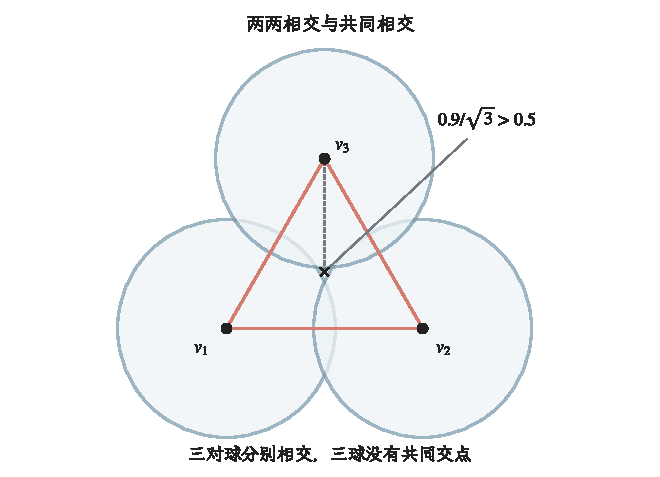
\includegraphics[width=\linewidth]{figures/01-mathematical-preliminaries/02-linear-algebra-and-geometry/matplotlib/teaching-linear-probability/geometry-cech-rips-intersection.pdf}
 \caption{固定同组三点比较共同交集与成对条件。正三角形边长$0.9$，
 $\varepsilon=1$，蓝色开球半径$0.5$；红色边满足两种构造的连边条件。
 三球无共同交点，Čech不含二维面，Rips含二维面。
 中心到各顶点的距离为$0.9/\sqrt3>0.5$。圆周只标开球边界，图为解析教学构造。}
 \label{fig:geometry-cech-rips-intersection}
\end{figure}

尺度变化后仍可给出明确包含关系。对任意$\eta>0$，有
\[
 \mathcal C_\varepsilon\subseteq\mathcal R_\varepsilon
 \subseteq\mathcal C_{2\varepsilon+\eta}.
\]
第一个包含关系由共同交点和三角不等式推出。
对第二个，任选一个顶点作候选共同交点，它到其余顶点的距离至多$\varepsilon$，
严格小于新球半径$\varepsilon+\eta/2$。
若全部球改用闭球，在相应定义下可取尺度常数$2$而不加$\eta$。
这些是足够的普适常数，不声称最紧；同一尺度的复形仍不能互换。

复形何时能代表球并集的拓扑，还依赖覆盖条件。良好覆盖（good cover）要求每个
非空有限交集都可连续收缩到一点；有限欧氏开球的交集为凸集，满足这项要求。
神经引理（nerve lemma）在该条件下说明Čech复形与球并集同伦等价，即二者存在相互映射，
来回复合可以连续变形到恒等映射。这里不要求两映射互为逆，所以比同胚弱：
闭区间可连续收缩到一个点，与单点空间同伦等价，却不可能与它存在双射。
这个结论不等于球并集已经恢复了未知潜在流形；
后者还需要采样覆盖和尺度条件。

为计算未被填充的环，需要把端点抵消与高阶填充分别记录。
选定顶点次序后，以$[v_0,\ldots,v_k]$表示有向单纯形，交换两顶点使符号反转。
有向$k$维单纯形的实系数线性组合称为$k$维链，
组成向量空间$C_k(\mathcal K;\mathbb R)$。边界算子读取每个面的有向边缘：
\begin{equation}
 \partial_k[v_0,\ldots,v_k]
 =\sum_{i=0}^k(-1)^i[v_0,\ldots,\widehat{v_i},\ldots,v_k],
 \qquad k\geq1,
 \label{eq:geometry-simplicial-boundary}
\end{equation}
尖帽表示删去该顶点，算子线性延伸到全部链。
本章采用非约化同调，约定$C_{-1}=\{0\}$、$\partial_0=0$。
例如$\partial_1[1,2]=[2]-[1]$，端点的正负表示方向。

\begin{lemma}[边界的边界为零]
\label{lem:geometry-boundary-squared-zero}
上述算子满足
\begin{equation}
 \partial_{k-1}\partial_k=0,\qquad k\geq1.
 \label{eq:geometry-boundary-squared-zero}
\end{equation}
\end{lemma}
\begin{proof}
$k=1$时由$\partial_0=0$成立。对$k\geq2$，固定$i<j$，
两次删除$v_i,v_j$后得到相同的$(k-2)$维面。
先删$i$再删原来的$j$，系数为$(-1)^i(-1)^{j-1}$；
先删$j$再删$i$，系数为$(-1)^j(-1)^i$，两者相反。
所有项都按这样的顶点对成对抵消，因此结论对基单纯形成立；
由线性性，对全部链成立。
\end{proof}

边界必定闭合，但闭合的圈未必由复形中的某个面填充。
这正好可以用上一章的核、像与商空间表达。
\begin{definition}[闭链、边界与同调空间]
\label{def:geometry-homology-space}
满足$\partial_kc=0$的链称为\term{闭链}（cycle），
能写成$c=\partial_{k+1}b$的链称为\term{边界}（boundary）。
由$\partial_k\partial_{k+1}=0$，有
$\operatorname{im}\partial_{k+1}\subseteq\ker\partial_k$。
实系数\term{同调空间}（homology space）及其维数定义为
\[
 H_k(\mathcal K;\mathbb R)=\ker\partial_k/\operatorname{im}\partial_{k+1},
 \qquad \beta_k=\dim H_k(\mathcal K;\mathbb R).
\]
$\beta_k$称为第$k$个\term{Betti数}（Betti number）。
\end{definition}
商空间沿用定义~\ref{def:linear-algebra-quotient-space}：
两个闭链相差一个边界时被视为同类。因而$H_k$保留的不是全部闭链，
而是无法用已有高阶填充消去的部分；$\beta_0$计算连通分支，
$\beta_1$计算实系数意义下独立的一维环。

取
$\mathcal K_{\mathrm{loop}}
=\{\{1\},\{2\},\{3\},\{1,2\},\{2,3\},\{1,3\}\}$。
链$c=[1,2]+[2,3]-[1,3]$的端点逐一抵消，故$\partial_1c=0$。
$\partial_1$的秩为$2$，一维闭链空间维数为$3-2=1$，
而没有二维面，故$\beta_1=1$、$\beta_0=3-2=1$。
加入$[1,2,3]$后，$c=\partial_2[1,2,3]$成为边界，$\beta_1$降为$0$；
$\partial_1$不变，所以$\beta_0$仍为$1$。
图~\ref{fig:geometry-cycle-filled-simplex}只改变面集合，顶点与边保持相同。
\begin{figure}[htbp]
 \centering
 % Two finite simplicial complexes with the same vertices and edges.
% Intended canvas: 112 mm by 36 mm. Exact combinatorial teaching construction.
\begin{tikzpicture}[x=1cm,y=1cm,font=\figurefont\small,text=FigureInk,
  line width=1.1pt,draw=FigureStroke]
 \path[use as bounding box] (0,0) rectangle (11.2,3.6);
 \begin{scope}[shift={(1.3,0.75)}]
  \coordinate (a) at (0,0); \coordinate (b) at (2.4,0);
  \coordinate (c) at (1.2,1.75);
  \draw (a)--(b)--(c)--cycle;
  \foreach \v in {a,b,c} \fill[FigureInk] (\v) circle (1.3pt);
  \node[below] at (a) {$1$}; \node[below] at (b) {$2$};
  \node[above] at (c) {$3$};
  \node at (1.2,2.5) {空心三角环};
  \node at (1.2,-0.55) {$\beta_1=1$};
 \end{scope}
 \begin{scope}[shift={(7.0,0.75)}]
  \coordinate (a) at (0,0); \coordinate (b) at (2.4,0);
  \coordinate (c) at (1.2,1.75);
  \fill[FigureYellowFill] (a)--(b)--(c)--cycle;
  \draw (a)--(b)--(c)--cycle;
  \foreach \v in {a,b,c} \fill[FigureInk] (\v) circle (1.3pt);
  \node[below] at (a) {$1$}; \node[below] at (b) {$2$};
  \node[above] at (c) {$3$};
  \node at (1.2,2.5) {填充三角面};
  \node at (1.2,-0.55) {$\beta_1=0$};
 \end{scope}
\end{tikzpicture}%

 \caption{一圈边是否已填充，取决于高阶面而非边图。左侧闭链
 $c=[1,2]+[2,3]-[1,3]$不是边界；右侧加入$[1,2,3]$后有
 $c=\partial_2[1,2,3]$。两者$\beta_0=1$，$\beta_1$分别为$1$与$0$。
 图为组合教学示例，不代表某个观测点云的真实拓扑。}
 \label{fig:geometry-cycle-filled-simplex}
\end{figure}

复形的规模还依赖邻域尺度。开带$\mathcal M_{\mathrm{strip}}$与开矩形同胚，
中心线$\mathcal C$与开区间同胚，都没有全局环。
闭合中心线得到圆，保留横向自由度并闭合则得到二维环带；
维数不同，但都保留绕中心的一维环。只有在采样和尺度适当时，样本复形才有理由
反映这些区别。尺度太小会把采样空隙误认作分支；太大则可能跨折连边，
并以高阶面填掉原来的环。

单一尺度可能把采样空隙当成孔洞，也可能把真实孔洞填平。持续同调（persistent homology）
因此跟踪尺度逐渐增大时，同调类何时出现、何时消失。存在于较宽尺度范围内的结构
提供了跨尺度信息，但仍不能仅凭持续时间就认定它对应任务中的真实结构。
若$N_k$是$k$维单纯形数，Euler示性数
$\chi=\sum_k(-1)^kN_k$是更粗的摘要：空心三角形为$3-3=0$，
填充三角形为$3-3+1=1$。由秩--零度关系
$N_k=\beta_k+\operatorname{rank}\partial_k+\operatorname{rank}\partial_{k+1}$，
交替求和后中间秩抵消，也得到$\chi=\sum_k(-1)^k\beta_k$。
不同Betti数组甚至不同拓扑都可能有同一个$\chi$，一个标量不足以代替分别分析。

用硬阈值连边时，两点距离只要稍微超过阈值，就会从相连突然变成不相连。为了记录
接近程度，可以改用软关系，以$\mu_{i,j}\in[0,1]$表示所选局部尺度下的连接强度；
这只是隶属度，不自动是事件概率。高阶强度例如可取全部边强度的最小值，
但必须声明采用哪种规则。一种常见的合并运算是
\begin{equation}
 a\mathbin{\sqcup}b=a+b-ab=1-(1-a)(1-b),\qquad a,b\in[0,1].
 \label{eq:geometry-fuzzy-union}
\end{equation}
结果仍在$[0,1]$内；交换性由对称式给出，结合性由
$1-(1-a)(1-b)(1-c)$给出，$0$为恒等元，任一输入为$1$时输出为$1$。
这些性质使它成为明确定义的软并集，却没有提供独立事件的随机试验或联合分布。
核权重、相似度、置信度与概率的校准要求不能仅凭数值范围混同。

UMAP等方法由局部距离构造带强度的关系，再优化低维坐标以匹配这些关系；
具体目标与优化过程留给
\BookChapterRef{chap:dimensionality-reduction}{第三卷“模型”的“降维”章}。
低维图像中的分离簇或孔洞还可能受邻居数、尺度、初始化与优化误差影响。
拓扑方法不能修复错误的局部输入：跨折捷径会被忠实组合，完全漏采的区域也无法凭空
恢复。采样覆盖、局部关系与尺度共同限制结论。

局部坐标之间的过渡只有在区域衔接时才能复合。若要统一记录这种“有起点和终点的
变换”，可以使用\term{范畴}（category）：
它包含对象、对象之间的箭头及各对象的恒等箭头，
仅在端点匹配时复合箭头，复合满足结合律与恒等律。
函子（functor）把对象和箭头映到另一范畴，同时保持恒等与复合。
例如坐标区域间可复合的过渡可按这种方式记录。
这只是组合表示的延伸语言，本章的距离与同调推导均不依赖它，
也不因引入这些名称获得额外的恢复保证。

\section{非线性空间的局部线性化}
\label{sec:geometry-manifold-local-linearization}

坐标图记录位置，却还没有说明从当前位置可以怎样动。以下固定光滑流形模型，
以局部参数化计算真实的一阶方向，再讨论只有样本时怎样估计这些方向。
解析模型与样本估计解决同一个局部问题，但它们的输入与保证不同。

\subsection{已知参数化下的局部线性化}
\label{sec:geometry-analytic-local-linearization}

从$\bm p=\varphi(\bm z)$出发，坐标变化$\bm v$经Jacobian
$\bm J_\varphi(\bm z)$映为环境空间中的瞬时速度。
\term{切空间}（tangent space）收集所有这样的可行速度；
它描述一阶方向，并不是可行集合本身的一小块。

\begin{definition}[嵌入流形的切空间]
\label{def:geometry-tangent-space}
设$\varphi:U\subseteq\mathbb R^d\to\mathcal M\subseteq\mathbb R^D$
是局部参数化，$\bm p=\varphi(\bm z)$。定义
\begin{equation}
 T_{\bm p}\mathcal M
 =\{\bm J_\varphi(\bm z)\bm v:\bm v\in\mathbb R^d\}.
 \label{eq:geometry-tangent-space-chart}
\end{equation}
\end{definition}
Jacobian列满秩保证这是$d$维向量空间，其原点是零速度。
画在$\bm p$旁边的仿射切平面则是$\bm p+T_{\bm p}\mathcal M$；
点的位置与速度向量的零点不能混为一谈。

\begin{lemma}[曲线速度与坐标刻画相容]
\label{lem:geometry-tangent-curves}
$T_{\bm p}\mathcal M$恰是全部光滑曲线
$\gamma:(-\epsilon,\epsilon)\to\mathcal M$、$\gamma(0)=\bm p$
的速度$\gamma'(0)$组成的集合，并且与局部坐标选择无关。
\end{lemma}
\begin{proof}
在足够小的参数区间内，曲线落入当前坐标图，写成
$\gamma(t)=\varphi(\bm z(t))$。链式法则给出
$\gamma'(0)=\bm J_\varphi(\bm z)\bm z'(0)$，故每个曲线速度都属于所定义的空间。
反过来，任意$\bm v\in\mathbb R^d$给出曲线
$t\mapsto\varphi(\bm z+t\bm v)$；因为$U$开，足够小的$t$仍在定义域内，
其初速度为$\bm J_\varphi(\bm z)\bm v$。

若另一参数化满足$\widetilde\varphi=\varphi\circ\psi$，
坐标过渡$\psi$的Jacobian可逆，且
$\bm J_{\widetilde\varphi}=\bm J_\varphi\bm J_\psi$。
右乘可逆矩阵不改变值域，两张图因而给出同一切空间。
\end{proof}

在点带中直接求导，可核对两个自由度：
\begin{align}
 \frac{\partial\Phi}{\partial s}
 &=\left(1+\frac uR\right)
   \begin{bmatrix}-\sin(s/R)\\\cos(s/R)\end{bmatrix},
 \label{eq:geometry-strip-s-tangent}\\
 \frac{\partial\Phi}{\partial u}
 &=\begin{bmatrix}\cos(s/R)\\\sin(s/R)\end{bmatrix}.
 \label{eq:geometry-strip-u-tangent}
\end{align}
因$|u|<w<R$，第一列不为零，两列正交且线性无关；
开带的切空间是整个$\mathbb R^2$。中心线则只允许$u=0$，
\[
 T_{\Phi(s,0)}\mathcal C
 =\operatorname{span}\{(-\sin(s/R),\cos(s/R))^\top\}.
\]
径向方向对开带可行，对中心线不可行。中心线的切线随位置转动，
没有一条固定线性子空间等于各处的切空间。

图~\ref{fig:geometry-strip-tangent-coordinates}上半部把切向速度画在点旁，
下半部比较同一坐标增量对应的实际弧长。方向数目决定局部维数，
坐标增量怎样换算为长度则留待度量处理。
\begin{figure}[htbp]
 \centering
 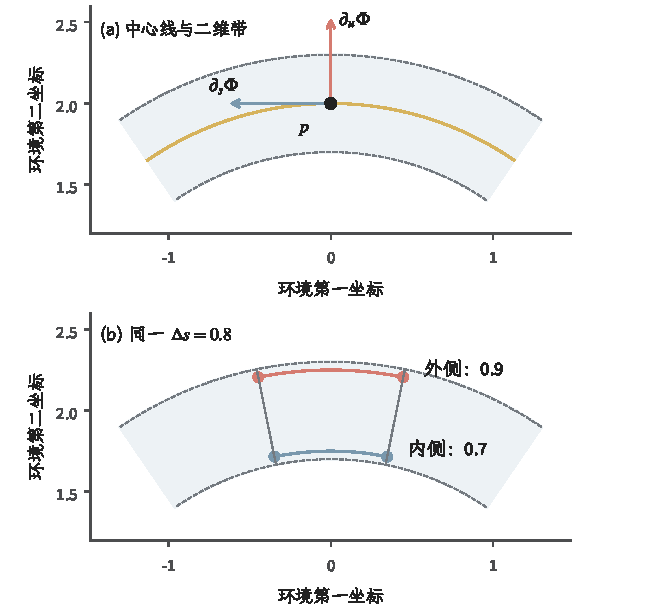
\includegraphics[width=\linewidth]{figures/01-mathematical-preliminaries/02-linear-algebra-and-geometry/matplotlib/concepts-linear-geometry/geometry-strip-tangent-coordinates.pdf}
 \caption{开带与中心线的局部方向不同。取$R=2$、$w=0.3$。
 上图的两个参数方向属于二维开带，仅以中心线为对象时，径向方向不属于其切空间；
 箭头平移到$\bm p$只是画法。下图取$u=-0.25,0.25$，同一$\Delta s=0.8$
 对应圆弧长度$0.7,0.9$。灰虚线为不纳入开带的边界，两图等比例绘制，均为解析教学示例。}
 \label{fig:geometry-strip-tangent-coordinates}
\end{figure}

切空间之所以适合近似，由Taylor展开说明。若参数化在当前邻域内二阶导数有界，则
\begin{equation}
 \varphi(\bm z+\bm h)-\varphi(\bm z)
 =\bm J_\varphi(\bm z)\bm h+O(\lVert\bm h\rVert_2^2).
 \label{eq:geometry-manifold-local-taylor}
\end{equation}
一阶项属于切空间，故环境位移投到法向正交补后只剩二阶余项。
这是局部结论，常数依赖所选邻域及二阶导数界；不能将它延伸到任意大步长。
法向偏离反映嵌入在环境中怎样弯曲，不等于后文要定义的内在曲率。
在二维开带中法向空间为零，弯曲坐标线本身就不构成法向误差。

若流形由约束$F(\bm x)=\bm0$给出，其中
$F:\mathbb R^D\to\mathbb R^{D-d}$在$\bm p$附近光滑且
$\bm J_F(\bm p)$行满秩，就能选出$D-d$列组成可逆方阵。
重排坐标后，定理~\ref{thm:analysis-implicit-function}把这$D-d$个变量
解为其余$d$个变量的光滑函数，后者便给出局部参数化。
对约束内曲线求导得$\bm J_F(\bm p)\gamma'(0)=\bm0$；
所以切空间包含于该矩阵的核。参数化给出$d$维切空间，
秩--零度关系又说明核为$d$维，故$T_{\bm p}\mathcal M=\ker\bm J_F(\bm p)$。
满秩条件不能省略：$F(x,y)=x^2+y^2$在原点导数为零，
核是整个平面，但零水平集只有一个点，真实可行速度只有零向量。

不仅位置可被映射，位置变化也需要随映射传递。
设$F:\mathcal M\to\mathcal N$，其坐标表达
$\psi^{-1}\circ F\circ\varphi$光滑，则称$F$光滑。
它在$\bm p$处的微分（differential）把输入速度转成输出速度：
\[
 \mathrm dF_{\bm p}(\bm v)
 =\left.\frac{\mathrm d}{\mathrm dt}F(\gamma(t))\right|_{t=0},
 \qquad\gamma(0)=\bm p,\quad\gamma'(0)=\bm v.
\]
若$\bm v=\bm J_\varphi(\bm z)\bm a$，令
$\bm w=\psi^{-1}(F(\bm p))$，则
\begin{equation}
 \mathrm dF_{\bm p}(\bm v)
 =\bm J_\psi(\bm w)
   \bm J_{\psi^{-1}\circ F\circ\varphi}(\bm z)\bm a.
 \label{eq:geometry-map-differential}
\end{equation}
右端只依赖初速度，不依赖实现速度的曲线，因此定义良好且线性。
坐标变换时两侧的Jacobian因链式法则相互抵消；
$\mathrm dF_{\bm p}:T_{\bm p}\mathcal M\to T_{F(\bm p)}\mathcal N$
是几何映射，矩阵只是其坐标记录。复合还满足
$\mathrm d(H\circ F)_{\bm p}=\mathrm dH_{F(\bm p)}\circ\mathrm dF_{\bm p}$。

对标量函数$f:\mathcal M\to\mathbb R$，微分读取速度引起的一阶数值变化。
\term{余切空间}（cotangent space）$T_{\bm p}^*\mathcal M$就是
$T_{\bm p}\mathcal M$的线性泛函空间，泛函的含义沿用
定义~\ref{def:functional-bounded-linear-functional}。
有限维向量空间上的全部线性读取组成其对偶空间（dual space）；
所以$\mathrm df_{\bm p}\in T_{\bm p}^*\mathcal M$，不是一个切向量。
写局部坐标为$(z^1,\ldots,z^d)$时，上标在这里是坐标编号而非迭代次数。
坐标切基为$\partial_i=\partial\varphi/\partial z^i$，
其对偶基$\mathrm dz^i$满足$\mathrm dz^i(\partial_j)=\delta_{i,j}$，
也就是$\mathrm dz^i(\sum_j a^j\partial_j)=a^i$：它读出速度的第$i$个坐标系数。于是
\[
 \mathrm df=\sum_i\partial_i(f\circ\varphi)\,\mathrm dz^i,\qquad
 \mathrm df\!\left(\sum_i a^i\partial_i\right)
 =\sum_i\partial_i(f\circ\varphi)a^i.
\]
例如圆上$f(\cos\theta,\sin\theta)=\cos\theta$，
角速度$a$对应的数值变化为$-a\sin\theta$。
要把这个线性读取规则表示成“最陡方向”，还须指定方向长度，
所以梯度将在度量建立后定义。

\subsection{观测样本下的局部线性化}
\label{sec:geometry-sampled-local-linearization}

只有$\bm x_i=\bm p_i+\bm\epsilon_i$时，参数化与潜在位置通常未知。
我们可以考察附近样本主要沿哪些方向变化，用这些方向近似真实切空间。局部PCA
（local principal component analysis）就是按这个思路，在小邻域中寻找主要的线性
变化方向。它估计一个已经选定的流形模型，并不定义流形本身。
必须先说明潜在对象是二维带还是一维中心线，才能确定希望估计什么。

给观测$\bm x_i$选择邻居索引集$N_i$和权重
$\alpha_{i,j}\geq0$、$\sum_{j\in N_i}\alpha_{i,j}=1$，计算
\begin{equation}
 \overline{\bm x}_i=\sum_{j\in N_i}\alpha_{i,j}\bm x_j,\qquad
 \bm C_i=\sum_{j\in N_i}\alpha_{i,j}
  (\bm x_j-\overline{\bm x}_i)(\bm x_j-\overline{\bm x}_i)^\top.
 \label{eq:geometry-local-weighted-covariance}
\end{equation}
若潜在维数$d$给定，取$\bm C_i$最大$d$个特征值对应的正交特征向量
$\widehat{\bm U}_i$，其列空间$\widehat T_i$为估计方向子空间。
若$d$未知，需另由谱和误差模型判断；不能把预先指定的特征向量数当成维数发现。
局部均值消去样本位置偏移，但不保证等于$\bm p_i$。

计算结果要与真实对象分开。$T_{\bm p_i}\mathcal M$是潜在位置处的真实方向空间，
$\widehat T_i$是从样本估计出的方向空间，二者都以零速度为原点。把估计方向空间
平移到$\overline{\bm x}_i$或$\bm x_i$处，才得到图中画出的仿射切平面近似。
若$d<D$，一般环境噪声使$\bm x_i\notin\mathcal M$，
此时$T_{\bm x_i}\mathcal M$甚至没有定义。
二维开带是当前例外：小噪声下观测仍在开带内，其切空间仍为$\mathbb R^2$，
但这不表示已经识别出生成它的潜在位置。

式~\eqref{eq:geometry-manifold-local-taylor}解释了误差来源。
在正则局部坐标中，邻域尺度为$h$时，切向位移通常为$O(h)$，
嵌入法向偏离为$O(h^2)$。若采样在各切方向上充分展开，
切向协方差特征值具有$h^2$量级；法向位移的平方贡献则可达到$h^4$量级。
这些尺度比较需要二阶导数有界和非退化局部采样，单靠光滑性并不保证谱间隙。

上一章的子空间扰动结论可用于把误差变成方向误差：
若理想局部协方差在第$d$与第$d+1$特征值间有间隙$\delta>0$，
而观测造成的算子范数扰动相对$\delta$足够小，则估计子空间的偏转受
$\lVert\bm E\rVert_2/\delta$控制。这里$\bm E$要包括有限样本波动、
噪声、邻域错选及非线性近似误差，不能只代入测量噪声方差。

缩小邻域会降低法向二阶偏差，却减少样本并压低真实信号的谱尺度；
固定噪声不会随之自动消失。邻域过大时，中心线不同位置的切线已经明显转动，
PCA会把这些不同方向合在一起，结果未必接近中心点的切线。对二维窄带，若样本的横向覆盖不足或宽度小于噪声尺度，
第二个方向可能难以稳定识别，但潜在对象并不因此变成一维。
固定近邻数也不能解决非均匀密度带来的变化：稀疏处覆盖范围大，稠密处范围小。
潜在对象、采样密度、嵌入弯曲、邻域尺度、谱间隙和噪声必须一起解释。

即使局部方向估计准确，也尚未得到全局坐标。圆的每个邻域只有一个切方向，
却不能以单张无断点实坐标图覆盖。局部PCA提供的是后续几何计算的局部输入，
不是全局展开或任务语义正确性的保证。

\section{流形上相同切空间下的度量、距离与运动}
\label{sec:geometry-metric-path-geodesic}

这里每次比较的两个向量，都属于同一个点处的切空间。
沿路径时，速度可以属于随位置变化的切空间；计算长度只需在每个位置读出一个标量速度，
再把这些标量累计起来，不需要先把不同位置的向量搬到一起。

\subsection{同一点处的切向量度量}
\label{sec:geometry-same-point-metric}

切空间说明方向可不可行，却没有规定一单位坐标变化有多长。
点带外侧与内侧相同的$\mathrm ds$对应不同弧长，因而内积必须按位置指定。
\term{Riemann度量}（Riemannian metric）为每个切空间提供这种长度与夹角规则。

\begin{definition}[Riemann度量]
\label{def:geometry-riemannian-metric}
光滑流形$\mathcal M$上的Riemann度量$g$为每个$\bm p$指定内积
$g_{\bm p}:T_{\bm p}\mathcal M\times T_{\bm p}\mathcal M\to\mathbb R$，
且在任一光滑坐标切基$\partial_i$中，矩阵
$\bm G(\bm z)=[g_{i,j}(\bm z)]$、$g_{i,j}=g(\partial_i,\partial_j)$
的条目光滑。每个$\bm G$都对称正定。
\end{definition}
对同点切向量$\bm v,\bm w$，长度为
$\lVert\bm v\rVert_g=\sqrt{g_{\bm p}(\bm v,\bm v)}$；
非零时夹角满足
$\cos\vartheta=g_{\bm p}(\bm v,\bm w)/
(\lVert\bm v\rVert_g\lVert\bm w\rVert_g)$。
若它们的坐标分量为$\bm a,\bm b$，内积是$\bm a^\top\bm G\bm b$。
$\bm G$既不是样本协方差，也不必是全空间共享的常矩阵。

嵌入流形可以限制环境欧氏内积，得到诱导度量：
\begin{equation}
 \bm G(\bm z)=\bm J_\varphi(\bm z)^\top\bm J_\varphi(\bm z).
 \label{eq:geometry-induced-metric}
\end{equation}
对非零$\bm a$，满列秩保证
$\bm a^\top\bm G\bm a=\lVert\bm J_\varphi\bm a\rVert_2^2>0$。
若Jacobian退化，只会得到半正定形式；这不符合当前坐标中的Riemann度量条件。
也可以另选光滑正定内积，但这样会改变几何，而不只是改写坐标。

若旧坐标$\bm z=\psi(\bm v)$，记可逆Jacobian为$\bm A=\bm J_\psi$，
同一几何向量的旧分量等于$\bm A$乘新分量，所以
\begin{equation}
 \widetilde{\bm G}(\bm v)=
 \bm A^\top\bm G(\psi(\bm v))\bm A.
 \label{eq:geometry-metric-coordinate-transform}
\end{equation}
因此$\bm a^\top\widetilde{\bm G}\bm b
=(\bm A\bm a)^\top\bm G(\bm A\bm b)$。
改变分量而不改变度量会改变所计算的长度；按此式一起变换则仍描述同一内积。

点带的两个参数方向已在式~\eqref{eq:geometry-strip-s-tangent}与
\eqref{eq:geometry-strip-u-tangent}中求出，故
\begin{equation}
 \bm G(s,u)=
 \begin{bmatrix}(1+u/R)^2&0\\0&1\end{bmatrix}.
 \label{eq:geometry-strip-metric}
\end{equation}
横向速度$\dot u$的长度系数为$1$，纵向速度$\dot s$的系数为$1+u/R$。
在$R=2$、$u=\pm0.25$时，同一$\Delta s=0.8$沿固定$u$的圆弧
分别产生$0.9$与$0.7$的长度，与图~\ref{fig:geometry-strip-tangent-coordinates}一致。
内积权重来自坐标尺度，并不由该位置采到了多少点决定。

\subsection{沿路径的速度与长度}
\label{sec:geometry-path-speed-length}

设分段光滑路径$\gamma:[a,b]\to\mathcal M$在一张图中写成
$\gamma(t)=\varphi(\bm z(t))$。链式法则保证
$\dot\gamma(t)\in T_{\gamma(t)}\mathcal M$，度量读出的平方速度为
\begin{equation}
 \lVert\dot\gamma(t)\rVert_g^2
 =\dot{\bm z}(t)^\top\bm G(\bm z(t))\dot{\bm z}(t).
 \label{eq:geometry-riemannian-speed}
\end{equation}
将标量速度按时间累计，定义路径长度
\begin{equation}
 L_g(\gamma)=\int_a^b
 \sqrt{\dot{\bm z}(t)^\top\bm G(\bm z(t))\dot{\bm z}(t)}\,\mathrm dt.
 \label{eq:geometry-riemannian-curve-length}
\end{equation}
整条路径不在同一张图时，将紧区间$[a,b]$分成有限段，使每段落入一张图，
再求长度之和。紧致的路径像和坐标开覆盖保证能作这种有限分段。

这种计算不依赖坐标。在$\bm z=\psi(\bm v)$下，
$\dot{\bm z}=\bm A\dot{\bm v}$，
式~\eqref{eq:geometry-metric-coordinate-transform}给出
$\dot{\bm v}^\top\widetilde{\bm G}\dot{\bm v}
=\dot{\bm z}^\top\bm G\dot{\bm z}$。
每段被积的标量相同，所以重叠区域选哪张图、怎样进一步细分都不改变长度。

长度也不依赖沿同一路线前进的快慢。对保持方向的光滑重参数化$t=\tau(r)$，
新速度为$\dot\gamma(\tau(r))\tau'(r)$，
其长度因子为$|\tau'(r)|$；当$\tau'>0$时，
积分换元$\mathrm dt=\tau'(r)\mathrm dr$给出相同总长。
反向的光滑单调参数化配合积分端点互换也不改变长度。
允许停顿的分段正则重参数化可分段处理；来回多走则改变路线的经过次数，
不属于仅仅换速度。

瞬时切向可行不等于环境直线可行。单位圆上
$\bm p=(1,0)^\top$、$\bm v=(0,1)^\top\in T_{\bm p}\mathbb S^1$，
但$\lVert\bm p+t\bm v\rVert_2=\sqrt{1+t^2}>1$对$t\neq0$成立。
速度只描述路径的一阶变化，保持有限步可行仍需在曲面上构造完整路径或更新映射。

\subsection{固定端点间的测地距离与近似}
\label{sec:geometry-endpoint-distance}

路径长度评价一条已经给出的路线。端点固定而路线可选时，要比较所有允许的路线；
完整空间已知和只有有限采样是这个问题的两种信息条件。

\subsubsection{连续空间下的测地距离}
\label{sec:geometry-continuous-geodesic-distance}

\begin{definition}[测地距离]
\label{def:geometry-geodesic-distance}
在Riemann流形$(\mathcal M,g)$的同一路径连通分支内，定义
\term{测地距离}（geodesic distance）为连接两点的全部分段光滑路径长度的下确界：
\begin{equation}
 d_g(\bm p,\bm q)=
 \inf_{\substack{\gamma(a)=\bm p\\\gamma(b)=\bm q}}L_g(\gamma).
 \label{eq:geometry-geodesic-distance}
\end{equation}
若无连接路径，约定值为$+\infty$；在可能不连通的整个空间上，它是扩展距离。
\end{definition}
这里的定义尚不要求存在最短路径，更不依赖测地线方程。
反向路径给出对称性，拼接两条近似最短路径给出三角不等式。
在一个足够小的坐标邻域内，按度量计算的向量长度，可以用其坐标向量的欧氏长度
乘以两个固定正常数从上下控制。这保证不同点之间的路程不能趋于零，因而每个
连通分支中确实得到度量。

对于欧氏诱导度量，由
$\bm q-\bm p=\int_a^b\dot\gamma(t)\,\mathrm dt$与三角不等式，
每条连接路径均满足$\lVert\bm q-\bm p\rVert_2\leq L_g(\gamma)$，
所以
\[
 \lVert\bm q-\bm p\rVert_2\leq d_g(\bm p,\bm q).
\]
若连接线段完全可行，就取等。反过来，只有下确界被允许路径达到时，
取等才迫使该最短路径沿线段行进，至多改变速度；
距离相等本身不保证线段可行。若换成任意非诱导度量，上述环境距离比较也不能照搬。

回到开中心线的两点$\bm p=\Phi(s,0)$、$\bm q=\Phi(t,0)$。
环境空间的弦长是
\begin{equation}
 \lVert\Phi(s,0)-\Phi(t,0)\rVert_2
 =2R\left|\sin\frac{s-t}{2R}\right|.
 \label{eq:geometry-strip-chord-distance}
\end{equation}
中心线以$s$为弧长参数，允许路径必须留在开弧内，因此
$d_{\mathcal C}(\bm p,\bm q)=|s-t|$。
二维带允许路径向内侧绕行，中心线弧只是候选，故
\[
 \lVert\bm p-\bm q\rVert_2
 \leq d_{\mathcal M_{\mathrm{strip}}}(\bm p,\bm q)
 \leq d_{\mathcal C}(\bm p,\bm q)=|s-t|.
\]
带宽、端点位置和允许域决定第二个不等式是否严格；
不能把这两种距离都称为不加区分的“沿带距离”。

另取完整单位圆作为独立例子。夹角$0\leq\theta\leq\pi$时，
允许选择短弧，内在距离为$\theta$，弦长为$2\sin(\theta/2)$。
在$\theta=\pi/2$时两者为$\pi/2$与$\sqrt2$；
小角度展开$2\sin(\theta/2)=\theta-\theta^3/24+O(\theta^5)$说明局部接近，
全局却不同。图~\ref{fig:geometry-circle-distances}在相同尺度上比较这两种量。
\begin{figure*}[htbp]
 \centering
 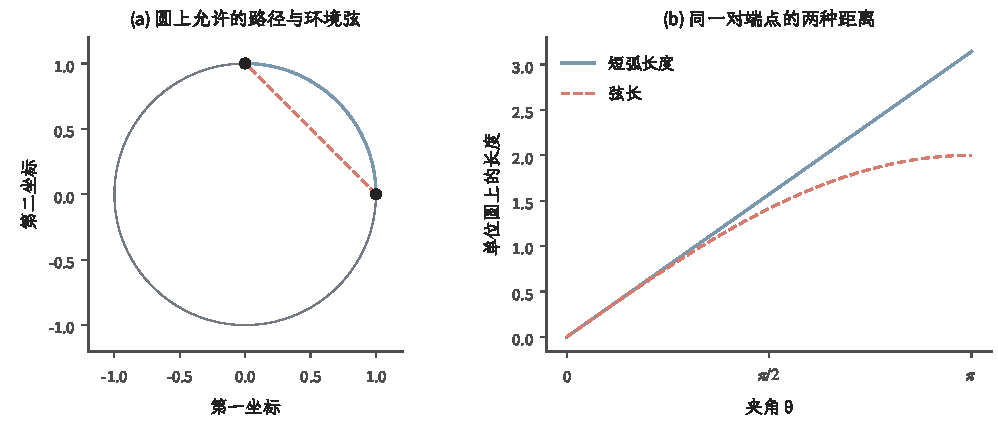
\includegraphics[width=\linewidth]{figures/01-mathematical-preliminaries/02-linear-algebra-and-geometry/matplotlib/analysis-geometry/geometry-circle-distances.pdf}
 \caption{完整单位圆的测地距离与环境弦长。左图夹角为$\pi/2$，
 蓝线为圆上的允许短弧，红虚线为穿过圆内的环境线段；
 右图比较$\theta\in[0,\pi]$时的两种长度。完整圆允许选择两段弧中的较短者，
 不能与开中心线或二维开带的允许路径混用。图为解析教学示例。}
 \label{fig:geometry-circle-distances}
\end{figure*}

为什么定义取下确界，而不直接取最小值？因为允许的路径未必包含一条最短路径。在穿孔平面
$\mathbb R^2\setminus\{\bm0\}$中，$(-1,0)^\top$与$(1,0)^\top$
之间可绕过任意小的圆孔，路径长度趋于$2$，却没有长度恰为$2$的允许路径。
哪些全局条件保证达到下确界，将在固定端点的最短路径问题中讨论。

\subsubsection{有限采样下的测地距离近似}
\label{sec:geometry-sampled-geodesic-distance}

只有观测点时，常把距离小于阈值$\varepsilon$的点相连，
或连接每个点的$k$个最近邻，再以$\lVert\bm x_i-\bm x_j\rVert_2$为边长。
一条边路径的长度是所经边长之和，最短边路径试图近似所选潜在流形上
$d_g(\bm p_i,\bm p_j)$。这里只借用顶点、边和路径的直观含义，
通用图算法留给第~\ref{part:discrete-mathematics-and-graph-theory}部分。

潜在对象必须先定。若观测不在潜在流形上，$d_g(\bm x_i,\bm x_j)$便未定义；
即使观测在二维开带内，也不能因此把它认作$\bm p_i$。
环境欧氏边长自然对应欧氏诱导度量的局部近似；
若目标采用另一个Riemann度量，就要据此修正边长，不能继续沿用欧氏弦长而声称目标未变。

邻域应足够小，使每条边只连接潜在流形上近似平直的一小段，避免把环境中靠得很近、
沿流形却相距很远的两段直接相连；
又要大到样本间的空隙能够连通。超过跨折环境间隔会引入捷径，低估沿潜在空间的距离；
小于采样空隙则会把一个真实分支拆开，返回无穷距离。
即使没有捷径，局部弦长误差与离散路径绕行误差也会共同作用，
不能无条件断言估计总在真实距离的同一侧。

固定$k$并不固定几何尺度。稀疏处第$k$个邻居可能很远，稠密处则很近，
有向近邻关系还可能不对称，需要声明如何对称化。
一致近似通常要求潜在流形光滑、采样在所研究区域逐渐稠密、
噪声相对邻域尺度受控，并让邻域半径随样本量缩小而仍足以覆盖采样空隙。
非紧开带若只在一部分采样，这些要求也只支持相应覆盖区域的结论。
具体收敛速度须结合采样分布与尺度选择证明，
最短边路径正确更不自动意味着后续全局坐标恢复正确。

\subsection{度量诱导的体积与积分}
\label{sec:geometry-riemannian-volume}

沿路径积分只覆盖一条路线。若要在整个曲面上累计函数值或变化量，就需要知道
每个小区域占多大面积；更高维时，相应的量是体积。
坐标切基围成的微小平行体，其平方体积是Gram行列式$\det\bm G$，
因此几何体积元为
\begin{equation}
 \mathrm dV_g=\sqrt{\det\bm G(\bm z)}\,\mathrm d\bm z.
 \label{eq:geometry-riemannian-volume}
\end{equation}
这是由度量产生的测度密度，不要求先为流形选定全局朝向。
一维时给出长度，二维时给出面积。

坐标变换$\bm z=\psi(\bm v)$下，
$\det\widetilde{\bm G}=(\det\bm A)^2\det\bm G$，所以
\[
 \sqrt{\det\widetilde{\bm G}}\,\mathrm d\bm v
 =\sqrt{\det\bm G(\psi(\bm v))}\,|\det\bm A|\,\mathrm d\bm v.
\]
它正是多元积分换元中的Jacobian因子，故对可积函数所得积分不依赖坐标。
跨图时必须避免把重叠区域重复计数，可分割成可测片段分别积分；
光滑计算也可使用从属于图册、和为$1$的局部权重来拼接。

点带中$\sqrt{\det\bm G}=1+u/R>0$，
小盒$\mathrm ds\,\mathrm du$在外侧对应较大面积。
中心线限制为$u=0$后的一维体积元是$\mathrm ds$，不是把二维面积直接代入。
若样本相对几何体积有密度$q$，其分布测度是$q\,\mathrm dV_g$；
简单样本平均近似该加权积分，并非自动近似$\int f\,\mathrm dV_g$。
几何体积与采样权重的差别将在离散平滑目标中再次出现。

当前开带无流形边界，但不是紧集。需要边界积分时，将另取有分片光滑边界的
截断闭域，并声明函数在边界的行为；不能只因图上画有虚线就把它当作同一个积分问题。

\section{流形上不同切空间的比较与曲率}
\label{sec:geometry-cross-point-comparison-curvature}

沿路径计算长度时，每个位置只输出一个标量。若要问速度有没有转弯，
或相邻两点的方向是否一致，就必须比较不同切空间中的向量。
即使流形嵌在同一个欧氏空间内，直接相减也可能产生法向分量：
圆上恒速运动的速度导数指向圆心，却没有沿圆加速。
需要把环境变化与流形内的方向变化分开。下面建立联络、测地运动和曲率，
所用的Riemann几何基础可参见Lee的教材\scite{math-lee2018riemannian}

\subsection{不同切空间的比较规则}
\label{sec:geometry-connection-comparison}

在每个位置指定一个可行方向，得到向量场。跨点比较规则应使其导数仍为切向量，
还应遵守加法和乘积求导；联络就是满足这些要求的微分规则。
它不是把所有切空间强行认成同一个空间，而是在局部说明怎样比较变化。

\begin{definition}[向量场与联络]
\label{def:geometry-connection}
光滑\term{向量场}（vector field）$\bm V$在每个$\bm p\in\mathcal M$选取
$\bm V(\bm p)\in T_{\bm p}\mathcal M$，其坐标分量光滑。
\term{联络}（connection）为两个光滑向量场$\bm U,\bm V$指定向量场
$\nabla_{\bm U}\bm V$，称为$\bm V$沿$\bm U$的
\term{协变导数}（covariant derivative），并满足
\[
 \begin{aligned}
 \nabla_{f\bm U+h\bm W}\bm V
   &=f\nabla_{\bm U}\bm V+h\nabla_{\bm W}\bm V,\\
 \nabla_{\bm U}(a\bm V+b\bm W)
   &=a\nabla_{\bm U}\bm V+b\nabla_{\bm U}\bm W,\\
 \nabla_{\bm U}(f\bm V)
   &=\bm U(f)\bm V+f\nabla_{\bm U}\bm V.
 \end{aligned}
\]
其中$f,h$为光滑函数，$a,b\in\mathbb R$，
$\bm U(f)=\mathrm df(\bm U)$为方向导数。
\end{definition}
第一条允许求导方向的系数是光滑函数，第二条只允许被求导向量场的系数是常数，
第三条说明为什么不能把第二条的常数任意换成光滑函数：
系数本身的变化必须保留。欧氏空间的普通方向导数满足这三项规则；
一般流形上，单独求坐标分量的导数不够，因为坐标切基本身也在变。

度量已经规定长度，新的导数应当与这一判断相容。
此外，非坐标方向场先后作用的顺序本来就可能不同，不能把这种差异误认为额外的几何扭转。
定义交换子$[\bm U,\bm V]$为对任意光滑$f$满足
\[
 [\bm U,\bm V](f)=\bm U(\bm V(f))-\bm V(\bm U(f))
\]
的向量场；在坐标基下，其第$k$个分量为
$\sum_i(U^i\partial_iV^k-V^i\partial_iU^k)$。
坐标方向$\partial_i,\partial_j$的交换子为零，一般方向场则未必。

\begin{example}[平面上不可交换的方向场]
\label{ex:geometry-plane-field-commutator}
在欧氏平面取$\bm U=\partial_x$、$\bm V=x\partial_y$。
$\bm U$始终沿$x$轴，$\bm V$沿$y$轴但其大小随$x$改变。
对任意光滑函数$f$，
\[
 \bm U(\bm V(f))=\partial_yf+x\partial_x\partial_yf,\qquad
 \bm V(\bm U(f))=x\partial_y\partial_xf,
\]
故$[\bm U,\bm V]=\partial_y$。先沿$x$方向移动，会改变随后沿$\bm V$移动的速度；
两个方向场的顺序差异在平面上就会出现。
欧氏空间的普通方向导数还给出
\[
 \nabla_{\bm U}\bm V=\partial_y,\qquad
 \nabla_{\bm V}\bm U=\bm0.
\]
二者之差恰是交换子。这个平坦例子说明，方向场本身随位置变化所产生的差异，
需要与几何结构额外产生的差异分开。
\end{example}

\begin{definition}[Levi--Civita联络]
\label{def:geometry-levi-civita-connection}
给定Riemann度量$g$，同时满足下列度量相容与无挠条件的联络，
称为它的\term{Levi--Civita联络}（Levi--Civita connection）：
\begin{align*}
 \bm U\bigl(g(\bm V,\bm W)\bigr)
 &=g(\nabla_{\bm U}\bm V,\bm W)+g(\bm V,\nabla_{\bm U}\bm W),\\
 \nabla_{\bm U}\bm V-\nabla_{\bm V}\bm U&=[\bm U,\bm V].
\end{align*}
\end{definition}
度量相容使内积的求导仍满足乘积法则；无挠规定联络在交换两个方向场时，
不产生交换子之外的差异。无挠\emph{不}声称
$\nabla_{\bm U}\nabla_{\bm V}\bm W
=\nabla_{\bm V}\nabla_{\bm U}\bm W$，后者涉及本节末尾的曲率。

每个光滑Riemann度量唯一确定这样的联络。其唯一性可以从两项条件直接看出：
轮换$\bm U,\bm V,\bm W$的度量相容等式，并用无挠条件消去交换项，得到
\begin{align}
 2g(\nabla_{\bm U}\bm V,\bm W)
 &=\bm U g(\bm V,\bm W)+\bm V g(\bm W,\bm U)
   -\bm W g(\bm U,\bm V)\notag\\
 &\quad+g([\bm U,\bm V],\bm W)-g([\bm V,\bm W],\bm U)
   +g([\bm W,\bm U],\bm V).
 \label{eq:geometry-koszul-formula}
\end{align}
右端只含已知度量、向量场和普通方向导数；正定性使其唯一确定
$\nabla_{\bm U}\bm V$。反过来，用此式定义该向量场，代入可检查联络的三条规则、
度量相容和无挠条件，因而也给出存在性。这个公式的用途是确定比较规则，
实际计算通常使用坐标系数或环境投影。

对继承欧氏度量的嵌入流形，设$\bm P_{\bm p}$为环境空间到
$T_{\bm p}\mathcal M$的正交投影，则
\begin{equation}
 \nabla_{\bm U}\bm V(\bm p)
 =\bm P_{\bm p}\,\mathrm d\bm V_{\bm p}(\bm U(\bm p)).
 \label{eq:geometry-projected-connection}
\end{equation}
这里把$\bm V$视为取值于环境$\mathbb R^D$的映射，先求环境导数再投影。
投影保持对切向量的内积，所以欧氏内积的乘积法则给出度量相容；
环境方向导数之差是已经切向的交换子，投影后仍不变，故也无挠。
由唯一性，这正是诱导度量的Levi--Civita联络。
若度量不是环境诱导度量，不能继续沿用这个欧氏正交投影公式。

\subsection{给定路径下的平行移动}
\label{sec:geometry-parallel-transport}

现在固定路径$\gamma(t)$和起点切向量，希望沿路保持方向。
“保持”不是要求环境坐标分量不变，而是要求联络测得的变化为零。
在坐标基中写
$\nabla_{\partial_i}\partial_j=\sum_k\Gamma^k_{i,j}\partial_k$，
则沿$\gamma(t)=\varphi(\bm z(t))$的向量
$\bm V(t)=\sum_jV^j(t)\partial_j$满足
\begin{equation}
 \frac{D\bm V}{\mathrm dt}
 =\sum_k\left(\dot V^k+
     \sum_{i,j}\Gamma^k_{i,j}(\bm z(t))\dot z^iV^j\right)\partial_k.
 \label{eq:geometry-covariant-derivative-along-path}
\end{equation}
第一项是分量变化，第二项修正坐标切基的变化；合起来才是坐标无关的协变导数。
对于欧氏诱导度量，式~\eqref{eq:geometry-projected-connection}沿路径写成
\[
 \frac{D\bm V}{\mathrm dt}
 =\bm P_{\gamma(t)}\frac{\mathrm d\bm V}{\mathrm dt},
\]
保留环境导数的切向部分。

\begin{definition}[平行移动]
\label{def:geometry-parallel-transport}
给定分段光滑路径$\gamma:[a,b]\to\mathcal M$和
$\bm v\in T_{\gamma(a)}\mathcal M$，沿路解
\[
 \frac{D\bm V}{\mathrm dt}=\bm0,\qquad \bm V(a)=\bm v.
\]
终值定义线性映射
$P_\gamma:T_{\gamma(a)}\mathcal M\to T_{\gamma(b)}\mathcal M$，
称为沿$\gamma$的\term{平行移动}（parallel transport）。
\end{definition}
坐标式是具有连续系数的线性常微分方程，初值唯一决定解；
沿有限段路径逐图求解并拼接即可，不要求流形完备。
反向路径给出逆映射，拼接路径对应映射复合。
对于Levi--Civita联络，
\[
 \frac{\mathrm d}{\mathrm dt}g(\bm V,\bm W)
 =g(D\bm V/\mathrm dt,\bm W)+g(\bm V,D\bm W/\mathrm dt)=0
\]
用于任意两个平行向量场。因此$P_\gamma$保持长度和夹角。
这个结论依赖度量相容，不能对任意联络直接宣称保距。

欧氏空间的直角坐标中$\Gamma^k_{i,j}=0$，平行移动保持向量的分量不变，
且与路径无关。球面则不同：向量必须始终切向，环境分量通常会改变，
不同路径的终值也可能不同。

\begin{example}[球面三段路径上的方向搬运]
\label{ex:geometry-sphere-parallel-transport}
在诱导度量的单位球面$\mathbb S^2$上，取
$N=(0,0,1)^\top$、$A=(1,0,0)^\top$、$B=(0,1,0)^\top$。
记三个坐标轴的单位向量为$\bm e_x,\bm e_y,\bm e_z$。
沿三条四分之一大圆弧$N\to A\to B\to N$搬运初始向量
$\bm V(N)=\bm e_x$。各段用$t\in[0,\pi/2]$参数化：
\[
 \begin{array}{c|c|c}
  \text{路径}&\gamma(t)&\bm V(t)\\ \hline
  N\to A&(\sin t,0,\cos t)^\top&(\cos t,0,-\sin t)^\top\\
  A\to B&(\cos t,\sin t,0)^\top&(0,0,-1)^\top\\
  B\to N&(0,\cos t,\sin t)^\top&(0,\sin t,-\cos t)^\top
 \end{array}
\]
每段都有$\gamma^\top\bm V=0$与$\lVert\bm V\rVert_2=1$。
第一段$\dot{\bm V}=-\gamma$，第二段$\dot{\bm V}=\bm0$，
第三段$\dot{\bm V}=\gamma$，环境导数全部是法向或零，投影后的协变导数为零。
两处接点的向量同为$-\bm e_z$，故三段连续拼接。
返回$N$时向量成为$\bm e_y$，与初始$\bm e_x$相差$\pi/2$。
若始终留在$N$，搬运则不改变向量，说明仅给起终点不能决定平行移动。
\end{example}

图~\ref{fig:geometry-sphere-parallel-transport}画出这些向量的沿路变化。
在$B\to N$段，向量与前进速度相反；保持方向不意味着向量必须指向前进方向。
\begin{figure}[htbp]
 \centering
 % Orthographic projection: x=(y-x)/sqrt(2), y=(2z-x-y)/sqrt(6).
% All tangent arrows have the same length before projection.
\begin{tikzpicture}[figure picture,x=1mm,y=1mm,
  transport/.style={draw=FigureRed,line width=.95pt,
    -{Stealth[length=1.8mm,width=1.2mm]}},
  route/.style={draw=FigureBlue,line width=1.1pt,
    -{Stealth[length=1.8mm,width=1.2mm]}},
  every node/.append style={fill=none,inner sep=1.2pt}]
 \path[use as bounding box] (0,10) rectangle (112,77);
 \begin{scope}[shift={(56,40)}]
  \draw[FigureGrid] (0,0) circle[radius=28];
  \draw[FigureGrid,dashed,samples=81,domain=135:315]
   plot ({28/sqrt(2)*(sin(\x)-cos(\x))},
         {-28/sqrt(6)*(cos(\x)+sin(\x))});
  \draw[FigureGrid,samples=81,domain=-45:135]
   plot ({28/sqrt(2)*(sin(\x)-cos(\x))},
         {-28/sqrt(6)*(cos(\x)+sin(\x))});
  \draw[route,samples=61,domain=0:90]
   plot ({-28/sqrt(2)*sin(\x)},
         {28/sqrt(6)*(2*cos(\x)-sin(\x))});
  \draw[route,samples=61,domain=0:90]
   plot ({28/sqrt(2)*(sin(\x)-cos(\x))},
         {-28/sqrt(6)*(cos(\x)+sin(\x))});
  \draw[route,samples=61,domain=0:90]
   plot ({28/sqrt(2)*cos(\x)},
         {28/sqrt(6)*(2*sin(\x)-cos(\x))});
  \foreach \t in {30,60} {
   \draw[transport]
    ({-28/sqrt(2)*sin(\t)},{28/sqrt(6)*(2*cos(\t)-sin(\t))})
    -- ++({-11/sqrt(2)*cos(\t)},
          {11/sqrt(6)*(-2*sin(\t)-cos(\t))});
   \draw[transport]
    ({28/sqrt(2)*(sin(\t)-cos(\t))},
     {-28/sqrt(6)*(cos(\t)+sin(\t))})
    -- ++(0,{-22/sqrt(6)});
   \draw[transport]
    ({28/sqrt(2)*cos(\t)},{28/sqrt(6)*(2*sin(\t)-cos(\t))})
    -- ++({11/sqrt(2)*sin(\t)},
          {11/sqrt(6)*(-2*cos(\t)-sin(\t))});
  }
  \coordinate (N) at (0,{56/sqrt(6)});
  \coordinate (A) at ({-28/sqrt(2)},{-28/sqrt(6)});
  \coordinate (B) at ({28/sqrt(2)},{-28/sqrt(6)});
  \draw[draw=FigureYellow,line width=1.2pt,
    -{Stealth[length=2mm,width=1.4mm]}]
    (N)--++({-11/sqrt(2)},{-11/sqrt(6)}) coordinate (Initial);
  \draw[transport] (N)--++({11/sqrt(2)},{-11/sqrt(6)})
    coordinate (Final);
  \foreach \p in {N,A,B} {\fill[FigureInk] (\p) circle[radius=.6];}
  \node[above] at (N) {$N$};
  \node[below left] at (A) {$A$};
  \node[below right] at (B) {$B$};
 \end{scope}
 \draw[FigureMuted,line width=.4pt] (Initial)--(36,70)--(26,70);
 \node[above] at (26,70) {初始 $\bm e_x$};
 \draw[FigureMuted,line width=.4pt] (Final)--(76,70)--(87,70);
 \node[above] at (87,70) {终值 $\bm e_y$};
\end{tikzpicture}

 \caption{单位球面上沿$N\to A\to B\to N$的平行移动。
 蓝色为给定的三条大圆弧，红箭头为例~\ref{ex:geometry-sphere-parallel-transport}
 中逐段计算的切向量。沿路协变导数为零，返回$N$后的方向却由黄色初始箭头
 $\bm e_x$变为红色终值箭头$\bm e_y$。
 箭头在三维中等长，投影到纸面后的长度可以不同。图为解析教学示例。}
 \label{fig:geometry-sphere-parallel-transport}
\end{figure}

这里的变换由路径和联络决定，不是任意选一个旋转来对齐环境向量。
前文群作用规定的是输入在指定变换下的响应；平行移动规定的是沿几何路径的方向比较，
即使二者有时都用矩阵表示，也不能据此互换。

\subsection{不同条件下的测地运动与最短路径}
\label{sec:geometry-geodesic-motion-minimization}

平行移动把路径当作输入、向量场当作未知量。若要求路径自己的速度平行移动，
路径也变成未知量。给定初速度时，这是运动方程的初值问题；
只给两个端点时，还要决定该沿哪条路径前进，最短性是额外的比较要求。

\subsubsection{初速度条件下的测地运动}
\label{sec:geometry-geodesic-initial-value}

\begin{definition}[测地线]
\label{def:geometry-geodesic}
相对于Riemann流形的Levi--Civita联络，采用仿射参数的曲线$\gamma$若满足
\[
 \frac{D\dot\gamma}{\mathrm dt}=\bm0,
\]
称为\term{测地线}（geodesic）。
\end{definition}
它没有切向加速度，速度沿自身路径作平行移动。
度量相容进一步给出
$\frac{\mathrm d}{\mathrm dt}\lVert\dot\gamma\rVert_g^2
=2g(D\dot\gamma/\mathrm dt,\dot\gamma)=0$，因此速度大小恒定。
环境加速度仍可非零，例如球面大圆需要法向加速度才能留在球面。

“仿射参数”说明换元$t=ar+b$、$a\neq0$保留这个方程。
一般换元则产生
\[
 \frac{D}{\mathrm dr}\frac{\mathrm d\gamma}{\mathrm dr}
 =(\tau'(r))^2\frac{D\dot\gamma}{\mathrm dt}
   +\tau''(r)\dot\gamma.
\]
非匀速参数化可以描出相同几何轨迹，却不再满足零协变加速度。
因此不能把路径长度的任意重参数化不变性照搬到这个运动方程。

要在坐标中求解，先用式~\eqref{eq:geometry-koszul-formula}取
$\bm U=\partial_i,\bm V=\partial_j,\bm W=\partial_\ell$。
坐标方向交换子为零，于是
\[
 2\sum_k g_{k,\ell}\Gamma^k_{i,j}
 =\partial_i g_{j,\ell}+\partial_j g_{i,\ell}-\partial_\ell g_{i,j}.
\]
乘逆度量便得到Christoffel符号
\begin{equation}
 \Gamma^k_{i,j}
 =\frac12\sum_{\ell=1}^d g^{k,\ell}
  \left(\frac{\partial g_{\ell,j}}{\partial z^i}
       +\frac{\partial g_{i,\ell}}{\partial z^j}
       -\frac{\partial g_{i,j}}{\partial z^\ell}\right),
 \qquad [g^{i,j}]=\bm G^{-1}.
 \label{eq:geometry-christoffel-symbols}
\end{equation}
将$\bm V=\dot\gamma=\sum_j\dot z^j\partial_j$代入
式~\eqref{eq:geometry-covariant-derivative-along-path}，测地条件成为
\begin{equation}
 \ddot z^k+\sum_{i,j=1}^d
 \Gamma^k_{i,j}(\bm z)\dot z^i\dot z^j=0.
 \label{eq:geometry-geodesic-equation}
\end{equation}
要判断这组系数是否表示点处的几何对象，需要区分几何张量与一张普通分量表。
这里的几何张量（geometric tensor）是点处、与坐标无关的多线性对象；
换基只对它的各个输入和输出作线性变换。因此，零分量表换基后仍为零。
Christoffel符号不满足这一规律。以正半轴的欧氏度量为例，
在坐标$x>0$中有$g_{x,x}=1$、$\Gamma^x_{x,x}=0$；
改用$x=e^u$后，$g_{u,u}=e^{2u}$，式~\eqref{eq:geometry-christoffel-symbols}给出
\[
 \Gamma^u_{u,u}=\frac12 e^{-2u}\frac{\mathrm d}{\mathrm du}e^{2u}=1.
\]
所以Christoffel符号是联络的坐标系数，不是张量。
基向量的变化与这些系数共同组成协变加速度，后者及所得曲线仍是几何对象。

有了这组坐标方程，就能由起点和初速度计算运动。光滑系数使这个二阶方程在给定
$\gamma(0)=\bm p$、$\dot\gamma(0)=\bm v$后具有局部唯一解，
并光滑依赖初值。这里“局部”同时限制时间和坐标覆盖范围；
可以换图延拓，但若路径有限时间离开流形，延拓就会失败。
开单位球内的欧氏直线从原点出发，以速度$2\bm e_1$前进，
在$t=1/2$时便到达不属于该流形的边界，不能默认解存在至$t=1$。

\begin{definition}[指数映射]
\label{def:geometry-exponential-map}
对给定$\bm p$，若初速度$\bm v$的测地线$\gamma_{\bm v}$存在至$t=1$，
定义
\[
 \operatorname{Exp}_{\bm p}(\bm v)=\gamma_{\bm v}(1).
\]
它称为$\bm p$处的\term{指数映射}（exponential map），
其定义域至少包含$T_{\bm p}\mathcal M$中零向量的一个邻域。
\end{definition}
初速度缩放对应时间缩放：
$\operatorname{Exp}_{\bm p}(t\bm v)=\gamma_{\bm v}(t)$，只在两边均有定义时使用。
因而$\operatorname{Exp}_{\bm p}(\bm0)=\bm p$且
$\mathrm d(\operatorname{Exp}_{\bm p})_{\bm0}=\operatorname{id}_{T_{\bm p}\mathcal M}$。
逆函数定理保证在足够小邻域中它是微分同胚；
这为用切向量表示附近点提供了一种局部方式，不保证全局一一对应。

单位球面上，$\bm v\perp\bm p$、$r=\lVert\bm v\rVert_2$时，
\begin{equation}
 \operatorname{Exp}_{\bm p}(\bm v)
 =\cos r\,\bm p+\frac{\sin r}{r}\bm v,
 \label{eq:geometry-sphere-exponential}
\end{equation}
$r=0$时按连续延拓取$\bm p$。
对应曲线$\gamma(t)=\cos(tr)\bm p+\sin(tr)\bm v/r$
满足$\lVert\gamma(t)\rVert_2=1$、初速度为$\bm v$，
且$\ddot\gamma=-r^2\gamma$为纯法向，所以确实解测地线方程。
所有方向上长度为$\pi$的初速度都到达对跖点$-\bm p$；
即使映射处处有定义，也未必全局单射。

\subsubsection{固定端点条件下的最短路径}
\label{sec:geometry-endpoint-minimizing-path}

现在给定$\bm p,\bm q$，要找一条长度真正等于
式~\eqref{eq:geometry-geodesic-distance}中下确界的路径。要说明最短路径为什么满足
测地线方程，可以先把长度问题转成更便于求导的能量问题。固定时间区间$[a,b]$，定义
\[
 E(\gamma)=\frac12\int_a^b\lVert\dot\gamma\rVert_g^2\,\mathrm dt.
\]
由Cauchy--Schwarz不等式，
$L_g(\gamma)^2\leq2(b-a)E(\gamma)$，等号恰对应几乎处处恒定的速度大小。
因此对可作匀速参数化的非退化路径，最小化长度可联系到固定时间的能量最小化；
能量本身却不具有长度那样的任意重参数化不变性。

在局部坐标中，Lagrange函数为
$\mathscr L(\bm z,\dot{\bm z})=\frac12\sum_{i,j}g_{i,j}(\bm z)\dot z^i\dot z^j$。
取光滑扰动$\bm h$，满足$\bm h(a)=\bm h(b)=\bm0$，并令
$\bm z_\varepsilon(t)=\bm z(t)+\varepsilon\bm h(t)$。
取足够小的$\varepsilon$使路径仍在坐标域内。
若$\varphi$为当前坐标的参数化，一阶变分就是把整条路径沿这个方向改变后，
能量关于扰动幅度的导数：
\[
 \delta E[\bm h]
 =\left.\frac{\mathrm d}{\mathrm d\varepsilon}
 E(\varphi\circ\bm z_\varepsilon)\right|_{\varepsilon=0}.
\]
对积分求导并分部积分，得到
\[
 \delta E[\bm h]
 =\int_a^b\sum_k\left(
 \frac{\partial\mathscr L}{\partial z^k}
 -\frac{\mathrm d}{\mathrm dt}
     \frac{\partial\mathscr L}{\partial\dot z^k}\right)h^k\,\mathrm dt.
\]
边界项因固定端点消失。驻定要求任意这样的$\bm h$都使变分为零，
因此括号中每个系数都必须为零：若某个连续系数在一点非零，
就在它保持同号的小邻域内取一个同号、光滑且在邻域外为零的扰动，
相应积分便不为零，产生矛盾。计算括号中的两个偏导得
\[
 \begin{aligned}
 \frac{\partial\mathscr L}{\partial z^k}
   &=\frac12\sum_{i,j}\partial_k g_{i,j}\dot z^i\dot z^j,\\
 \frac{\mathrm d}{\mathrm dt}
    \frac{\partial\mathscr L}{\partial\dot z^k}
   &=\sum_j g_{k,j}\ddot z^j+
     \sum_{i,j}\partial_i g_{k,j}\dot z^i\dot z^j.
 \end{aligned}
\]
对第二行的速度乘积对称化后，Euler--Lagrange方程为
\[
 \sum_jg_{k,j}\ddot z^j+
 \frac12\sum_{i,j}
  (\partial_i g_{k,j}+\partial_j g_{k,i}-\partial_k g_{i,j})
  \dot z^i\dot z^j=0.
\]
乘$\bm G^{-1}$即得式~\eqref{eq:geometry-geodesic-equation}。
跨图路径可对各段内支撑的扰动分别推导，得到相同几何方程。
这说明光滑匀速最短路必为测地线，不说明每个能量驻点都是最短路。

指数映射给出描述这些局部路径的区域。取零切向量附近的小开集$V$，
要求$\bm v\in V$时$t\bm v\in V$对$0\leq t\leq1$成立，
且$\operatorname{Exp}_{\bm p}$在$V$上为微分同胚。
它的像称为$\bm p$的正规邻域（normal neighborhood），
其中每个点都用一个初速度表示，径向路径对应$t\bm v$。
标准局部最短性结论保证可以把这个区域取到足够小，
使径向测地线段在邻域内达到端点间的最短长度。
还可进一步选择凸正规邻域（convex normal neighborhood），
让其中任意两点由唯一的邻域内最短测地线连接，整条线段留在该邻域中。
这里“凸”指测地线连接的性质，不是要求环境中的欧氏直线段留在区域内。
这项结论利用指数映射和径向、横向变化的正交性，不是只凭微分方程存在唯一性得到的。
离开这种局部范围后，其他路线可能更短。
若一段测地线达到$d_g$，称为\term{长度最短测地线}（length-minimizing geodesic）。

完整单位圆上，从$(1,0)^\top$到$(0,-1)^\top$的逆时针弧长为$3\pi/2$，
顺时针弧长为$\pi/2$。两条匀速圆弧都满足零协变加速度，
只有后者达到距离。相同的初值局部运动规则不承担全局路线比较。
割点研究从某点出发的测地线何时失去最短性，
共轭点涉及相邻测地线的聚焦与变分退化；这些进一步判据不在本章展开，
不能据术语本身判定一条路径最短。

\begin{theorem}[Hopf--Rinow定理的最短路存在性结论]
\label{thm:geometry-hopf-rinow-existence}
设$(\mathcal M,g)$为有限维、连通、无边界的光滑Riemann流形。
若它关于$d_g$完备，则任意两点之间存在长度最短测地线。
此时任意初速度的测地运动也可以延拓到所有实数时间。
\end{theorem}
这里引用这一定理的存在性结论，不展开完整等价条件及证明。
完备性是每个$d_g$-Cauchy序列都在$\mathcal M$内收敛；
它限制了路径是否能在有限长度内跑到空间缺口。
结论保证存在而不保证唯一：球面的对跖点之间有多条最短大圆弧，
指数映射仍不是全局单射。紧致无边界的Riemann流形满足这里的完备性条件。

穿孔平面给出省略完备性的反例。用欧氏诱导度量连接
$(-1,0)^\top$和$(1,0)^\top$，
沿横轴走到$(-\varepsilon,0)^\top$，绕半径$\varepsilon$的半圆，
再沿横轴到终点，长度为
\[
 (1-\varepsilon)+\pi\varepsilon+(1-\varepsilon)
 =2+(\pi-2)\varepsilon\longrightarrow2.
\]
环境距离给出下界$2$，所以$d_g=2$。
长度等于端点欧氏距离的路径只能沿连接线段前进，该线段经过被删去的原点，
故没有允许路径达到下确界。这里仍有局部测地解，却没有这两个端点的最短路。

\subsection{局部路径比较与曲率}
\label{sec:geometry-riemannian-curvature}

球面闭路例子已经表明，搬运结果可以依赖路线。
为检测一个点附近的这种差异，可以比较沿两个方向先后求协变导数的结果。
方向场本身未必可交换，必须扣除$[\bm U,\bm V]$造成的变化，
剩下的才是联络对局部路径差异的响应。
这里有三个方向的不同职责：$\bm U,\bm V$指定小回路的两个方向，
另一个切向量$\bm W$是沿路搬运的箭头。给定前两个方向后，曲率作用在$\bm W$上，
检测绕路带来的方向变化；$\bm W$不必等于路径的前进速度。

\begin{definition}[Riemann曲率]
\label{def:geometry-riemann-curvature}
本章取曲率符号约定
\begin{equation}
 R(\bm U,\bm V)\bm W
 =\nabla_{\bm U}\nabla_{\bm V}\bm W
  -\nabla_{\bm V}\nabla_{\bm U}\bm W
  -\nabla_{[\bm U,\bm V]}\bm W.
 \label{eq:geometry-riemann-curvature}
\end{equation}
Levi--Civita联络的这个算子称为\term{Riemann曲率}（Riemann curvature）。
在点$\bm p$处，其值只依赖$\bm U,\bm V,\bm W$在该点的值，
而不依赖它们在附近的具体延拓。
\end{definition}
最后一项消掉方向场选择带来的导数项，使$R$成为按点定义的张量。
例如在$\bm V$前乘光滑函数时，前两项会出现关于该函数的导数，
第三项恰好抵消它们。小闭路搬运相对于恒等映射的首个非零变化由
$R(\bm u,\bm v)$乘闭路面积尺度控制；具体正负随绕行方向约定改变。
有限大闭路的总效应不能简单用某一点的曲率乘面积代替。

曲率算子仍含多个方向。选定一个二维切平面，可以用它给出一个标量曲率，
比较该平面内的局部几何。
\begin{definition}[截面曲率]
\label{def:geometry-sectional-curvature}
若$\bm u,\bm v\in T_{\bm p}\mathcal M$线性无关，
定义它们张成平面的\term{截面曲率}（sectional curvature）为
\begin{equation}
 K_{\bm p}(\bm u,\bm v)
 =\frac{g(R(\bm u,\bm v)\bm v,\bm u)}
 {g(\bm u,\bm u)g(\bm v,\bm v)-g(\bm u,\bm v)^2}.
 \label{eq:geometry-sectional-curvature}
\end{equation}
分母是该平行四边形的平方面积，正定性保证它为正。
\end{definition}
更换同一平面的基不改变比值。二维流形每点只有整个切平面这个选择，
所得量就是Gauss曲率；一维流形没有二维切平面，不能给圆硬套一个截面曲率数值。
一维Riemann曲率张量恒为零。

平面采用欧氏度量时，直角坐标中的联络系数为零，故$R=0$。
半径$R_0$的圆柱取局部参数
$(s,z)\mapsto(R_0\cos(s/R_0),R_0\sin(s/R_0),z)$，
诱导度量为$\mathrm ds^2+\mathrm dz^2$，
所以局部联络系数和内在曲率同样为零。
圆柱在环境中明显弯曲，却可以局部无伸缩地展开成平面；
把圆柱卷起来改变的是嵌入形状，不是这个局部度量。

半径$R_0$的球面则不同。对切向场，微分
$\langle\bm V,\bm p\rangle=0$给出
$\langle\mathrm d\bm V(\bm U),\bm p\rangle=-\langle\bm V,\bm U\rangle$，
因此
\[
 \nabla_{\bm U}\bm V
 =\mathrm d\bm V(\bm U)+\frac{g(\bm U,\bm V)}{R_0^2}\bm p.
\]
将其代入曲率定义，环境二阶导数与交换子相消；
再投影时，法向系数的导数被消去，而$\mathrm d\bm p(\bm U)=\bm U$留下
\[
 R(\bm U,\bm V)\bm W
 =\frac1{R_0^2}\bigl(g(\bm V,\bm W)\bm U-g(\bm U,\bm W)\bm V\bigr).
\]
代入式~\eqref{eq:geometry-sectional-curvature}便得任意截面
$K=1/R_0^2>0$。这也核对了本章曲率符号：球面的曲率为正。

在图~\ref{fig:geometry-sphere-parallel-transport}所用的单位球面北极
$N=(0,0,1)^\top$，取正交单位切向量$\bm u=\bm e_x$、$\bm v=\bm e_y$。
若被搬运的箭头取$\bm W=\bm v$，上式具体给出
\[
 R(\bm u,\bm v)\bm v=\bm u,\qquad
 K_N(\bm u,\bm v)=
 \frac{g(\bm u,\bm u)}{1\cdot1-0^2}=1.
\]
分子读出曲率作用后沿$\bm u$的分量，分母消去所选两方向围成的面积平方的尺度。
这里计算的是北极附近一个截面的局部曲率；前面的三段球面图则展示有限闭路的最终搬运。
缩小回路后观察方向变化的首项，才把这种沿路变化与局部曲率联系起来。

现在可回看局部PCA的法向误差。圆的一维方向沿环境空间转动，
产生二阶法向偏离，但其内在Riemann曲率为零；
圆柱也有法向弯曲而内在平坦。二维开带本来就是平面的开集，
式~\eqref{eq:geometry-strip-metric}虽有随位置变化的系数，内在曲率仍为零。
这些例子说明，法向二阶误差和Christoffel系数都不能单独作为内在非零曲率的证据。
局部曲率也不替代拓扑：平面与圆柱局部同样平坦，整体的环却不同；
局部零曲率本身不保证任意全局闭路上的搬运都平凡。

\section{流形上的优化}
\label{sec:geometry-manifold-optimization}

几何结构确定以后，还要区分求解对象。在球面上找一个使损失最小的点，
未知量是有限维流形中的位置；给球面上每个位置分配一个平滑函数值，
未知量则是整个函数。前者在当前切空间中选方向，后者要允许整幅函数同时变化。
二者都使用度量，却使用不同的优化空间与梯度。

\subsection{流形点的优化}
\label{sec:geometry-point-optimization}

考虑$\min_{\bm p\in\mathcal M}f(\bm p)$，其中$f$为至少二阶连续可微的实函数。
流形约束已经包含在可行域中。普通偏导给出坐标变化，
但实际可行的一阶变化属于$T_{\bm p}\mathcal M$；
有限步更新还必须从切空间返回流形。

\subsubsection{流形约束下的最优性条件}
\label{sec:geometry-point-optimality}

存在性与求解方法应分开。若非空流形$\mathcal M$紧致且$f$连续，
极小值定理保证全局最小值存在；在非紧空间上，可以改为要求某个非空下水平集$\{\bm p:f(\bm p)\leq c\}$紧致；
不能只凭可微性保证存在。局部极小只和附近可行点比较，全局极小则和全部可行点比较。
以下最优性条件讨论无边界流形的点，不覆盖另加不等式所造成的活动边界。

微分$\mathrm df_{\bm p}$已在局部线性化中定义为对切向量的线性读取。
要从这个读取规则选出最陡方向，还需用度量把它表示成向量。
\begin{definition}[Riemann梯度]
\label{def:geometry-riemannian-gradient}
给定光滑函数$f$，点$\bm p$处的\term{Riemann梯度}（Riemannian gradient）
是由下式唯一确定的切向量$\operatorname{grad}f(\bm p)$：
\begin{equation}
 g_{\bm p}(\operatorname{grad}f,\bm v)=\mathrm df_{\bm p}(\bm v)
 \qquad(\bm v\in T_{\bm p}\mathcal M)
 \label{eq:geometry-riemannian-gradient-definition}
\end{equation}
\end{definition}
有限维内积的正定性保证存在唯一的表示向量。
微分由$f$决定，梯度还依赖度量；改变度量会改变最陡方向，但不改变微分是否为零。
由Cauchy--Schwarz不等式，在$\lVert\bm v\rVert_g=1$的方向中，
$\mathrm df(\bm v)$最小为$-\lVert\operatorname{grad}f\rVert_g$，
非驻点时在负梯度的单位方向达到。

设$\widehat f=f\circ\varphi$为坐标表达，为简洁把其偏导列表写作
\[
 \nabla_{\bm z}f=(\partial_1\widehat f,\ldots,\partial_d\widehat f)^\top.
\]
若梯度坐标为$\bm a$，则对所有坐标向量$\bm v$有
$\bm a^\top\bm G\bm v=\nabla_{\bm z}f^\top\bm v$，所以
\begin{equation}
 [\operatorname{grad}f]_{\bm z}=\bm G^{-1}\nabla_{\bm z}f.
 \label{eq:geometry-riemannian-gradient-coordinates}
\end{equation}
偏导列表记录的是各个坐标变化引起的函数值变化，也就是微分的分量。逆度量再把
这些分量转成梯度的切向量分量；只有特定正交归一坐标中二者分量相同。
对欧氏诱导度量，若$f$有环境光滑延拓$\bar f$，则
$\operatorname{grad}f(\bm p)=\bm P_{\bm p}\nabla\bar f(\bm p)$，
因为投影不改变与任一切向量的内积。

梯度的一阶变化属于不同位置的切空间，不能直接求差后当作二阶信息。
联络给出所需的比较规则。
\begin{definition}[Riemann Hessian]
\label{def:geometry-riemannian-hessian}
在Levi--Civita联络下，定义\term{Riemann Hessian}（Riemannian Hessian）为线性算子
\[
 \operatorname{Hess}f(\bm p)[\bm v]
 =\nabla_{\bm v}\operatorname{grad}f
 \quad\text{从 }T_{\bm p}\mathcal M\text{ 到自身}.
\]
其双线性形式为
$\operatorname{Hess}f(\bm u,\bm v)
=g(\bm u,\operatorname{Hess}f[\bm v])$。
\end{definition}
度量相容和无挠使双线性形式对称。具体地，
\[
 g(\nabla_{\bm U}\operatorname{grad}f,\bm V)
 =\bm U(\bm V f)-(\nabla_{\bm U}\bm V)f;
\]
交换$\bm U,\bm V$后的差为
$[\bm U,\bm V]f-(\nabla_{\bm U}\bm V-\nabla_{\bm V}\bm U)f=0$。
在坐标中双线性形式的矩阵是
\begin{equation}
 B_{i,j}=\partial_i\partial_j\widehat f
             -\sum_k\Gamma^k_{i,j}\partial_k\widehat f,
 \qquad [\operatorname{Hess}f]_{\bm z}=\bm G^{-1}\bm B.
 \label{eq:geometry-hessian-coordinates}
\end{equation}
矩阵$\bm B$对称；线性算子的坐标矩阵$\bm G^{-1}\bm B$一般不是普通转置意义的
对称矩阵，却相对于内积$\bm G$自伴。非驻点处不能省略联络修正项。

沿任意$C^2$曲线，对$f(\gamma(t))$再求一次导数可得
\begin{equation}
 \frac{\mathrm d^2}{\mathrm dt^2}f(\gamma(t))
 =g(\operatorname{Hess}f[\dot\gamma],\dot\gamma)
   +g(\operatorname{grad}f,D\dot\gamma/\mathrm dt).
 \label{eq:geometry-function-second-derivative}
\end{equation}
测地线上第二项为零。因此，在无边界的局部极小点$\bm p_*$，
任意初速度的测地线都给出一元局部极小，必要条件为
\[
 \operatorname{grad}f(\bm p_*)=\bm0,\qquad
 g(\operatorname{Hess}f(\bm p_*)[\bm v],\bm v)\geq0
 \quad\text{对所有 }\bm v.
\]
若梯度为零且Hessian正定，指数坐标中的二阶Taylor展开给出严格局部极小。
半正定只给必要性，仍需更高阶信息；梯度为零也可能是极大点或鞍点。

欧氏凸性不能不加条件地移到弯曲可行域，因为连接两点的环境线段未必可行。
一种替代条件是\term{测地凸性}（geodesic convexity）：
在一个任意两点都可由域内最短测地线连接的区域$\Omega$上，
若$f$沿每条这样的仿射参数测地线都是一元凸函数，就称其在该区域测地凸。
此时对从$\bm p$到$\bm q$的此类路径，一元凸性给出
$f(\bm q)\geq f(\bm p)+\mathrm df_{\bm p}(\dot\gamma(0))$
（参数区间取$[0,1]$）；故域内驻点是域内全局极小。
区域是否具有所需连接性质、函数是否满足沿路凸性，都须验证，
不能由“目标来自欧氏凸函数”自动推出。

\subsubsection{一阶信息下的梯度求解}
\label{sec:geometry-riemannian-gradient-method}

负梯度是可行的瞬时方向，$\bm p-\alpha\operatorname{grad}f(\bm p)$却通常离开流形。
指数映射给出一种更新，但求解精确测地线可能昂贵。
如果只需保证一阶变化正确，可以使用更易计算的局部返回映射。

\begin{definition}[回缩]
\label{def:geometry-retraction}
对每个$\bm p$，在$T_{\bm p}\mathcal M$的零向量邻域中给定
$\mathcal R_{\bm p}(\bm v)\in\mathcal M$，并使其光滑依赖$(\bm p,\bm v)$。
若
\[
 \mathcal R_{\bm p}(\bm0)=\bm p,\qquad
 \mathrm d(\mathcal R_{\bm p})_{\bm0}[\bm v]=\bm v,
\]
则称这一族映射为\term{回缩}（retraction）。
\end{definition}
第一项保留起点，第二项保留初速度。它不要求沿$t\mapsto\mathcal R_{\bm p}(t\bm v)$
作精确测地运动，也不要求任意大步长都在定义域中。
指数映射是一种局部回缩，其他回缩可有不同的高阶误差。

用括号上标记录迭代步，梯度更新写成
\begin{equation}
 \bm p^{(k+1)}=\mathcal R_{\bm p^{(k)}}
       (-\alpha^{(k)}\operatorname{grad}f(\bm p^{(k)})).
 \label{eq:geometry-riemannian-gradient-step}
\end{equation}
回缩的一阶相容性保证，沿该搜索曲线在$\alpha=0$处
\[
 \frac{\mathrm d}{\mathrm d\alpha}
 f(\mathcal R_{\bm p}(-\alpha\operatorname{grad}f))
 \bigg|_{\alpha=0}=-\lVert\operatorname{grad}f\rVert_g^2.
\]
因此非驻点处足够小的正步长确实下降。可以在回缩定义域内回溯，检验
$f(\bm p^{(k+1)})\leq f(\bm p^{(k)})
-c\alpha^{(k)}\lVert\operatorname{grad}f(\bm p^{(k)})\rVert_g^2$，
其中$0<c<1$。这只是逐步下降机制；
若还要推出梯度范数趋零，通常还要求下水平集紧致、目标有下界，各点的
$f\circ\mathcal R_{\bm p}$满足统一的局部光滑界，并采用相应的回溯规则。
非凸问题不能因此保证全局极小，梯度范数趋零也不等于迭代点必然收敛。

\begin{example}[球面上的归一化更新]
\label{ex:geometry-sphere-retraction}
单位球面上$\bm p^\top\bm v=0$，故
$\lVert\bm p+\bm v\rVert_2=\sqrt{1+\lVert\bm v\rVert_2^2}$。取
\begin{equation}
 \mathcal R_{\bm p}(\bm v)
 =\frac{\bm p+\bm v}{\sqrt{1+\lVert\bm v\rVert_2^2}}.
 \label{eq:geometry-sphere-retraction}
\end{equation}
结果始终在球面上，零点导数为$\bm v$，所以是回缩。
设$r=\lVert\bm v\rVert_2>0$，该点沿大圆偏转的角度是$\arctan r$，
指数映射则偏转$r$。二者只在小步长下接近，不是同一更新。

例如$f(\bm p)=-\bm a^\top\bm p$、$\bm a\neq\bm0$，
有$\operatorname{grad}f=-\bm a+(\bm a^\top\bm p)\bm p$。
负梯度先删去朝向法线的分量，归一化再将有限步送回球面。
驻点为$\pm\bm a/\lVert\bm a\rVert_2$；
在切空间上$\operatorname{Hess}f[\bm v]=(\bm a^\top\bm p)\bm v$，
故正向驻点是严格极小，反向驻点是严格极大。
单独检验梯度为零无法区分二者。
\end{example}

图~\ref{fig:geometry-sphere-retraction}固定同一个切向步，比较指数映射和归一化回缩。
两种更新都可行，但沿大圆走过的角度不同。
\begin{figure}[htbp]
 \centering
 % Unit-circle section, scaled by 24 mm; tangent step has norm 1.1.
\begin{tikzpicture}[figure picture,x=1mm,y=1mm,
  every node/.append style={fill=none,inner sep=1.2pt}]
 \path[use as bounding box] (0,8) rectangle (112,73);
 \coordinate (O) at (34,34);
 \coordinate (P) at (58,34);
 \coordinate (T) at (58,60.4);
 \coordinate (E) at ({34+24*cos(1.1*180/pi)},{34+24*sin(1.1*180/pi)});
 \coordinate (Q) at ({34+24/sqrt(2.21)},{34+26.4/sqrt(2.21)});
 \draw[FigureGrid] (O) circle[radius=24];
 \draw[FigureGrid] (O)--(P);
 \draw[FigureMuted,dashed] (O)--(T);
 \draw[draw=FigureBlue,line width=1.2pt,
   -{Stealth[length=2mm,width=1.4mm]},samples=61,domain=0:1.1]
   plot ({34+24*cos(\x*180/pi)},{34+24*sin(\x*180/pi)});
 \draw[draw=FigureYellow,line width=1.2pt,
   -{Stealth[length=2mm,width=1.4mm]}] (P)--(T);
 \draw[draw=FigureRed,line width=1.2pt,
   -{Stealth[length=2mm,width=1.4mm]}] (T)--(Q);
 \fill[FigureInk] (O) circle[radius=.45];
 \fill[FigureInk] (P) circle[radius=.65];
 \fill[FigureBlue] (E) circle[radius=.8];
 \fill[FigureRed] (Q) circle[radius=.8];
 \fill[FigureYellow] (T) circle[radius=.8];
 \node[below left] at (O) {$O$};
 \node[below right] at (P) {$\bm p$};
 \draw[FigureMuted,line width=.4pt] (E)--(38,67)--(23,67);
 \node[above] at (23,67) {$\operatorname{Exp}_{\bm p}(\bm v)$};
 \draw[FigureMuted,line width=.4pt] (T)--(70,67)--(87,67);
 \node[above] at (87,67) {$\bm p+\bm v$};
 \draw[FigureMuted,line width=.4pt] (Q)--(68,51);
 \node[anchor=west] at (70,51) {$\mathcal R_{\bm p}(\bm v)$};
\end{tikzpicture}

 \caption{单位圆截面中的切向步、指数映射与归一化回缩。
 取$\bm p=(1,0)^\top$、$\bm v=(0,1.1)^\top$。黄色箭头为切向步，
 终点$\bm p+\bm v$位于圆外；红色径向箭头将该点归一化为$\mathcal R_{\bm p}(\bm v)$。
 从起点方向计，蓝色指数更新转过$1.1$弧度，归一化回缩转过
 $\arctan(1.1)\approx0.833$弧度。两种更新关于步长的曲线在零步长处有相同初速度，
 但有限步位置不同。图为解析教学示例。}
 \label{fig:geometry-sphere-retraction}
\end{figure}
\FloatBarrier

\subsubsection{二阶信息下的Newton与信赖域求解}
\label{sec:geometry-riemannian-newton-trust-region}

梯度只给局部下降方向，Hessian还能描述不同方向的二阶变化。
在当前点$\bm p$的切空间建立模型
\[
 m_{\bm p}(\bm\eta)=f(\bm p)
  +g(\operatorname{grad}f,\bm\eta)
  +\frac12g(\bm\eta,\operatorname{Hess}f[\bm\eta]).
\]
Newton方向解
$\operatorname{Hess}f[\bm\eta]=-\operatorname{grad}f$，
再用$\mathcal R_{\bm p}(\alpha\bm\eta)$更新。
取切空间正交归一基后，这是已有线性求解方法处理的对称系统；
一般坐标中可用式~\eqref{eq:geometry-hessian-coordinates}写成
$\bm B\bm\eta=-\nabla_{\bm z}f$。
Hessian奇异时方向可能不存在或不唯一，不定时Newton方向也可能不是下降方向。
局部快速收敛需要非退化解、足够光滑性、合适回缩和足够近的初始点，
不是二阶公式本身提供的全局保证。

信赖域方法限制模型适用范围，在$\lVert\bm\eta\rVert_g\leq\Delta$中近似最小化
$m_{\bm p}$。用实际下降与预测下降之比
\[
 \rho=\frac{f(\bm p)-f(\mathcal R_{\bm p}(\bm\eta))}
             {m_{\bm p}(\bm0)-m_{\bm p}(\bm\eta)}
\]
判断接受步和调整$\Delta$，只在分母为正时使用这个比值。
它允许利用负曲率方向，同时避免把远离当前点的模型误当成目标本身。
收敛结论仍需模型误差控制、子问题下降量及更新规则。

这个二次模型应当近似实际更新后的函数值，因此还须检查回缩是否保留二阶变化。
令拉回目标
$\widehat f_{\bm p}(\bm\eta)=f(\mathcal R_{\bm p}(\bm\eta))$，
它定义在固定向量空间$T_{\bm p}\mathcal M$上。
回缩只保证其零点一阶导数等于$\mathrm df_{\bm p}$。
设$c(t)=\mathcal R_{\bm p}(t\bm\eta)$，由
式~\eqref{eq:geometry-function-second-derivative}，
\begin{equation}
 \frac{\mathrm d^2}{\mathrm dt^2}\widehat f_{\bm p}(t\bm\eta)
 \bigg|_{t=0}
 =g(\bm\eta,\operatorname{Hess}f[\bm\eta])
  +g(\operatorname{grad}f,D\dot c/\mathrm dt|_{t=0}).
 \label{eq:geometry-retraction-pullback-hessian}
\end{equation}
若回缩对所有$\bm\eta$均满足$D\dot c/\mathrm dt|_0=\bm0$，
称为二阶回缩（second-order retraction）。此时，或当前点已经驻定时，额外项才必定消失，
拉回目标的零点Hessian才与Riemann Hessian一致。
指数映射满足该条件；球面归一化回缩也满足，因为
$c''(0)=-\lVert\bm\eta\rVert_2^2\bm p$为纯法向。
对任意一阶回缩直接作二阶等同则不成立，
必须修正模型或另外证明所用模型满足算法的误差要求。
这些模型条件及一阶、二阶算法的收敛分析可参见Boumal的教材\scite{math-boumal2023optimization}

若算法还复用前一步动量或搜索方向，它们位于旧切空间，不能与当前梯度直接相加。
可以沿已选路径作平行移动，也可指定较便宜的向量搬运（vector transport）
$\mathcal T_{\bm\eta}:T_{\bm p}\mathcal M\to
T_{\mathcal R_{\bm p}(\bm\eta)}\mathcal M$，
要求其对被搬运向量线性、随变量光滑且零步长时为恒等映射。
例如嵌入流形可投影旧方向到新切空间；这一般不保长度，甚至可能压掉某些方向，
并不是Levi--Civita平行移动。采用哪种搬运及它保留什么性质，
必须与具体迭代方法一起说明。

\subsection{流形上函数与向量场的优化}
\label{sec:geometry-smoothness-geometric-operators}

现在不再移动一个点，而是在固定流形上调整整个函数$f$或向量场$\bm V$。
例如给点带上的每处位置分配一个标量，既符合观测又避免局部剧烈变化。
切空间中的梯度仍用于测量空间变化，但优化方向本身已是一个函数或向量场。

\subsubsection{平滑能量与边界条件}
\label{sec:geometry-smoothness-energy-boundary}

相同的函数值差，若发生在更短的几何距离内，变化更剧烈。
因此应累计单位长度上的变化，而不是把坐标偏导不加权地平方相加。
\begin{definition}[Dirichlet能量]
\label{def:geometry-dirichlet-energy}
实函数$f$的\term{Dirichlet能量}定义为
\begin{equation}
 \mathcal E(f)=\frac12\int_{\mathcal M}
       \lVert\operatorname{grad}f\rVert_g^2\,\mathrm dV_g.
 \label{eq:geometry-dirichlet-energy}
\end{equation}
对光滑函数按通常导数理解；积分不有限时取$+\infty$。
\end{definition}
度量同时决定梯度和体积。对开带，
$\sqrt{\det\bm G}=1+u/R$且
$\bm G^{-1}=\operatorname{diag}((1+u/R)^{-2},1)$，故
\begin{equation}
 \mathcal E(f)=\frac12\int
 \left[\frac{(\partial_sf)^2}{1+u/R}
       +(1+u/R)(\partial_uf)^2\right]\,\mathrm ds\,\mathrm du.
 \label{eq:geometry-strip-dirichlet-energy}
\end{equation}
外侧相同$\mathrm ds$更长，所以相同$\partial_sf$对应较小的单位长度变化；
与此同时，小坐标盒的实际面积更大。两个权重必须从同一度量共同推导。

仅写能量还没有完整规定问题。以下主要取紧致无边界流形，或具有分片光滑边界的
紧积分域，并先对足够光滑函数作变分。允许有限能量的弱解时，可使用
$H^1(\mathcal M)$：它由函数及其弱一阶导数都平方可积的函数组成，
范数满足
\[
 \lVert f\rVert_{H^1}^2
 =\int_{\mathcal M}(|f|^2+\lVert\operatorname{grad}f\rVert_g^2)\,\mathrm dV_g.
\]
弱导数通过分部积分定义，在光滑函数上与前面的导数一致。
这使有限能量但不逐点光滑的极限也可作为候选。
若在非紧空间工作，平方可积性、无穷远行为以及测试函数范围还须另定，
不能自动删去无穷远处的边界贡献。

当前开带不含边界。需要固定边缘数值时，另取
\[
 \overline{\mathcal M}_{\mathrm{strip}}
 =\{\Phi(s,u):s\in[s_-,s_+],\ |u|\leq w\},
\]
沿用原参数式到闭区间的延拓。这是有分片光滑边界的紧积分域；
四个角点的法向虽不唯一，却是边界测度零集。
函数应有相应边界迹，即从内部接近边界时的适当极限，
弱解的迹则用连续延拓的算子意义解释。
固定边界值意味着扰动的边界迹为零，自由边界则让变分决定自然条件。

在紧域上，不加限制时常量函数已经取得$\mathcal E=0$，
所以“最平滑”不会自动保留观测信号。
可以规定边界值，加入数据拟合积分
$\frac{\lambda}{2}\int|f-y|^2\,\mathrm dV_g$，或施加均值与范数约束。
例如零均值加单位$L^2$范数排除常量，并将问题连到非平凡谱模态。
采用$H^1$候选时，孤立点的函数值在一般维数下未必有良定义的连续评价；
逐点观测约束还要提高正则性或改用局部平均，不能直接当作任意$H^1$函数的属性。

向量场的平滑要先比较不同点的方向，故使用协变导数。
取局部正交归一切基$\bm e_1,\ldots,\bm e_d$，定义
\[
 \lVert\nabla\bm V\rVert_g^2
 =\sum_{a=1}^d\lVert\nabla_{\bm e_a}\bm V\rVert_g^2,\qquad
 \mathcal E_\nabla(\bm V)
 =\frac12\int_{\mathcal M}\lVert\nabla\bm V\rVert_g^2\,\mathrm dV_g.
\]
正交换基不改变这个平方和，所以定义与局部基选择无关。
有限能量空间可相应要求$\bm V$及$\nabla\bm V$平方可积，
边界迹、观测或归一化限制也应针对向量场重新规定。
坐标分量恒定的场未必平行，环境恒定向量也未必处处切向；
向量场不能用“不变的逐坐标数值”代替零协变变化。

\subsubsection{能量变分与连续求解}
\label{sec:geometry-energy-variation-solvers}

取允许扰动$h$，令$f_\epsilon=f+\epsilon h$。
梯度对函数线性，对平方范数求导得到
\begin{equation}
 \left.\frac{\mathrm d}{\mathrm d\epsilon}
  \mathcal E(f+\epsilon h)\right|_{\epsilon=0}
 =\int_{\mathcal M}
    g(\operatorname{grad}f,\operatorname{grad}h)\,\mathrm dV_g.
 \label{eq:geometry-dirichlet-first-variation}
\end{equation}
这是对整个函数的一阶变化，而非沿流形上一条点轨迹的变化。
要识别函数空间中的梯度，需要把$h$上的导数移走。

令$J_g=\sqrt{\det\bm G}$。光滑向量场
$\bm V=\sum_iV^i\partial_i$的散度为
\[
 \operatorname{div}_g\bm V
 =\frac1{J_g}\sum_i\partial_i(J_gV^i).
\]
它测量相对于几何体积的局部净流出：
对坐标小区域作普通分部积分时，$J_g$正是体积密度，
故不能只保留$\sum_i\partial_iV^i$。
其散度定理为
$\int_{\mathcal M}\operatorname{div}_g\bm V\,\mathrm dV_g
=\int_{\partial\mathcal M}g(\bm V,\bm n)\,\mathrm dS_g$，
其中$\bm n$在$T\mathcal M$内垂直于边界、指向外侧且为单位长度，
$\mathrm dS_g$是诱导边界面积元。

\begin{definition}[Laplace--Beltrami算子]
\label{def:geometry-laplace-beltrami}
设$f$为二阶连续可微的实函数。将梯度再取散度，得到
\term{Laplace--Beltrami算子}（Laplace--Beltrami operator）：
\begin{equation}
 \Delta_g f=\operatorname{div}_g(\operatorname{grad}f)
 =\frac1{\sqrt{\det\bm G}}\sum_{i,j}
  \frac{\partial}{\partial z^i}
   \left(\sqrt{\det\bm G}\,g^{i,j}
                   \frac{\partial f}{\partial z^j}\right).
 \label{eq:geometry-laplace-beltrami}
\end{equation}
本章取$\Delta_g$为热方程生成元；适当边界条件下，$-\Delta_g$是非负算子。
\end{definition}
它描述相对于当前几何的局部二阶变化，不是任意坐标中的偏导平方和。
散度的乘积法则给出
$\operatorname{div}_g(h\operatorname{grad}f)
=g(\operatorname{grad}h,\operatorname{grad}f)+h\Delta_gf$。
积分并用散度定理，得到Green恒等式
\begin{equation}
 \int_{\mathcal M}g(\operatorname{grad}f,\operatorname{grad}h)\,\mathrm dV_g
 =-\int_{\mathcal M}h\Delta_gf\,\mathrm dV_g
   +\int_{\partial\mathcal M}h\,\partial_{\bm n}f\,\mathrm dS_g,
 \label{eq:geometry-green-identity}
\end{equation}
其中$\partial_{\bm n}f=g(\operatorname{grad}f,\bm n)$。

无边界时没有最后一项。固定$f$的边界迹时，允许的$h$在边界为零，
这给出Dirichlet条件；边界自由时，要对任意边界扰动驻定，
就需$\partial_{\bm n}f=0$，这是自然的齐次Neumann条件。
对未加数据项的能量，内部驻点满足$\Delta_gf=0$。
闭带的两条长边和两个端部都需按问题规定条件，不能只处理图上显眼的一条边。

函数空间也有自己的内积。取
$\langle u,h\rangle_{L^2}=\int_{\mathcal M}uh\,\mathrm dV_g$。
把Dirichlet能量视为$L^2$上的泛函时，有限值需要$f\in H^1$；
若固定Dirichlet边值，还需施加相应的迹约束。这不是$L^2$开邻域上的有限值可微泛函：
$L^2$很小的扰动仍可能具有很大的空间导数，甚至不属于$H^1$。
因此，不能直接套用定义~\ref{def:functional-frechet-gradient}中的
Fréchet微分与梯度。这里先沿允许的$H^1$扰动求一阶变分，再判断这个线性读取
能否用一个$L^2$函数表示。
当$f$位于所选算子域、$\Delta_gf\in L^2$且边界项消失时，
上式把一阶变分表示为
$\delta\mathcal E(f)[h]=\langle-\Delta_gf,h\rangle_{L^2}$。
这里将这个表示函数称为能量的$L^2$梯度，即
$\operatorname{grad}_{L^2}\mathcal E(f)=-\Delta_gf$；
将允许函数以外的能量扩为$+\infty$后，也可用相应凸能量的$L^2$次梯度表述这一关系。
负梯度流为热方程
\begin{equation}
 \frac{\partial f}{\partial t}=\Delta_gf.
 \label{eq:geometry-heat-equation}
\end{equation}
若解足够光滑，且满足所选的、随时间保持不变的边界条件，则
\[
 \frac{\mathrm d}{\mathrm dt}\mathcal E(f_t)
 =-\int_{\mathcal M}(\Delta_gf_t)^2\,\mathrm dV_g\leq0.
\]
热流降低的是整个函数的能量；$\operatorname{grad}f$是每点的切向量，
$\operatorname{grad}_{L^2}\mathcal E$却是一个标量函数，二者不可混称。
换用带权$L^2$或$H^1$内积，表示同一能量微分的梯度会改变，
不能仍无条件使用相同热方程。这里$t$是扩散时间，不是点带的空间坐标$s$。

能量与谱也由同一恒等式联系。对正维数、紧致、光滑且无边界的Riemann流形，
$-\Delta_g$在$L^2(\mathcal M,\mathrm dV_g)$中有离散谱
\[
 0=\lambda_0\leq\lambda_1\leq\cdots,\qquad\lambda_k\longrightarrow\infty,
\]
按重数排列，并有光滑特征函数组成完备正交系。
若$-\Delta_g\phi=\lambda\phi$且$\phi\neq0$，取$h=\phi$得到
\[
 \lambda\int_{\mathcal M}\phi^2\,\mathrm dV_g
 =\int_{\mathcal M}\lVert\operatorname{grad}\phi\rVert_g^2\,\mathrm dV_g
 \geq0.
\]
这证明非负性；离散性与完备性还使用紧致性和椭圆算子理论，不由此等式单独推出。
零特征函数在每个连通分支上为常量，连通时零特征空间恰为一维。
在有非空边界的连通紧光滑域上，Neumann条件仍保留常量零模，
齐次Dirichlet条件则使首个特征值严格为正；
若不是这类域，必须重新核对谱与边界条件，不能仅以“有边界”概括。

\begin{example}[圆上的坐标、能量与谱尺度]
\label{ex:geometry-circle-energy-scale}
半径为$R$的完整圆采用角坐标$\theta$，
$g_{\theta\theta}=R^2$、$\mathrm dV_g=R\,\mathrm d\theta$。
取$f(\theta)=\cos\theta$，则
\[
 \begin{aligned}
 \lVert\operatorname{grad}f\rVert_g^2&=\frac{\sin^2\theta}{R^2},\\
 \Delta_gf&=\frac1{R^2}f''=-\frac{\cos\theta}{R^2},\\
 \mathcal E(f)&=\frac12\int_0^{2\pi}
        \frac{\sin^2\theta}{R^2}R\,\mathrm d\theta=\frac{\pi}{2R}.
 \end{aligned}
\]
同一幅度变化放在更大的圆上，单位长度上的变化更小；
该模态的特征值为$1/R^2$，热流幅度按$\exp(-t/R^2)$衰减。
改用局部弧长坐标$s=R\theta$时，度量分量变为$1$，
$f(s)=\cos(s/R)$的导数补入$1/R$，结果不变。
能量使用$1/2$归一化，省去它时能量及其梯度都要同步加倍。
\end{example}

向量场能量按相同思路变分，但导数换成协变导数。
对允许的扰动场$\bm W$，
\[
 \delta\mathcal E_\nabla(\bm V)[\bm W]
 =\int_{\mathcal M}\sum_a
     g(\nabla_{\bm e_a}\bm V,\nabla_{\bm e_a}\bm W)\,\mathrm dV_g.
\]
对每个求导方向作度量相容的分部积分，得到
\begin{equation}
 \delta\mathcal E_\nabla(\bm V)[\bm W]
 =\int_{\mathcal M}g(\nabla^*\nabla\bm V,\bm W)\,\mathrm dV_g
  +\int_{\partial\mathcal M}g(\nabla_{\bm n}\bm V,\bm W)\,\mathrm dS_g,
 \label{eq:geometry-connection-laplacian-variation}
\end{equation}
其中$\nabla^*$是形式$L^2$伴随：先对光滑、紧支撑的测试场作分部积分，
把$\nabla$移到内积另一侧，得到相应的微分表达式。
这没有直接套用定义~\ref{def:functional-adjoint}中有界算子的伴随定理；
作为$L^2$中的微分算子，$\nabla$还需要另外规定可求导的定义域。
度量、联络和体积元决定形式表达式，函数空间与边界条件则进一步决定
实际算子及其Hilbert伴随的定义域。
算子$\nabla^*\nabla$称为联络拉普拉斯（connection Laplacian），本章取非负号约定。
在局部正交归一标架中，
\[
 \nabla^*\nabla\bm V
 =-\sum_a\left(\nabla_{\bm e_a}\nabla_{\bm e_a}\bm V
                 -\nabla_{\nabla_{\bm e_a}\bm e_a}\bm V\right).
\]
修正项记录标架自身的变化，不能省略。
固定向量场边界迹时$\bm W=0$；自由边界给出自然条件$\nabla_{\bm n}\bm V=0$。
边界项消失后，
$\langle\bm V,\nabla^*\nabla\bm V\rangle_{L^2}
=\int\lVert\nabla\bm V\rVert_g^2\,\mathrm dV_g\geq0$，
向量场梯度流为$\partial_t\bm V=-\nabla^*\nabla\bm V$。
向量场能量为零，要求场在所有方向上的协变导数都为零，也就是处处平行。
满足这个条件的非零场未必存在；
标量常量零模的结论不能直接移过来，更不能逐坐标照抄标量Laplace--Beltrami公式。

\subsubsection{有限采样下的离散近似}
\label{sec:geometry-sampled-geometric-operators}

只有点云时，常以近邻函数值差构造离散平滑代价
\[
 \mathcal E_n(\bm f)=\frac12\sum_{i,j}w_{i,j}(f_i-f_j)^2.
\]
这里约定求和遍历有序点对，取对称非负边权；同一无向边出现两次，
其他文献的$1/2$或$1/4$系数需连同边权归一化一起比较。
这个形式如何由图拉普拉斯得到，留给
第~\ref{part:discrete-mathematics-and-graph-theory}部分。
本节关注的是它究竟近似哪个连续能量。

若样本按密度$q\,\mathrm dV_g$取得，简单样本平均近似
$\int f q\,\mathrm dV_g$而非几何体积积分。
双重样本求和还可能带入两个采样密度因子；邻域核宽、维数相关的尺度系数、
密度估计和权重归一化共同决定极限，不能只看二次型的外观。
例如目标若明确改为
$\mathcal E_q(f)=\frac12\int q\lVert\operatorname{grad}f\rVert_g^2\,\mathrm dV_g$，
在$q>0$光滑且边界项消失时，分部积分给出
\[
 \delta\mathcal E_q(f)[h]
 =-\int h\,\operatorname{div}_g(q\operatorname{grad}f)\,\mathrm dV_g.
\]
相对于$L^2(q\,\mathrm dV_g)$内积，其负梯度为
$q^{-1}\operatorname{div}_g(q\operatorname{grad}f)$，
一般不等于$\Delta_gf$。若仍采用$L^2(\mathrm dV_g)$，
负梯度则没有前面的$q^{-1}$。能量权重与求梯度的内积都要明确。

离散时，代表局部体积的质量权重也影响函数空间内积，
从而影响由同一离散能量得到的演化算子。
边权非负、矩阵对称只能证明某个离散二次型非负，
不能证明它逼近指定的Laplace--Beltrami算子。
至少还要核对流形正则性、采样覆盖与密度、邻域随样本量缩小的速率、
噪声相对尺度的大小，以及边界附近邻域被截断后的处理。
固定边界值与无通量条件并不由同一套未加说明的边规则自动实现。

向量场离散还要给出跨点比较。设$\bm V_i\in T_{\bm p_i}\mathcal M$，
对每条邻边选定$P_{i\leftarrow j}:T_{\bm p_j}\mathcal M\to T_{\bm p_i}\mathcal M$，
才可形成
\[
 \mathcal E_{n,\nabla}(\bm V)
 =\frac12\sum_{i,j}w_{i,j}
      \lVert\bm V_i-P_{i\leftarrow j}\bm V_j\rVert_{g_{\bm p_i}}^2.
\]
若取短测地路径的平行移动，需确保相应路径已选定；
处在凸正规邻域内时有唯一的局部选择。
若只估计了切平面，可用局部对齐近似，但须分析方向估计及搬运误差。
等距搬运且反向为逆映射时，两端的比较一致；
普通环境投影未必具备这些性质。
非负离散能量同样不自动保证连续联络拉普拉斯的一致近似。

\section{本章小结}
\label{sec:geometry-summary}

本章开头的圆上更新问题需要的不只是一组新坐标。
流形与坐标图说明怎样记录局部位置，切空间和映射微分说明允许的一阶变化；
度量再把同点方向转为长度，沿路径累计标量速度，并通过全部允许路径定义端点距离。
这条顺序不需要提前搬运向量，也不保证距离下确界一定由某条路径达到。

跨点比较另需联络。平行移动在给定路径上求向量，测地运动则让路径自己的速度平行，
初值方程和固定端点最短路因而相关但不等价。
曲率描述局部路径比较的差异；环境中的弯曲、坐标系数的变化和整体的环，
都不能单独代替内在曲率。圆柱局部平坦而整体有环，圆在环境中弯曲而没有二维截面，
二维开带和一维中心线又有不同的可行路径与距离。

优化必须说明未知量。点优化在当前切空间使用梯度和Hessian，
再经指数映射或回缩得到可行点；回缩的一阶相容不自动给出二阶模型相容。
函数与向量场优化累计整个空间的变化，由能量、边界条件和函数空间内积共同确定
Laplace--Beltrami算子或联络拉普拉斯。
有限样本上的谱、最短边路径和离散平滑目标，都还要验证采样、尺度、密度与噪声条件。

有限距离重构、对称响应和拓扑表示补充了这些局部工具的边界。
保距坐标不自动揭示潜在流形，不变表示会有意舍弃轨道内信息，
成对邻接也不能判断高阶填充。使用这些工具时，应先明确研究的是哪一个对象、允许怎样变换和运动。
连续模型规定的性质、有限样本中的近似结果和算法输出各自需要不同的依据，
这样才能判断几何假设是否适用于当前任务。
本章已多次区分几何体积与采样权重，但尚未系统说明随机观测怎样产生、
有限样本允许作出什么推断。第~\ref{chap:random-variables}章“随机变量”
将为这些问题建立分布、条件信息和推断误差的语言。

